\documentclass[10pt,xcolor=svgnames]{beamer} %Beamer
\usepackage{palatino} %font type
\usepackage{tikz}
\usetikzlibrary{calc}
%\usepackage[style=verbose,backend=biber]{biblatex}
\usepackage[style=authoryear]{biblatex}
\renewcommand*{\nameyeardelim}{\addcomma\addspace}

\usefonttheme{metropolis} %Type of slides
\usefonttheme[onlymath]{serif} %font type Mathematical expressions
\usetheme[progressbar=frametitle]{metropolis} %This adds a bar at the beginning of each section.

\usepackage{appendixnumberbeamer} %enumerate each slide without counting the appendix
\setbeamercolor{progress bar}{fg=Orange!70!Coral} %These are the colours of the progress bar. Notice that the names used are the svgnames
\setbeamercolor{title separator}{fg=DarkSalmon} %This is the line colour in the title slide
\setbeamercolor{structure}{fg=black} %Colour of the text of structure, numbers, items, blah. Not the big text.
\setbeamercolor{normal text}{fg=black!87} %Colour of normal text
\setbeamercolor{alerted text}{fg=DarkRed!60!Gainsboro} %Color of the alert box
\setbeamercolor{example text}{fg=Maroon!70!Coral} %Colour of the Example block text


\definecolor{backgroundExp}{RGB}{127.5,127.5, 127.5} %These are the colours of the background. Being this the main combination and so one. 
\setbeamercolor{palette primary}{bg = backgroundExp, fg=white}
\setbeamercolor{palette secondary}{bg=NavyBlue!50!DarkOliveGreen, fg=white}
\setbeamercolor{palette tertiary}{bg=NavyBlue!40!Black, fg= white}
\setbeamercolor{section in toc}{fg=NavyBlue!40!Black} %Color of the text in the table of contents (toc)

%These next packages are the useful for Physics in general, you can add the extras here. 
\usepackage{amsmath,amssymb}
\usepackage{slashed}
\usepackage{cite}
\usepackage{relsize}
\usepackage{caption}
\usepackage{subcaption}
\usepackage{multicol}
\usepackage{booktabs}
\usepackage[scale=2]{ccicons}
\usepackage{pgfplots}
\usepgfplotslibrary{dateplot}
\usepackage{geometry}
\usepackage{xspace}


\definecolor{mpigreen}{HTML}{007977}
\setbeamercolor{frametitle}{bg=mpigreen}

\definecolor{experimentBackground}{RGB}{127.5,127.5,127.5}

\newcommand{\themename}{\textbf{\textsc{bluetemp}\xspace}}%metropolis}}\xspace}
\titlegraphic{%
  \begin{picture}(0,0)
    \put(315,-200){\makebox(0,0)[rt]{
\includegraphics[width=1cm]{logos/logoCPI.jpeg}}}
  \end{picture}
  \begin{picture}(0,0)
    \put(280,-200){\makebox(0,0)[rt]{
\includegraphics[width=4cm]{logos/logoMPI.png}}}
  \end{picture}
  \begin{picture}(0,0)
    \put(80,-200){\makebox(0,0)[rt]{
\includegraphics[width=3cm]{logos/logoUNI.png}}}
  \end{picture}
  }
  

\title{Characterizing Temporal Dynamics of Visual Perceptual Grouping}
\author[Name]{Mehmet Yörüten \\
            \textbf{Supervised by: } Shuchen Wu, Felix Wichmann, Eric Schulz \\ } %With inst, you can change the institution they belong
\institute[uni]{\textit{M.Sc Student of Neural Information Processing} \\ University of Tübingen}
\date{} 

%References file
\addbibresource{presentationRefs.bib}
\begin{document}

\maketitle
\metroset{titleformat frame=smallcaps} %This changes the titles for small caps

\begin{frame}{Outline}
  \setbeamertemplate{section in toc}[sections numbered] %This is numbering the sections
  \tableofcontents[hideallsubsections] %You can comment this line if you want to show the subsections in the table of contents
\end{frame}


%%%%%%%%%%%%%%%%%%%%%%%%%%%%%%%%%%%%%%%%%%%%
\section{Visual Grouping}

\begin{frame}{Visual Grouping}
\pause
\begin{figure}
    \centering
    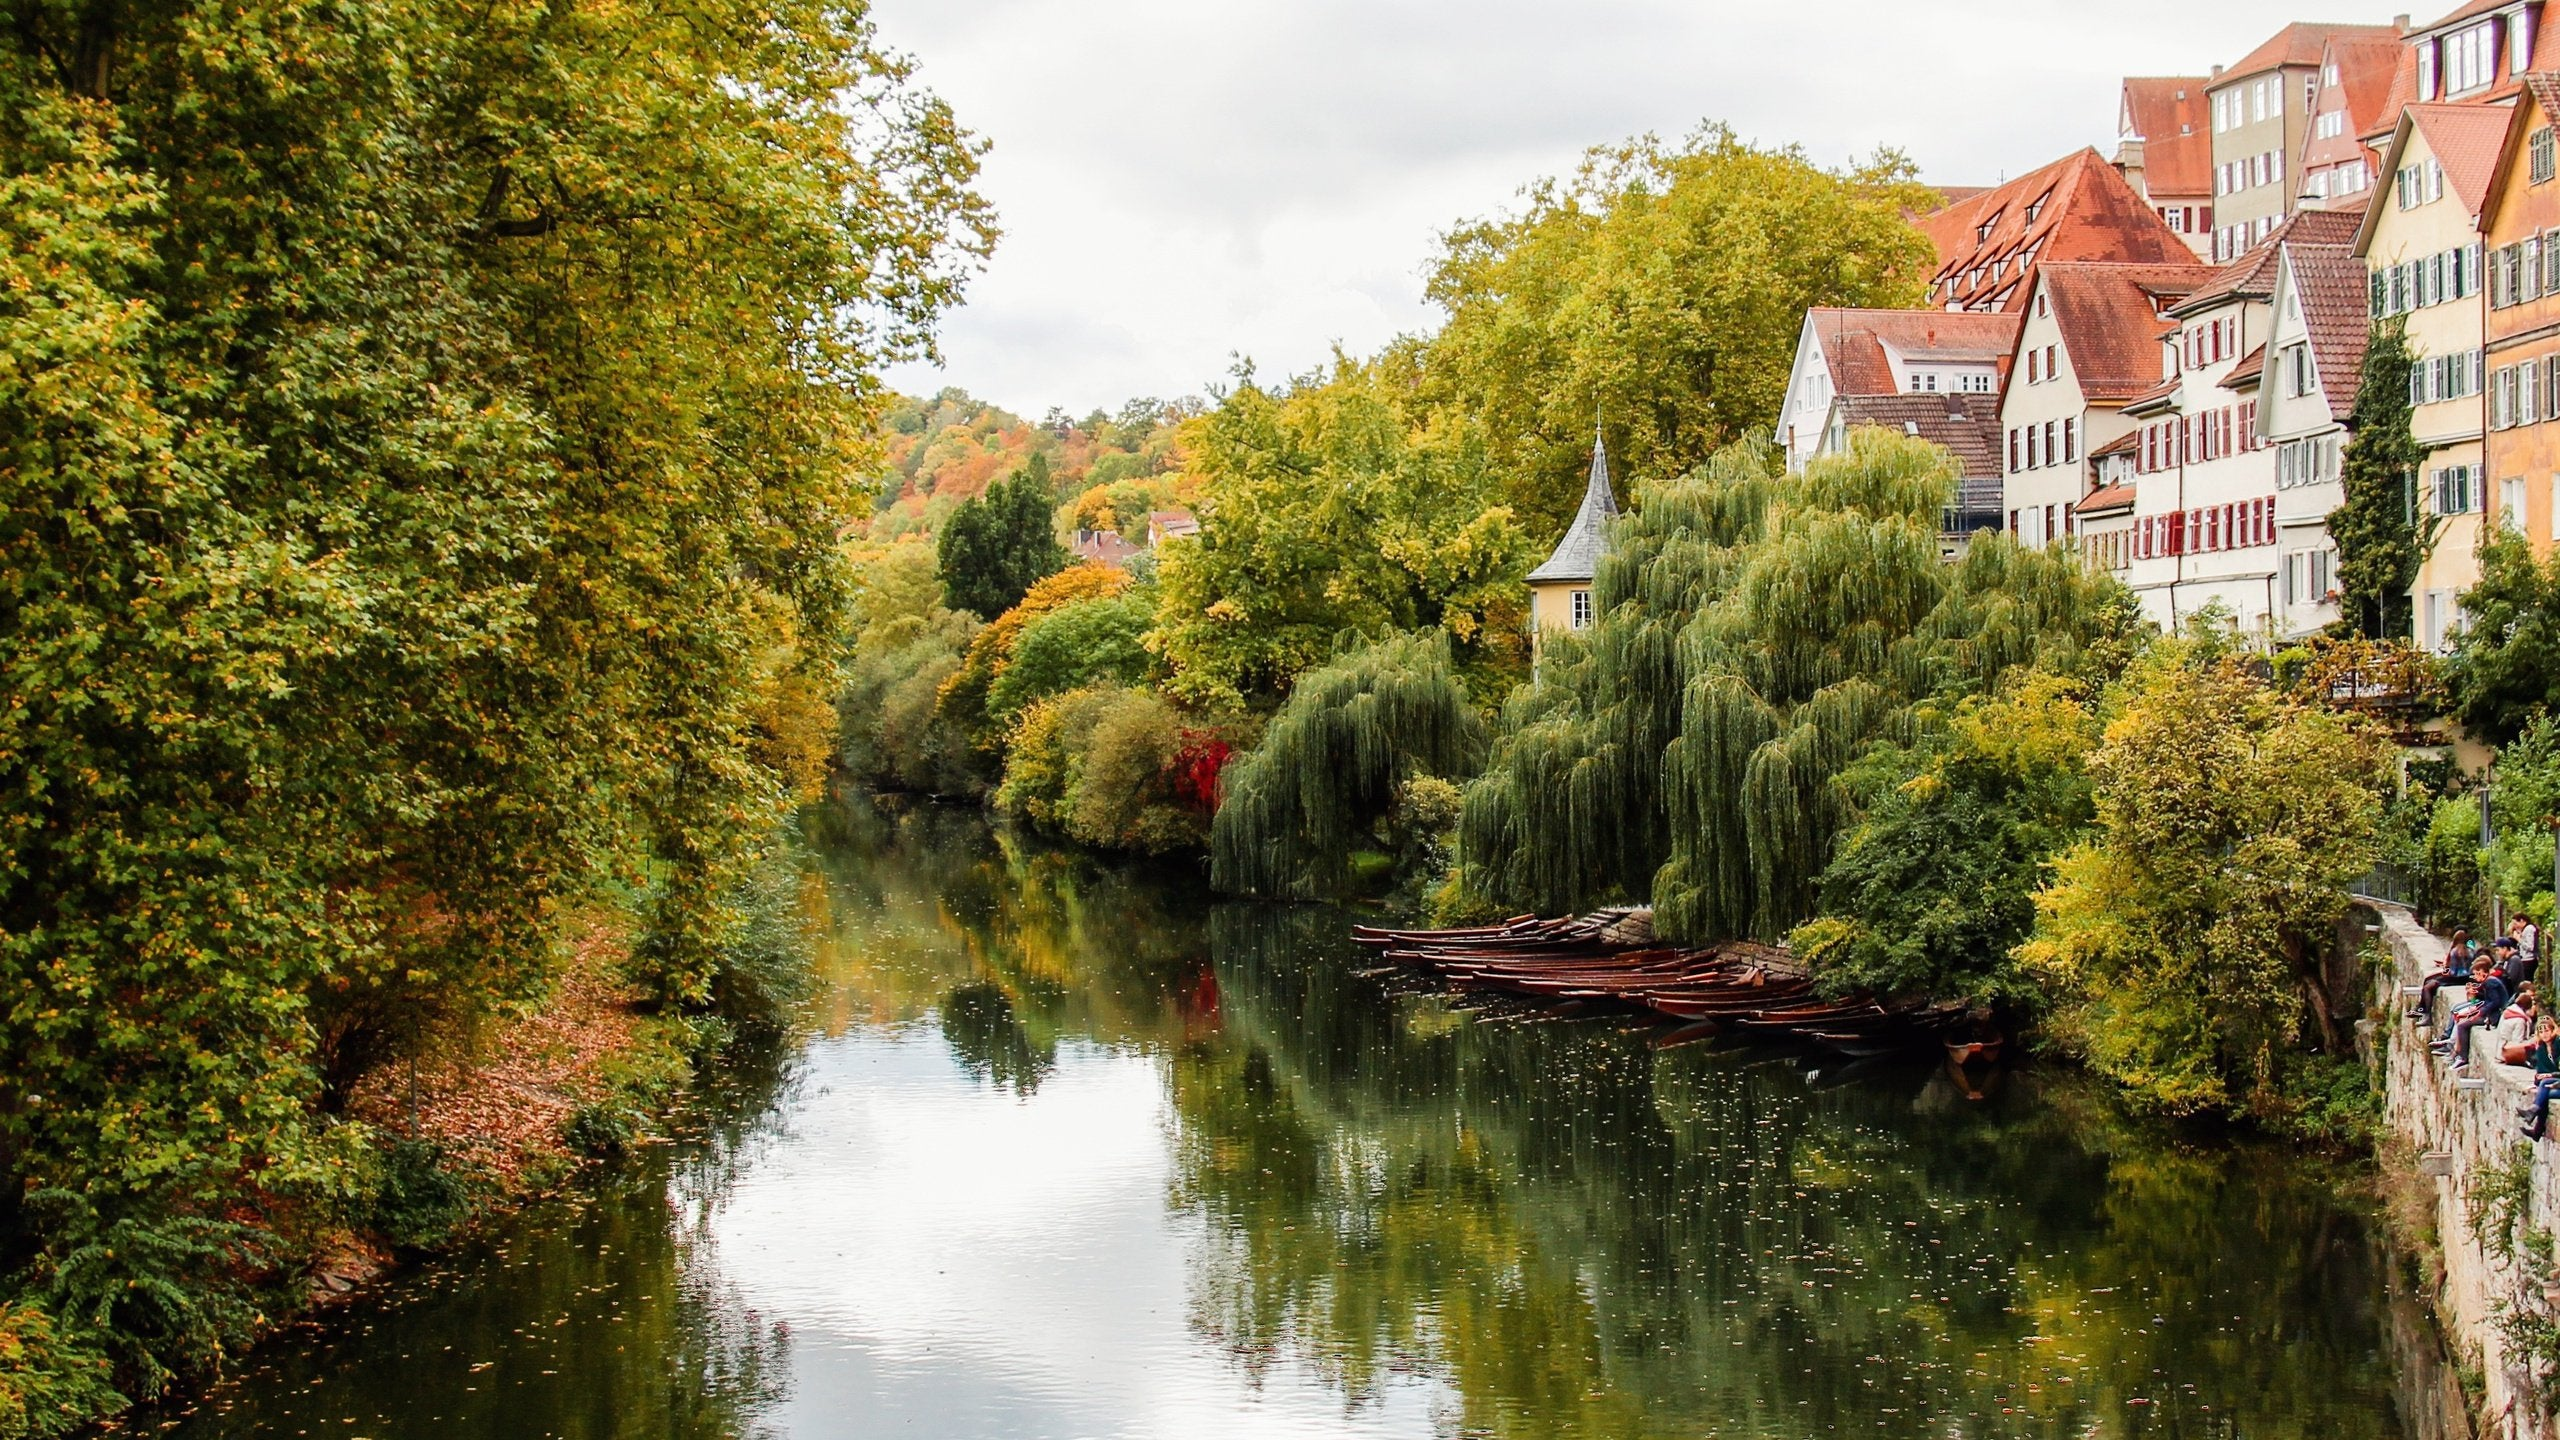
\includegraphics[width=\textwidth]{pictures/tubingenPicture.jpeg}
    % We see coarse structures at the first glance but finer details by staring at the picture for more time. 
    \label{fig:tubingen}
\end{figure}
\end{frame}

\begin{frame}{Visual Grouping}
    
\end{frame}

\begin{frame}{Visual Grouping}
\begin{figure}
    \centering
    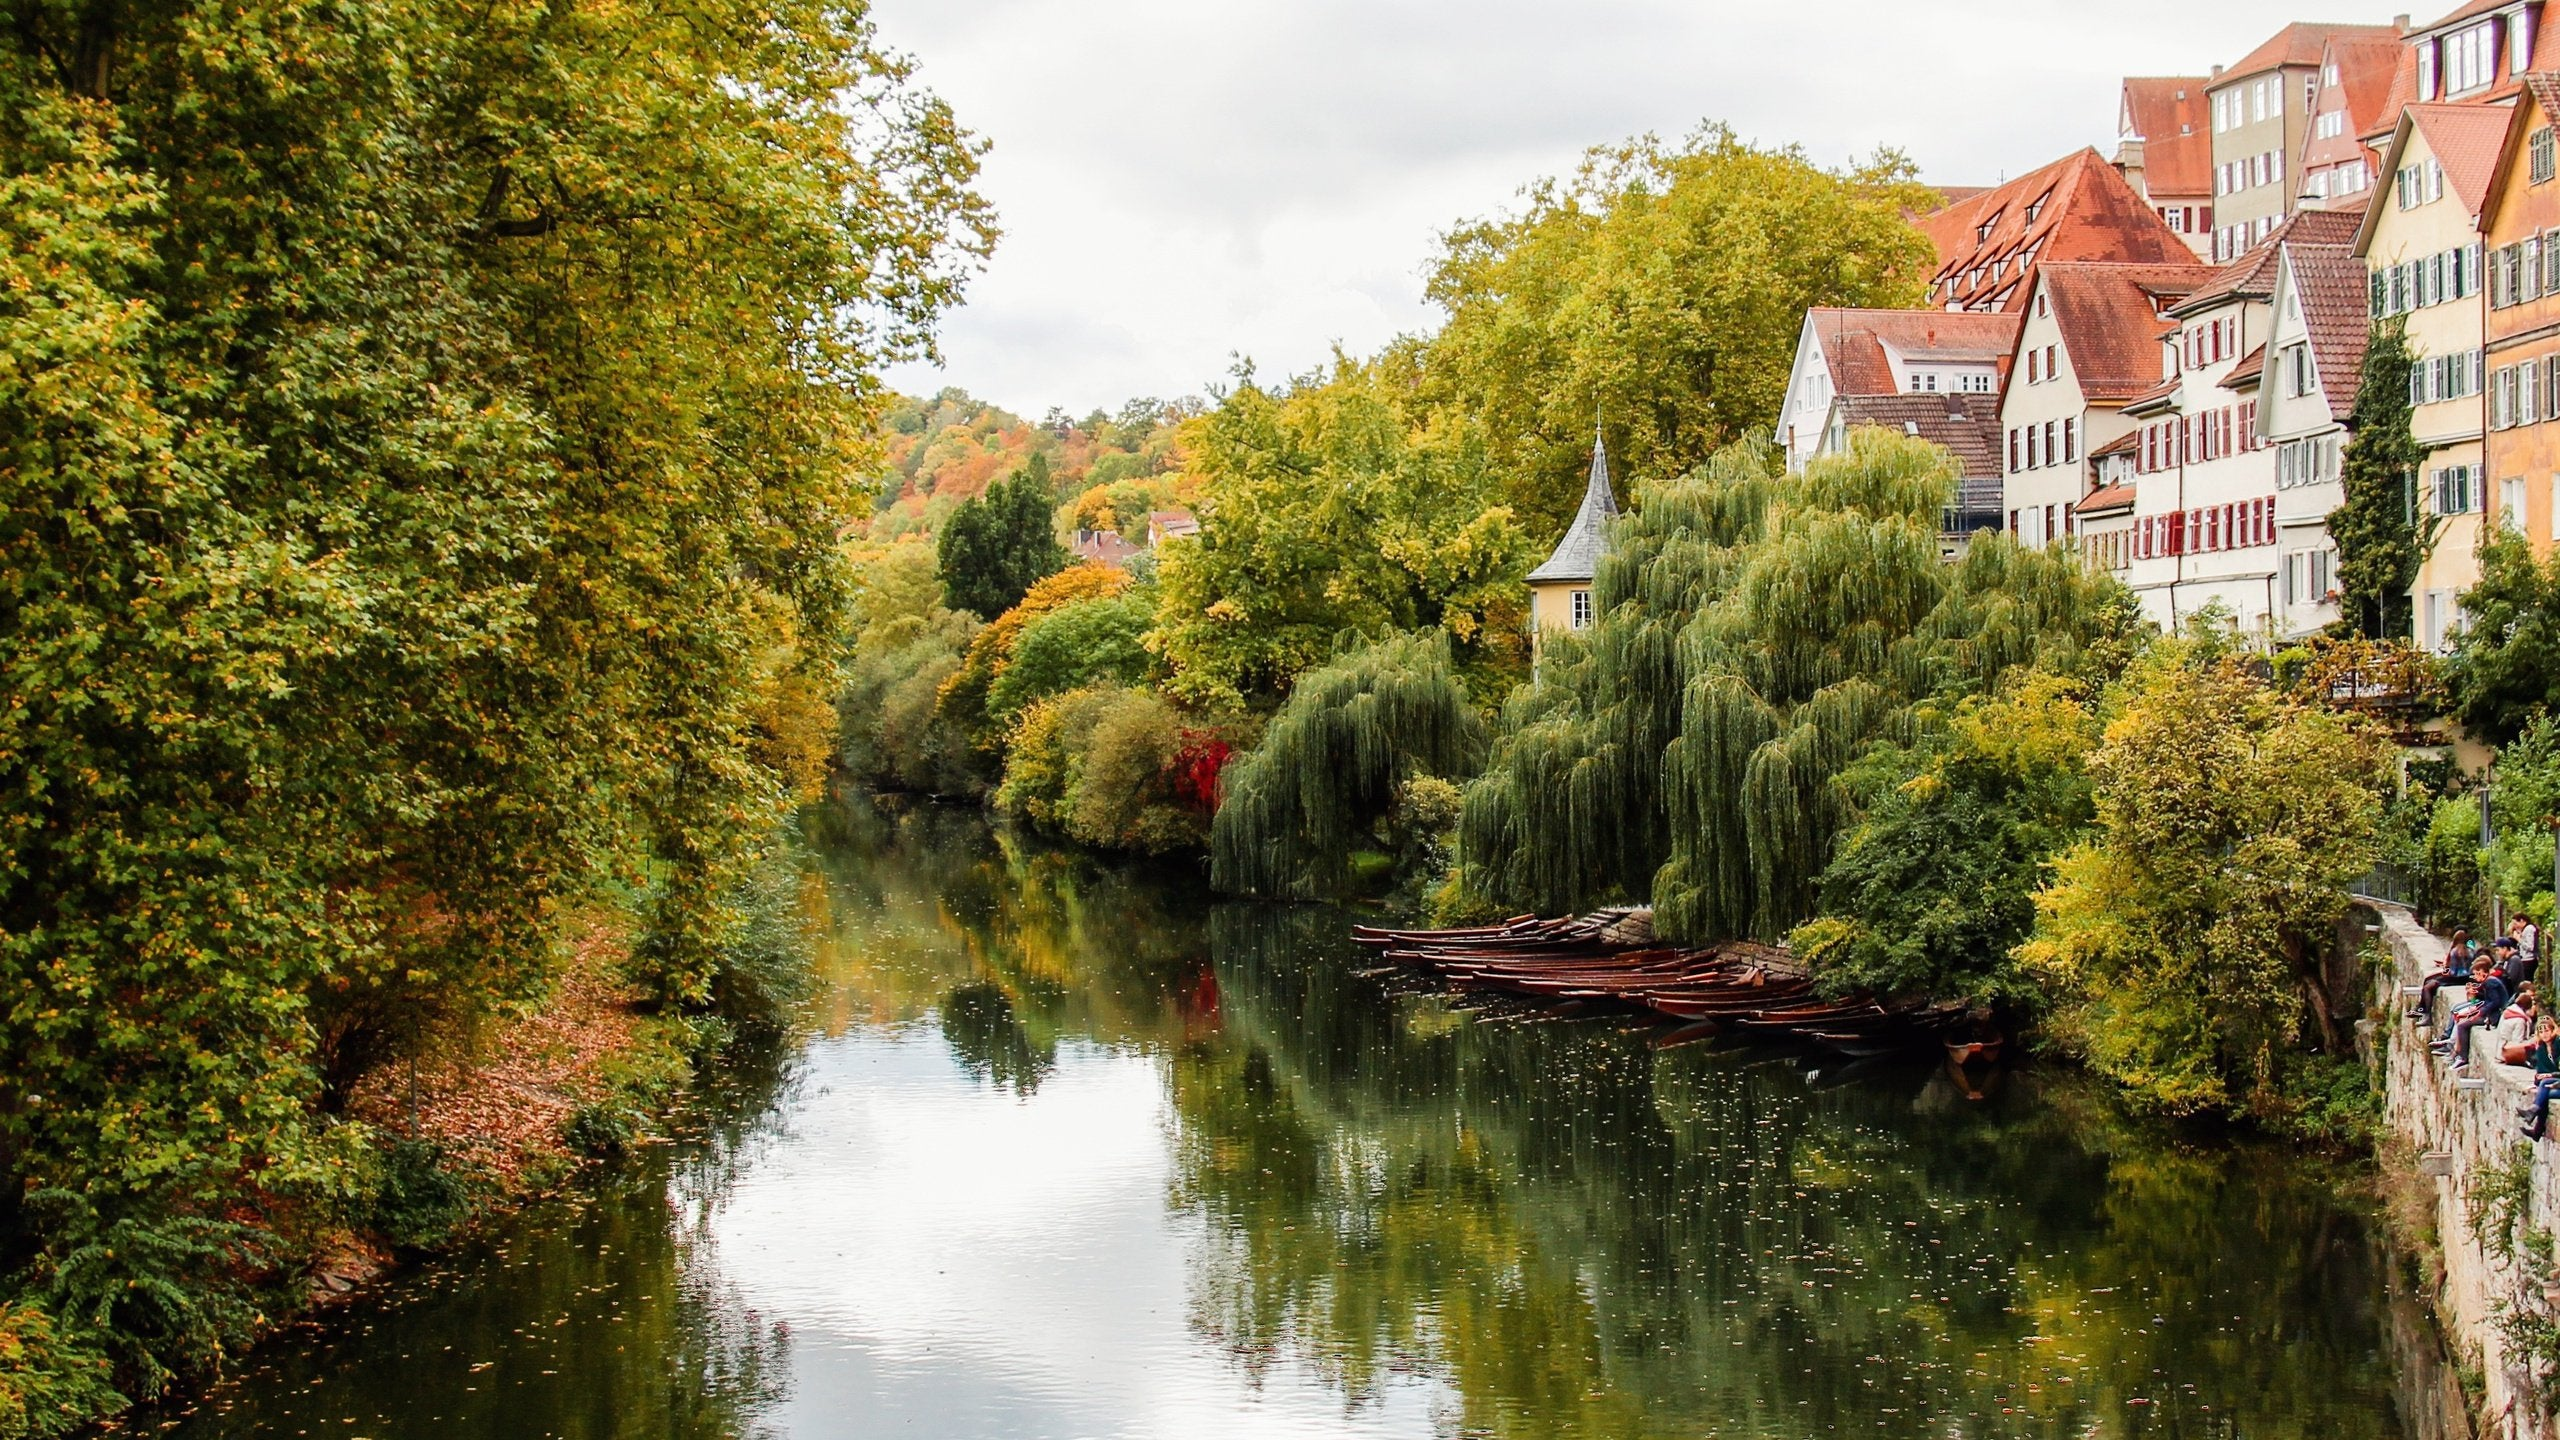
\includegraphics[width=\textwidth]{pictures/tubingenPicture.jpeg}
    % We see coarse structures at the first glance but finer details by staring at the picture for more time. 
    \label{fig:tubingen}
\end{figure}
\end{frame}

\begin{frame}{Perceptual Grouping Retains a Hierarchical Structure}
    \begin{figure}
        \centering
        \begin{subfigure}{0.3\textwidth}
            \centering
            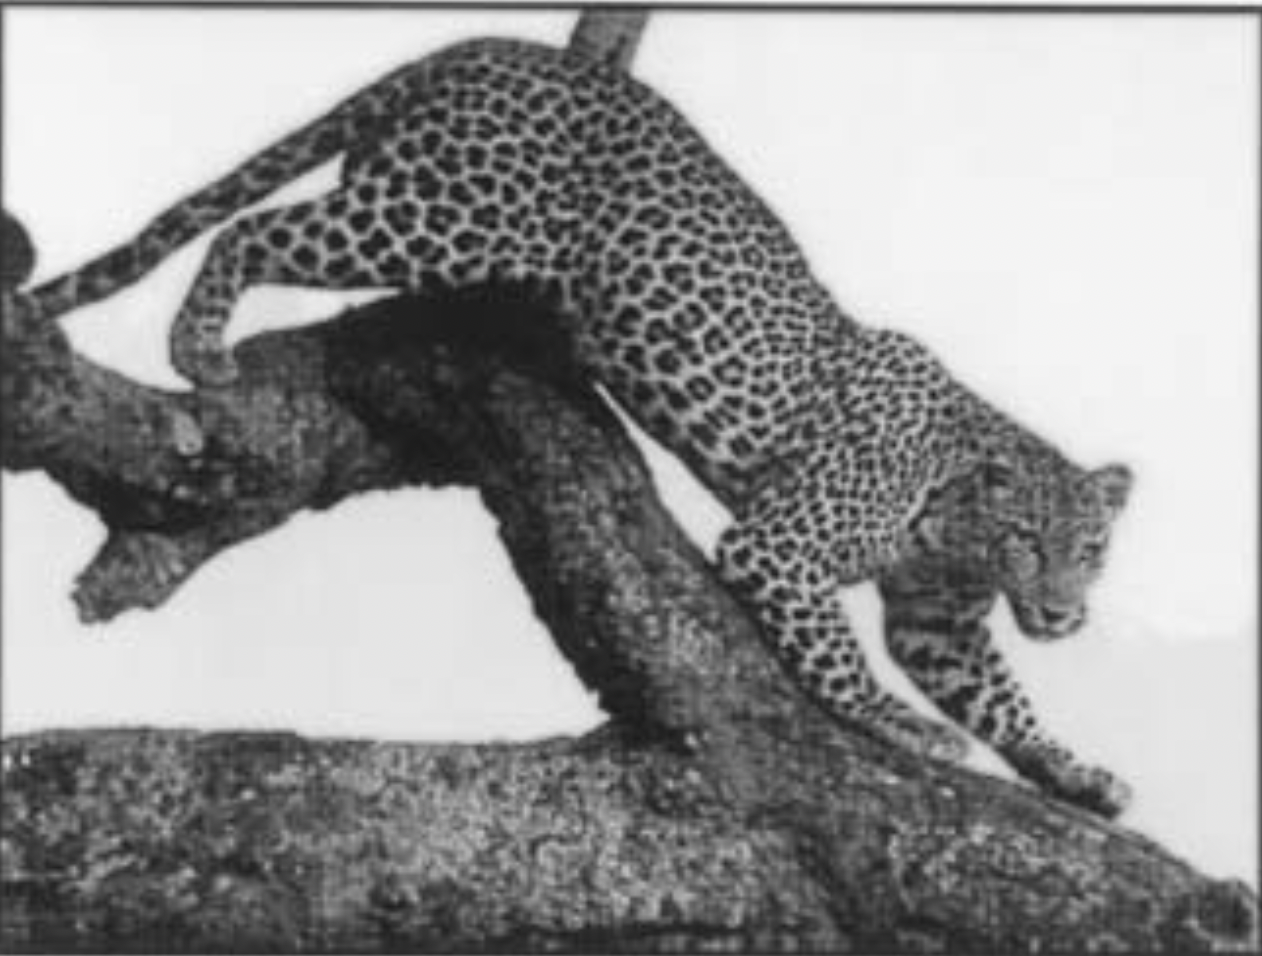
\includegraphics[width=\textwidth]{pictures/perceptualOrganization_1.png}
            \label{fig:perceptualOrg_a}
            \caption{}
        \end{subfigure}
        \hfill
        \begin{subfigure}{0.3\textwidth}
            \centering
            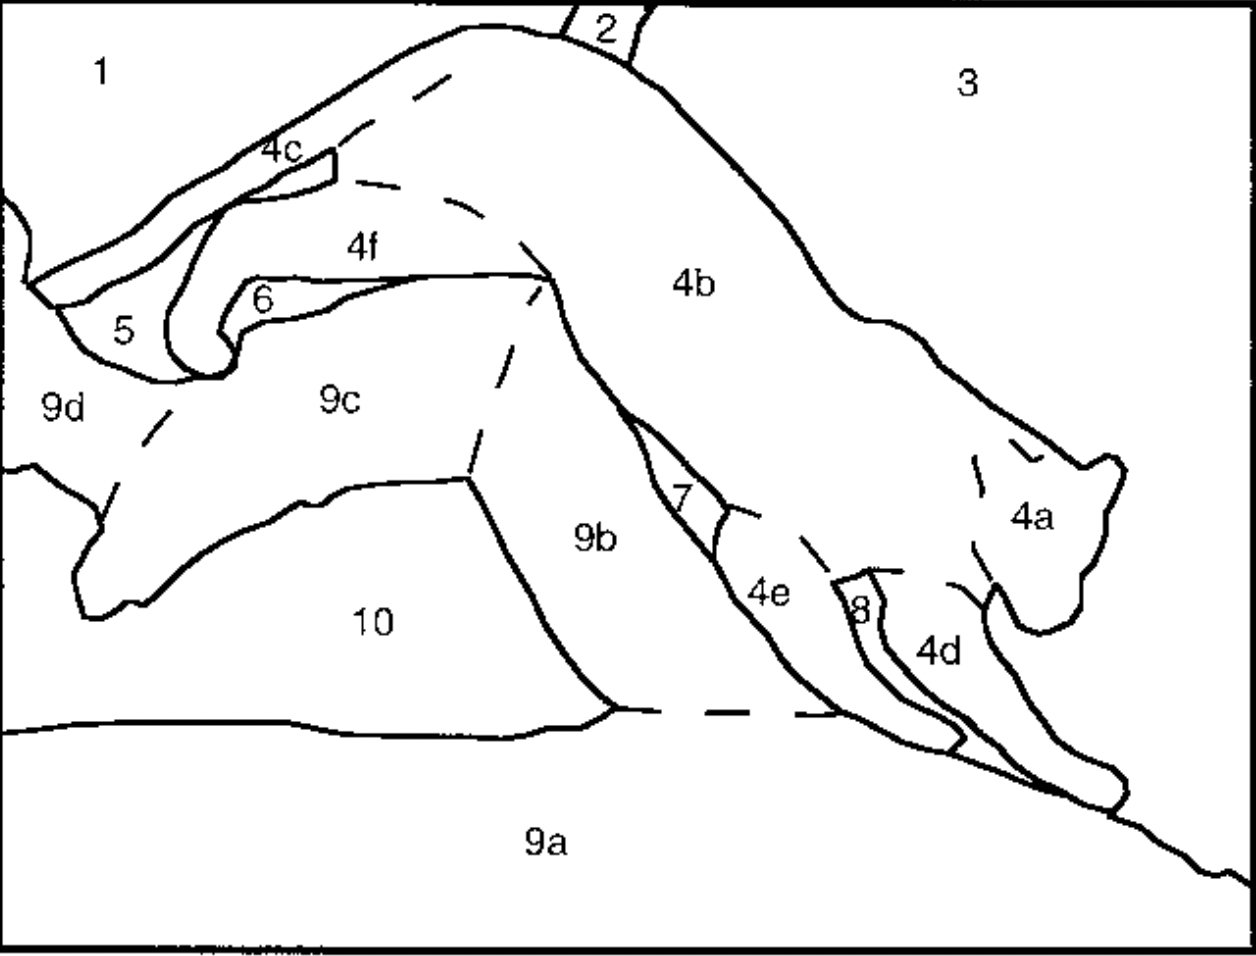
\includegraphics[width=\textwidth]{pictures/perceptualOrganization_2.png}
            \caption{}
            \label{figure:perceptualOrg_b}
        \end{subfigure}
        \hfill
        \begin{subfigure}{0.32\textwidth}
            \centering
            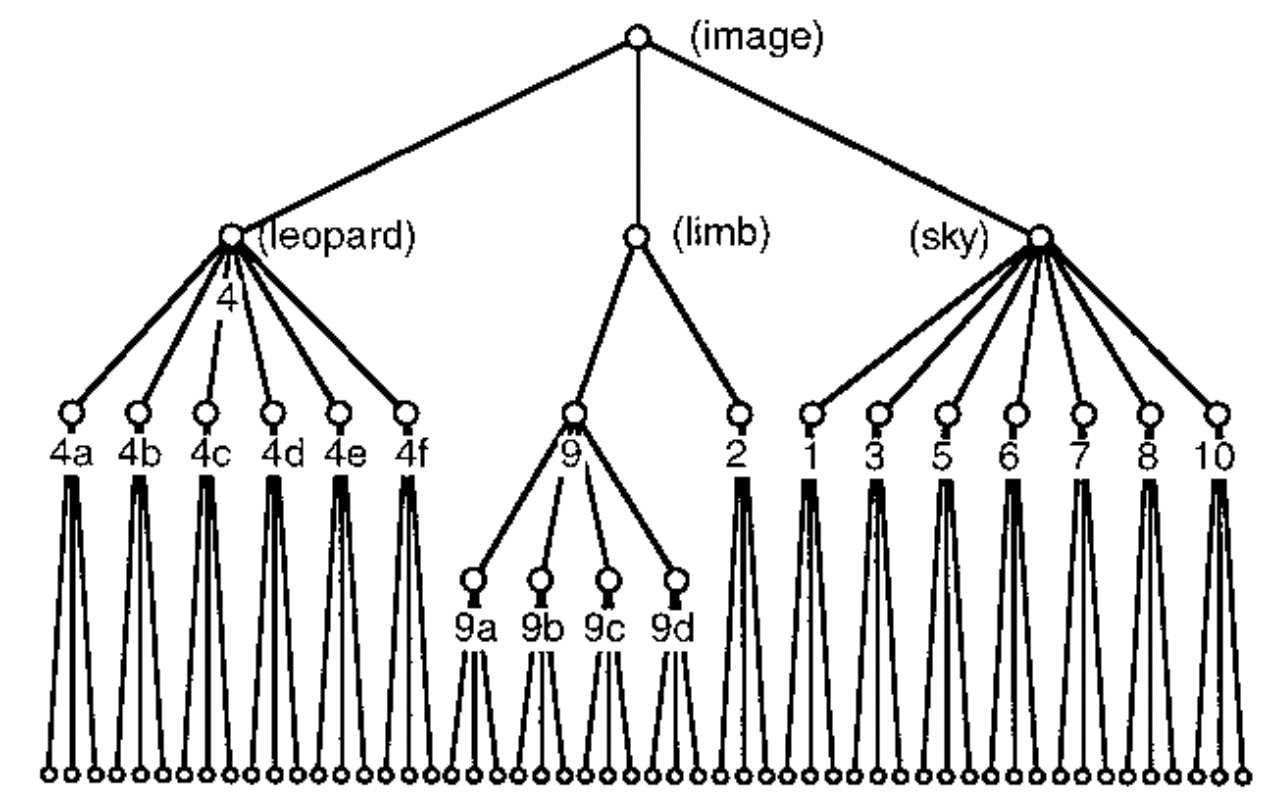
\includegraphics[width=\textwidth]{pictures/perceptualOrganization_3.png}
            \caption{}
            \label{figure:perceptualOrg_c}
        \end{subfigure}
    \caption{Perception of this image (1a) is organized into structured components (\ref{figure:perceptualOrg_b}). These structure components can be described by a hierarchical graph (\ref{figure:perceptualOrg_c}), with coarser components in the shallower layers, and finer components in deeper layers.
    
    \\
    {\footnotesize Adapted from \textcite{RN212}}
        }
    \label{fig:perceptual_org}
    \end{figure}
    
\end{frame}



\end{frame}

\begin{frame}{Hierarchical Perceptual Grouping and Exposure Time}
\begin{itemize}
    \item We decompose visual observation into hierarchical structures.
    \pause
    % \item How does hierarchical perceptual grouping behavior change with increasing exposure time?
    \item The fineness of the perceived hierarchical graph seems to relate to exposure time. 
    \pause
\end{itemize}
    
\metroset{block=fill}
\begin{exampleblock}{\textsc{Hypothesis}}
As more computational resources are allocated, perceptual grouping behavior gets refined and finer segments can be detected.
\end{exampleblock}

\begin{itemize}
    \item Can we relate this phenomenon to computation with a limited amount of resources?
\end{itemize}
\end{frame}


%%%%%%%%%%%%%%%%%%%%%%%%%%%%%%%%%%%%%%%%%%%%
\section{Segmentation}




\begin{frame}{Representing Images with Graph Networks}
    \begin{itemize}
        \item Represent each hexagon as a node.
        \item Connect each pair of hexagon by an edge.
    \end{itemize}

\begin{figure}
        \centering
        \resizebox{6 cm}{!}{%
        \begin{tikzpicture}[node distance={15mm}, thick,square/.style={regular polygon,regular polygon sides=4}] 
        
        \node(1) [fill=grey!10, square, draw] {$v_1$};
        \node[main] (2) [fill=grey!10, square, draw, below of=1] {$v_2$}; 
        \node[main] (3) [fill=grey!20, square, draw, below of=2] {$v_3$};
        \node[main] (4) [fill=grey!23, square, draw, right of=1] {$v_4$}; 
        \node[main] (5) [fill=grey!25, square, draw, below of=4] {$v_5$};
        \node[main] (6) [square, draw, below of=5] {$v_6$};
        \node[main] (7) [square, draw, right of=4] {$v_7$}; 
        \node[main] (8) [square, draw, below of=7] {$v_8$};
        \node[main] (9) [square, draw, below of=8] {$v_9$}; 
        
        \path (1) edge (2)
              (1) edge [bend right=45] (3)
              (1) edge (4)
              (1) edge [bend left=45] (7)
              
              (2) edge (3)
              (2) edge (5)
              (2) edge [bend left=45] (8)
              
              (3) edge (6)
              (3) edge [bend left=45] (9)
              (4) edge (5)
              (4) edge [bend right=45] (6)
              (4) edge (7)
              
              (5) edge (6)
              (5) edge (8)
              (6) edge (9)
              (7) edge (8)
              (7) edge [bend right=45] (9)
              (8) edge (9)
        \end{tikzpicture}
        }
    \caption{Example representation of 3x3 image with a graph network}
    \label{fig:my_label}
    \end{figure}

\end{frame}


\begin{frame}{Representing Images with Graph Networks}
    \begin{itemize}
        \item Assign computed weights to the edges.
    \end{itemize}

\begin{figure}
        \centering
        \resizebox{6 cm}{!}{%
        \begin{tikzpicture}[node distance={15mm}, thick,square/.style={regular polygon,regular polygon sides=4}] 
        
        \node(1) [fill=grey!10, square, draw] {$v_1$};
        \node[main] (2) [fill=grey!10, square, draw, below of=1] {$v_2$}; 
        \node[main] (3) [fill=grey!20, square, draw, below of=2] {$v_3$};
        \node[main] (4) [fill=grey!23, square, draw, right of=1] {$v_4$}; 
        \node[main] (5) [fill=grey!25, square, draw, below of=4] {$v_5$};
        \node[main] (6) [square, draw, below of=5] {$v_6$};
        \node[main] (7) [square, draw, right of=4] {$v_7$}; 
        \node[main] (8) [square, draw, below of=7] {$v_8$};
        \node[main] (9) [square, draw, below of=8] {$v_9$}; 
        
        \path 
              (3) edge (6)
              (4) edge [bend right=45] (6)
              (4) edge (7)
              (5) edge (6)
              (5) edge (8)

              (1) edge [bend left=45] (7)
              (2) edge [bend left=45] (8)
              (3) edge [bend left=45] (9);
        
        \path[line width = 1.2pt]
              (1) edge (4)
              (2) edge (5);
              
        \path[line width = 2pt] 
              (1) edge (2)
              (1) edge [bend right=45] (3)
              (2) edge (3)
              (6) edge (9)
              (7) edge (8)
              (7) edge [bend right=45] (9)
              (8) edge (9)
              (4) edge (5);
              
        \end{tikzpicture}
        }
    \caption{Representation of 3x3 image with a weighted graph network}
    \label{fig:image_graph_weighted}
    \end{figure}

\end{frame}

\begin{frame}{Segmentation with Norm Min Cut}
    \begin{figure}[ht!]
    \hspace*{-1cm} 
    \centering
        \begin{subfigure}{0.3\textwidth}
        \vspace{-0.5cm}
        \centering
        \begin{tikzpicture}[node distance={12mm},  scale=1, thick, every square/.style={regular polygon,regular polygon sides=4}, transform shape]
        
        \node(1) [fill=grey!10, square, draw] {$v_1$};
        \node[main] (2) [fill=grey!10, square, draw, below of=1] {$v_2$}; 
        \node[main] (3) [fill=grey!14, square, draw, below of=2] {$v_3$};
        \node[main] (4) [fill=grey!23, square, draw, right of=1] {$v_4$}; 
        \node[main] (5) [fill=grey!25, square, draw, below of=4] {$v_5$};
        \node[main] (6) [square, draw, below of=5] {$v_6$};
        \node[main] (7) [square, draw, right of=4] {$v_7$}; 
        \node[main] (8) [square, draw, below of=7] {$v_8$};
        \node[main] (9) [square, draw, below of=8] {$v_9$}; 
        
        \path (3) edge (6)
              (4) edge [bend right=45] (6)
              (4) edge (7)
              (5) edge (6)
              (5) edge (8)

              (1) edge [bend left=45] (7)
              (2) edge [bend left=45] (8)
              (3) edge [bend left=45] (9);
        
        \path[line width = 1.2pt]
              (1) edge (4)
              (2) edge (5)
              (2) edge (3);
              
        \path[line width = 2pt] 
              (1) edge (2)
              (1) edge [bend right=45] (3)
              (2) edge (3)
              (6) edge (9)
              (7) edge (8)
              (7) edge [bend right=45] (9)
              (8) edge (9)
              (4) edge (5);
              
            
        \end{tikzpicture}
        \caption{Graph before cut}
        \end{subfigure}
        \hfill
        \begin{subfigure}{0.3\textwidth}
        \centering
            \begin{tikzpicture}[node distance={12mm},  scale=1, thick, every square/.style={regular polygon,regular polygon sides=4}, transform shape]
                \node(1) [fill=grey!10, square, draw] {$v_1$};
                \node[main] (2) [fill=grey!10, square, draw, below of=1] {$v_2$}; 
                \node[main] (3) [fill=grey!14, square, draw, below of=2] {$v_3$};
                \node[main] (4) [fill=grey!23, square, draw, right of=1] {$v_4$}; 
                \node[main] (5) [fill=grey!25, square, draw, below of=4] {$v_5$};
                \node[main] (6) [square, draw, below of=5] {$v_6$};
                \node[main] (7) [square, draw, right of=4] {$v_7$}; 
                \node[main] (8) [square, draw, below of=7] {$v_8$};
                \node[main] (9) [square, draw, below of=8] {$v_9$}; 
                
            \path[line width = 2pt] 
                  (1) edge (2)
                  (1) edge [bend right=45] (3)
                  (2) edge (3)
                  (4) edge (5)
                  (7) edge (8)
                  (8) edge (9)
                  (6) edge (9);

            \path[line width = 1.2pt] 
                  (1) edge (4)
                  (2) edge (5);
                  
                                   
 
            \end{tikzpicture}
            \caption{Graph after the first cut}
        \end{subfigure}
        \hfill
        \begin{subfigure}{0.32\textwidth}
        \centering
            \begin{tikzpicture}[node distance={12mm},  scale=1, thick, every square/.style={regular polygon,regular polygon sides=4}, transform shape] 
        
                \node(1) [fill=grey!10, square, draw] {$v_1$};
                \node[main] (2) [fill=grey!10, square, draw, below of=1] {$v_2$}; 
                \node[main] (3) [fill=grey!14, square, draw, below of=2] {$v_3$};
                \node[main] (4) [fill=grey!23, square, draw, right of=1] {$v_4$}; 
                \node[main] (5) [fill=grey!25, square, draw, below of=4] {$v_5$};
                \node[main] (6) [square, draw, below of=5] {$v_6$};
                \node[main] (7) [square, draw, right of=4] {$v_7$}; 
                \node[main] (8) [square, draw, below of=7] {$v_8$};
                \node[main] (9) [square, draw, below of=8] {$v_9$}; 
                
                \path[line width = 2pt] (1) edge (2)
                      (2) edge (3)
                      (4) edge (5)
                      
                      (7) edge (8)
                      (8) edge (9)
                      (6) edge (9)
              
            \end{tikzpicture}
        \caption{Graph after the second cut}
        \end{subfigure}
    \caption{An example segmentation of a graph}
    \end{figure}
    
        
\end{frame}

\begin{frame}{Generating Images with No Inductive Biases}
    \begin{columns}
    \column{0.4\textwidth}
    \begin{figure}
        \centering
        
\includegraphics[width=\textwidth]{pictures/grid_init2.png}        
    \end{figure}
    \vspace{-0.62cm}
    \begin{figure}
        \centering
        
\includegraphics[width=\textwidth]{pictures/grid_init3.png}
    \end{figure}
    
    \column{0.6\textwidth}
    \underline{\textsc{Criteria:}}
    \begin{itemize}
        \item We need images that induce no bias
        \item There should be no semantic meaning assigned to the images
        \item There should be no effect of object recognition
    \end{itemize}  

    \end{columns}
\end{frame}

\begin{frame}{Segmentation with Norm Min Cut}
\begin{enumerate}
    \item Apply Normalized Min Cut algorithm to find the ground truth segments.
\end{enumerate}
\end{frame}

\begin{frame}{Segmentation - \textit{Normalized Min Cut}}
\begin{figure}
    \hspace*{-1em}
    \vspace*{-1em}
    \begin{tikzpicture}
      [
        grow                    = right,
        sibling distance        = 14em,
        level distance          = 17em,
        edge from parent/.style = {draw, -latex},
        every node/.style       = {font=\footnotesize},
        scale = 0.46,
        sloped
      ]
      \node(0) {
\includegraphics[width=0.2\textwidth]{pictures/grid_init4.png}}
            child {node (seg1) {
\includegraphics[width=0.2\textwidth]{pictures/seg_2_cut1.png}}
                }
            child {node (seg2) {
\includegraphics[width=0.2\textwidth]{pictures/seg_3_cut1.png}}
                child {node (segLastBottom) {
\includegraphics[width=0.2\textwidth]{pictures/seg_4_cut2.png}}}
                child {node (segLastTop) {
\includegraphics[width=0.2\textwidth]{pictures/seg_5_cut2.png}}
                    child {node (seg7) {
\includegraphics[width=0.2\textwidth]{pictures/seg_7_cut3.png}}}
                    child {node (seg6) {
\includegraphics[width=0.2\textwidth]{pictures/seg_6_cut3.png}}}
                }
                };
        \node (Cut1) [above of=seg2, yshift=0.7cm] {Cut 1};
        \node (Cut2) [above of=segLastTop, yshift=0.5cm] {Cut 2};
        \node (Cut3) [above of=seg6, yshift=0.5cm] {Cut 3};
    \end{tikzpicture}
    \caption{First three steps of segmentation}
    \label{fig:gridSegmentationExample}
    
\end{figure}
\end{frame}


\begin{frame}{Finding Segments}
\begin{enumerate}
    \item Apply Normalized Min Cut algorithm to find the ground truth segments.
    \item Assign cut orders depending on the \textit{Ncut} value.
\end{enumerate}
\end{frame}


\begin{frame}{Finding Segments}
\begin{figure}
    \centering
    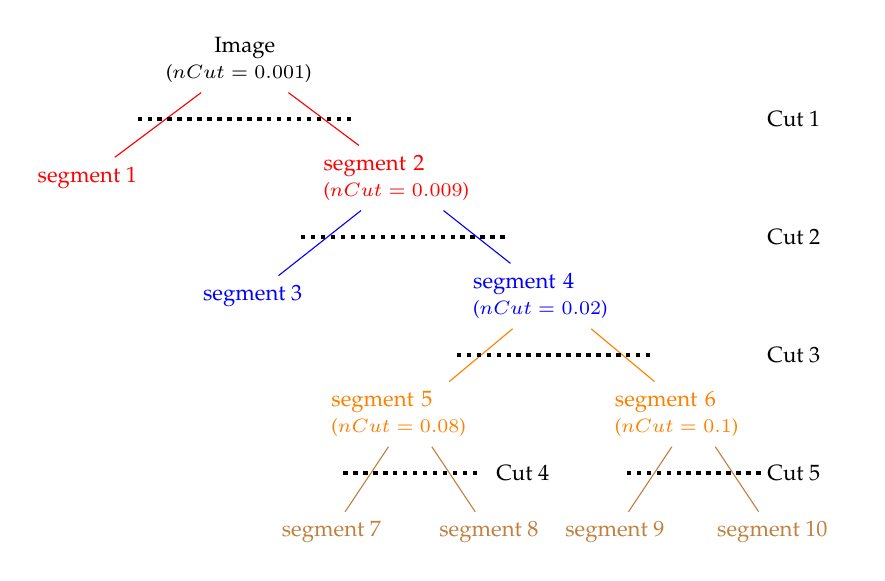
\begin{tikzpicture}
        [
            level 1/.style = {red, sibling distance = 4cm},
            level 2/.style = {blue, sibling distance = 3.8cm},
            level 3/.style = {orange, sibling distance = 3.6cm},
            level 4/.style = {brown, sibling distance = 2cm},
            every node/.style       = {font=\footnotesize}
        ]
        \node(0) [text width=2cm]{\centering Image\\\centering \smaller($nCut=0.001$)}
            child {node {segment 1}
            }
            child {node [text width=2cm]{segment 2\\\smaller($nCut=0.009$)}
            child {node {segment 3}}
            child {node [text width=2cm] {segment 4\\\smaller ($nCut=0.02$)}
                child {node [text width=2cm] {segment 5\\\smaller($nCut=0.08$)}
                    child {node {segment 7}}
                    child {node {segment 8}}}
                child {node [text width=2cm] {segment 6\\\smaller($nCut=0.1$)}
                    child {node {segment 9}}
                    child {node {segment 10}}
                    }
                }
                };
                
        \draw[dotted, ultra thick, transform canvas={xshift=-1em}] ($ (0)!.5!(0-2)$) ++ (+20pt, 0) -- ($ (0)!.5!(0-1) $) ++ (-50pt,0) node[right, xshift=9.6cm] (cut1) {Cut 1}; 
        \draw[dotted, ultra thick,transform canvas={xshift=-1em}] ($ (0-2)!.5!(0-2-2)$) ++ (20pt,0) -- ($ (0-2)!.5!(0-2-1) $) node[right, below of=cut1, yshift=-0.5cm] (cut2) {Cut 2}; 
        \draw[dotted, ultra thick,transform canvas={xshift=-1em}] ($ (0-2-2)!.5!(0-2-2-2)$) ++ (20pt,0) -- ($ (0-2-2)!.5!(0-2-2-1) $) node[right, below of=cut2, yshift=-0.5cm] (cut3) {Cut 3};
        \draw[dotted, ultra thick,transform canvas={xshift=-1em}] ($ (0-2-2-1)!.5!(0-2-2-1-2)$) ++ (20pt,0) -- ($ (0-2-2-1)!.5!(0-2-2-1-1) $) node[right, xshift=+1.8cm] (cut4) {Cut 4};
        \draw[dotted, ultra thick,transform canvas={xshift=-1em}] ($ (0-2-2-2)!.5!(0-2-2-2-2)$) ++ (20pt,0) -- ($ (0-2-2-2)!.5!(0-2-2-2-1) $) node[right, below of=cut3, yshift=-0.5cm] (cut5) {Cut 5};
    \end{tikzpicture}
    \caption{Found segments}
\end{figure}
\end{frame}

\begin{frame}{Finding Segments}
\begin{enumerate}
    \item Apply Normalized Min Cut algorithm to find the ground truth segments.
    \item Assign cut orders depending on the \textit{Ncut} value.
    \item Stop when all the segments are found.
    \item Use only the leaf nodes.
\end{enumerate}
\end{frame}

\begin{frame}{Finding Segments}
\begin{figure}
    \centering
    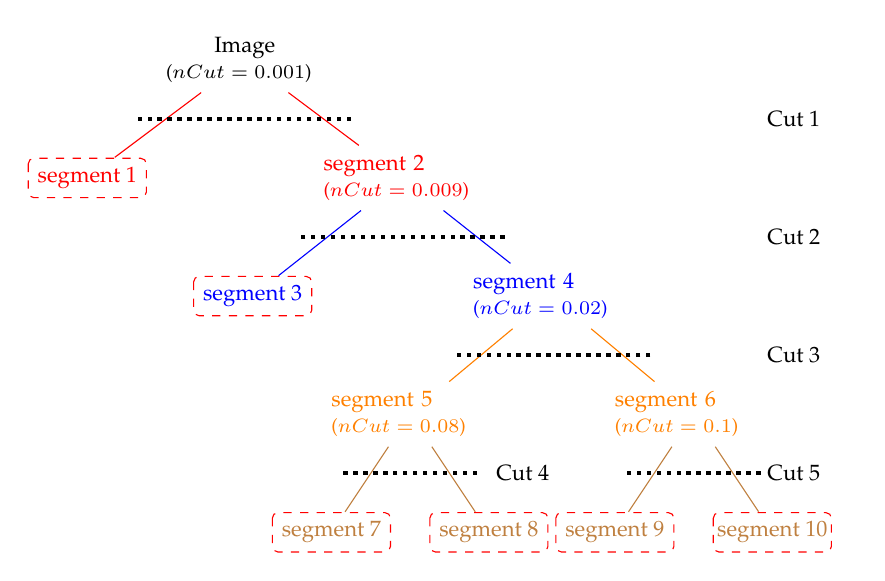
\begin{tikzpicture}
        [
            level 1/.style = {red, sibling distance = 4cm},
            level 2/.style = {blue, sibling distance = 3.8cm},
            level 3/.style = {orange, sibling distance = 3.6cm},
            level 4/.style = {brown, sibling distance = 2cm},
            every node/.style       = {font=\footnotesize}
        ]
        \node(0) [text width=2cm]{\centering Image\\\centering \smaller($nCut=0.001$)}
            child {node {segment 1}
            }
            child {node [text width=2cm]{segment 2\\\smaller($nCut=0.009$)}
            child {node {segment 3}}
            child {node [text width=2cm] {segment 4\\\smaller ($nCut=0.02$)}
                child {node [text width=2cm] {segment 5\\\smaller($nCut=0.08$)}
                    child {node {segment 7}}
                    child {node {segment 8}}}
                child {node [text width=2cm] {segment 6\\\smaller($nCut=0.1$)}
                    child {node {segment 9}}
                    child {node {segment 10}}
                    }
                }
                };
        \draw[dashed,rounded corners=2, red]($(0-1)+(-.75,+.25)$)rectangle($(0-1)+(.75,-.25)$); % Draw rectangles from northwest to southeast
        \draw[dashed,rounded corners=2, red]($(0-2-1)+(-.75,+.25)$)rectangle($(0-2-1)+(.75,-.25)$);     
        \draw[dashed,rounded corners=2, red]($(0-2-2-2-2)+(-.75,+.25)$)rectangle($(0-2-2-2-2)+(.75,-.25)$); 
        \draw[dashed,rounded corners=2, red]($(0-2-2-2-1)+(-.75,+.25)$)rectangle($(0-2-2-2-1)+(.75,-.25)$); 
        \draw[dashed,rounded corners=2, red]($(0-2-2-1-1)+(-.75,+.25)$)rectangle($(0-2-2-1-1)+(.75,-.25)$); 
        \draw[dashed,rounded corners=2, red]($(0-2-2-1-2)+(-.75,+.25)$)rectangle($(0-2-2-1-2)+(.75,-.25)$); 
        \draw[dotted, ultra thick, transform canvas={xshift=-1em}] ($ (0)!.5!(0-2)$) ++ (+20pt, 0) -- ($ (0)!.5!(0-1) $) ++ (-50pt,0) node[right, xshift=9.6cm] (cut1) {Cut 1}; 
        \draw[dotted, ultra thick,transform canvas={xshift=-1em}] ($ (0-2)!.5!(0-2-2)$) ++ (20pt,0) -- ($ (0-2)!.5!(0-2-1) $) node[right, below of=cut1, yshift=-0.5cm] (cut2) {Cut 2}; 
        \draw[dotted, ultra thick,transform canvas={xshift=-1em}] ($ (0-2-2)!.5!(0-2-2-2)$) ++ (20pt,0) -- ($ (0-2-2)!.5!(0-2-2-1) $) node[right, below of=cut2, yshift=-0.5cm] (cut3) {Cut 3};
        \draw[dotted, ultra thick,transform canvas={xshift=-1em}] ($ (0-2-2-1)!.5!(0-2-2-1-2)$) ++ (20pt,0) -- ($ (0-2-2-1)!.5!(0-2-2-1-1) $) node[right, xshift=+1.8cm] (cut4) {Cut 4};
        \draw[dotted, ultra thick,transform canvas={xshift=-1em}] ($ (0-2-2-2)!.5!(0-2-2-2-2)$) ++ (20pt,0) -- ($ (0-2-2-2)!.5!(0-2-2-2-1) $) node[right, below of=cut3, yshift=-0.5cm] (cut5) {Cut 5};
    \end{tikzpicture}
    \caption{Found segments}
\end{figure}
\end{frame}

\begin{frame}{Finding Segments}
\begin{enumerate}
    \item Apply Normalized Min Cut algorithm to find the ground truth segments.
    \item Assign cut orders depending on the \textit{Ncut} value.
    \item Stop when all the segments are found.
    \item Use only the leaf nodes.
    \item Present segments depending on the cut order (5 cuts).
    \item Display segment with the average intensity of the initial image.
\end{enumerate}
\end{frame}

\begin{frame}[standout]{Display the Image - \textit{Cut Order 4}}
    \begin{figure}
        \centering
        \begin{subfigure}{0.4\textwidth}
        \centering
            
\includegraphics[width=0.8\textwidth]{pictures/grid_init4.png}
        \end{subfigure}
        \hfill
        \begin{subfigure}{0.4\textwidth}
            \centering
            
\includegraphics[width=0.8\textwidth]{pictures/seg_9_cut4.png}
        \end{subfigure}
    \end{figure}
\end{frame}

\begin{frame}{Testing the Algorithm}
    \begin{itemize}
        \metroset{block=fill}
        \begin{exampleblock}{\textsc{Research Question}}
            Can we relate hierarchical perceptual grouping phenomenon to computation with a limited amount of resources?
        \end{exampleblock}
        \pause
        \item We found a normalized cut algorithm that relates computation to deeper levels of hierarchical segmentation.
        \pause
        \item Does the order of segments discovery in a computational algorithm relate to human perceptual grouping, when perceiving the same images?
    \end{itemize}
\end{frame}



%%%%%%%%%%%%%%%%%%%%%%%%%%%%%%%%%%%%%%%%%%%%%%%
\section{Experimental Paradigms}
\begin{frame}{}
    \metroset{block=fill}
    \begin{exampleblock}{\textsc{Research Question}}
        Is the fineness of the perceived hierarchical graph related to exposure time?
    \end{exampleblock}
    \pause
    \begin{itemize}
        \item Experiment 1: Contrast sensitivity estimation
        \pause
        \item Experiment 2: Measure the effect of exposure time on segmentation
    \end{itemize}
\end{frame}


\begin{frame}{Experiment 1 - \textit{Contrast Sensitivity Estimation}}
    \begin{figure}
    \centering
        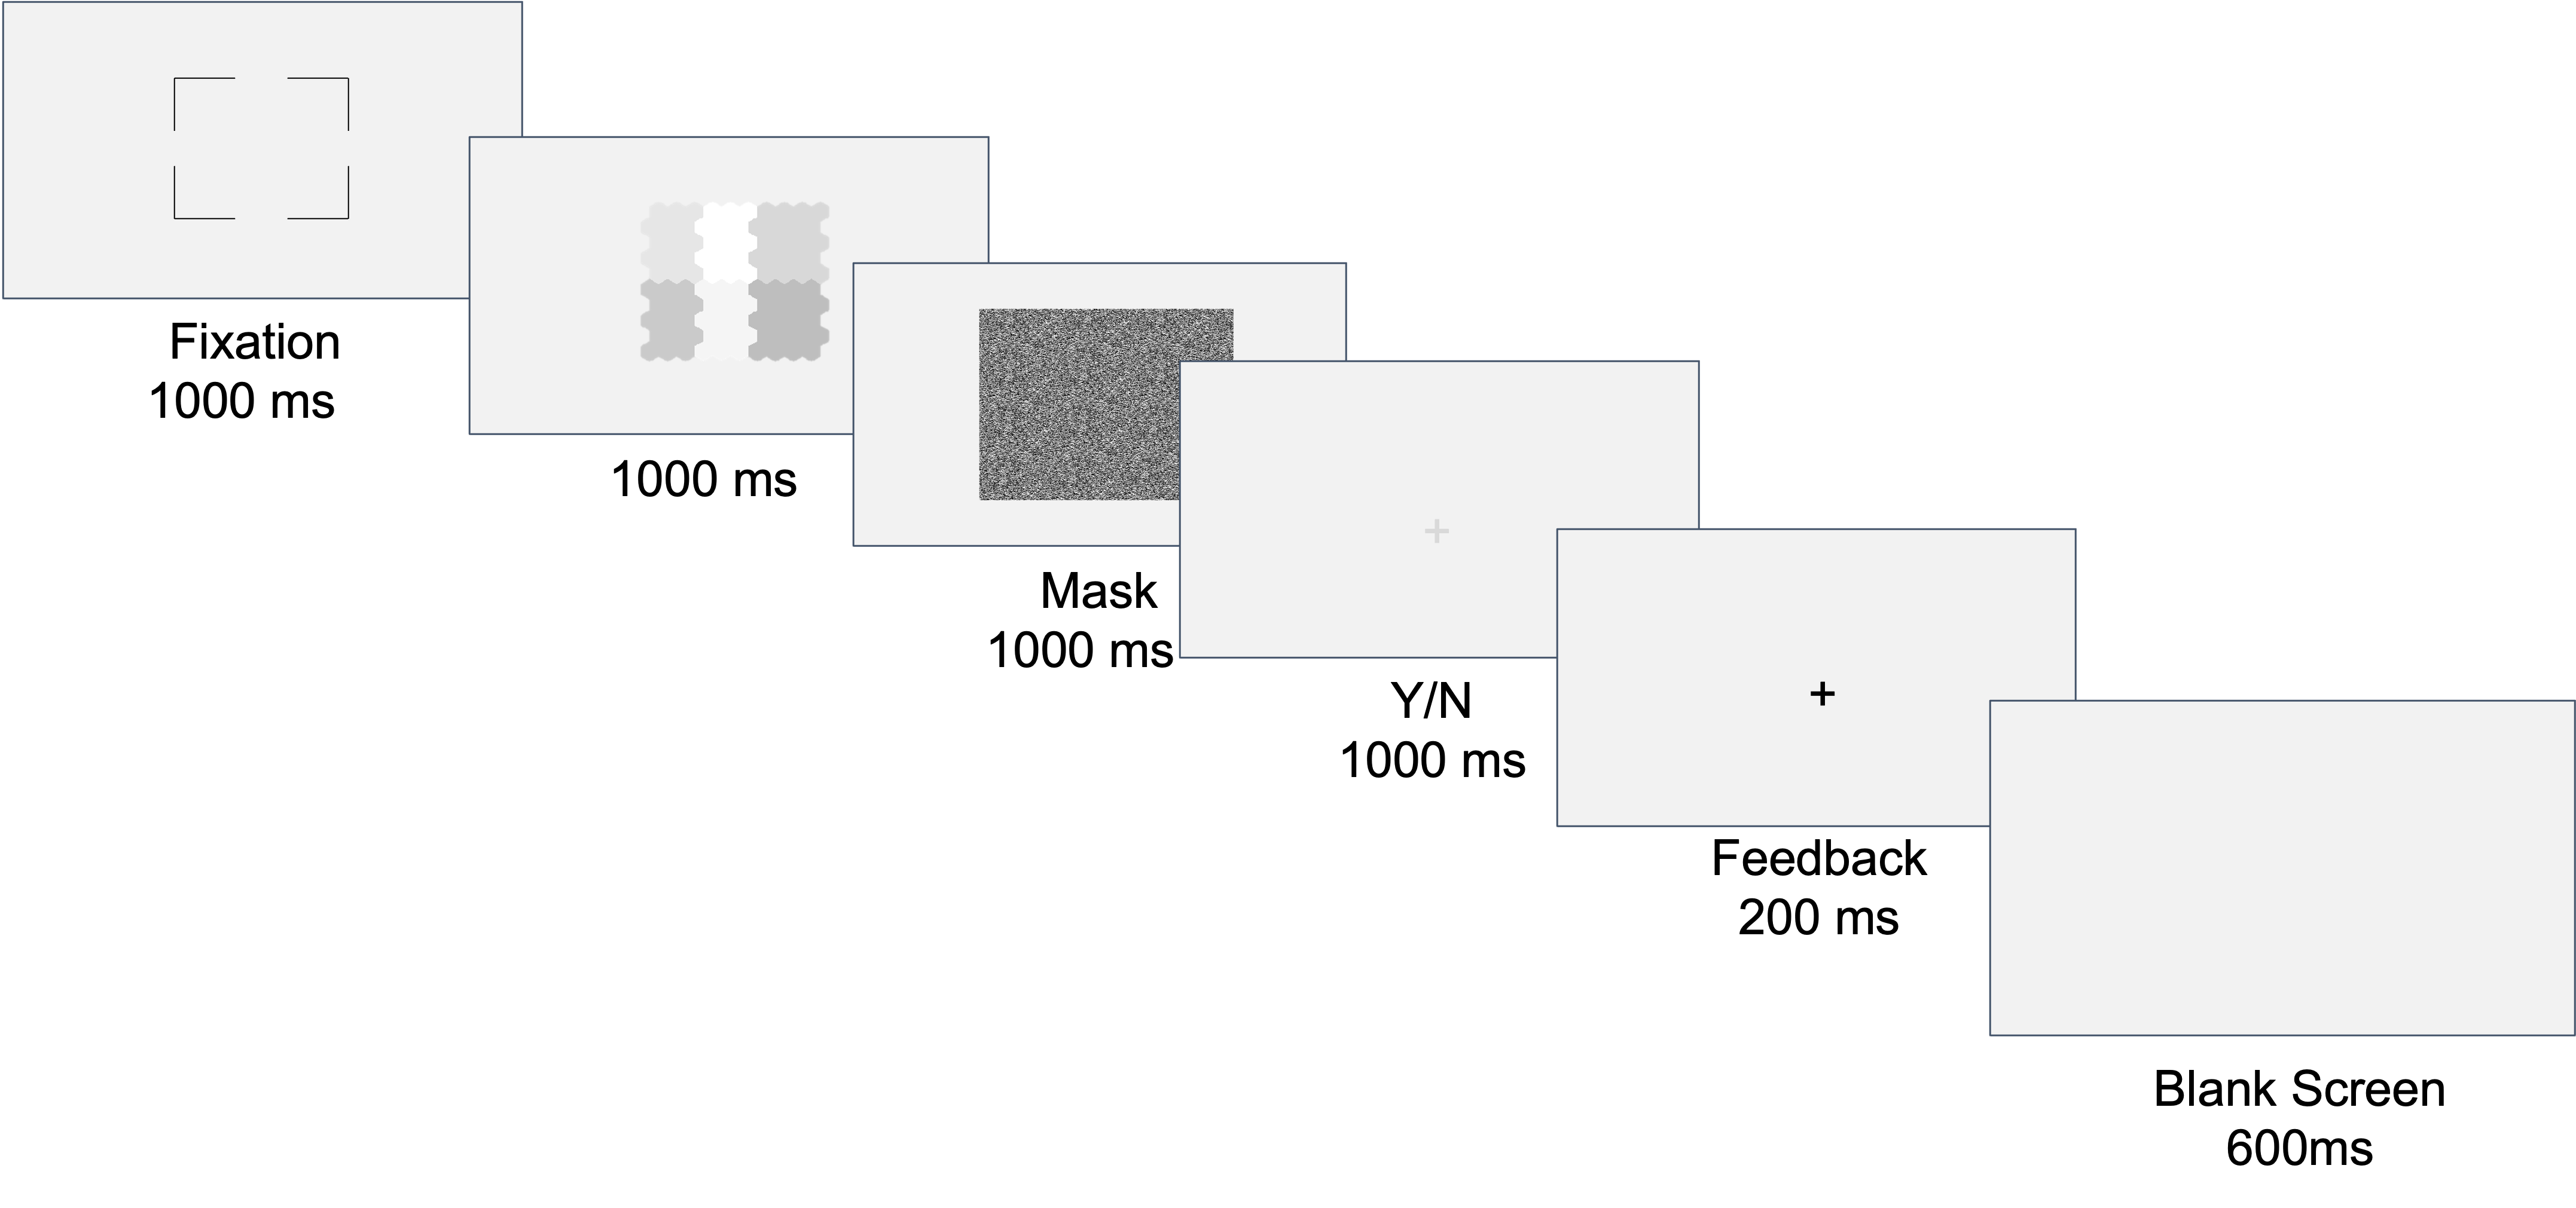
\includegraphics[width = \textwidth]{pictures/thresholdExpProcedure.png}   
    \caption{\footnotesize Estimating Individual Contrast Sensitivity}
    \end{figure}    
    \vspace{-0.5cm}
    \begin{itemize}
        \item Present 10x10 grid pattern with six different intensities
        \item Segment borders remain same
        \item Staircase Method (QUEST) to get contrast difference between segments ($\delta I$)
        \item "Did you detect 6 segments?"
    \end{itemize}
\end{frame}

\begin{frame}{Contrast Sensitivity Task - \textit{Psychometric Function}}
    \begin{figure}
        \centering
        \begin{figure}
        \centering
            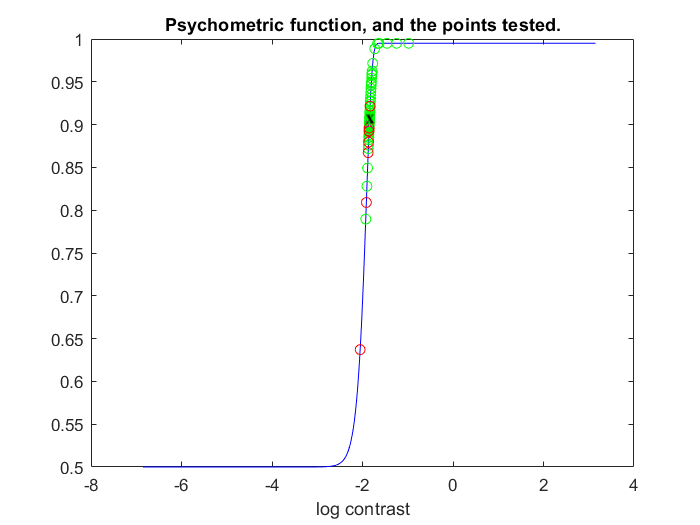
\includegraphics[width=0.6\textwidth]{pictures/thrExp_PC.png}
        \end{figure}
        \hfill
        \label{fig:psychometric_func}
        \vspace{-0.7cm}
        \caption{Psychometric function with 'Yes' and 'No' responses}
    \end{figure}
    \vspace{-0.5cm}
    \begin{itemize}
    \small
        \item Number of Trials:	  100
        \item Threshold Criterion: 0.9
        \item Beta:		  3.5 (Slope of the curve)
        \item Delta\Lapse:	 .01 (Probability of making mistakes above threshold)
        \item Gamma:		 .5 (Yes/No Task)        
        \item Create graded intensity levels with fixed intervals    
    \end{itemize}
\end{frame}

\begin{frame}{Experiment 2 - \textit{Main Task}}
\begin{figure}
\centering
    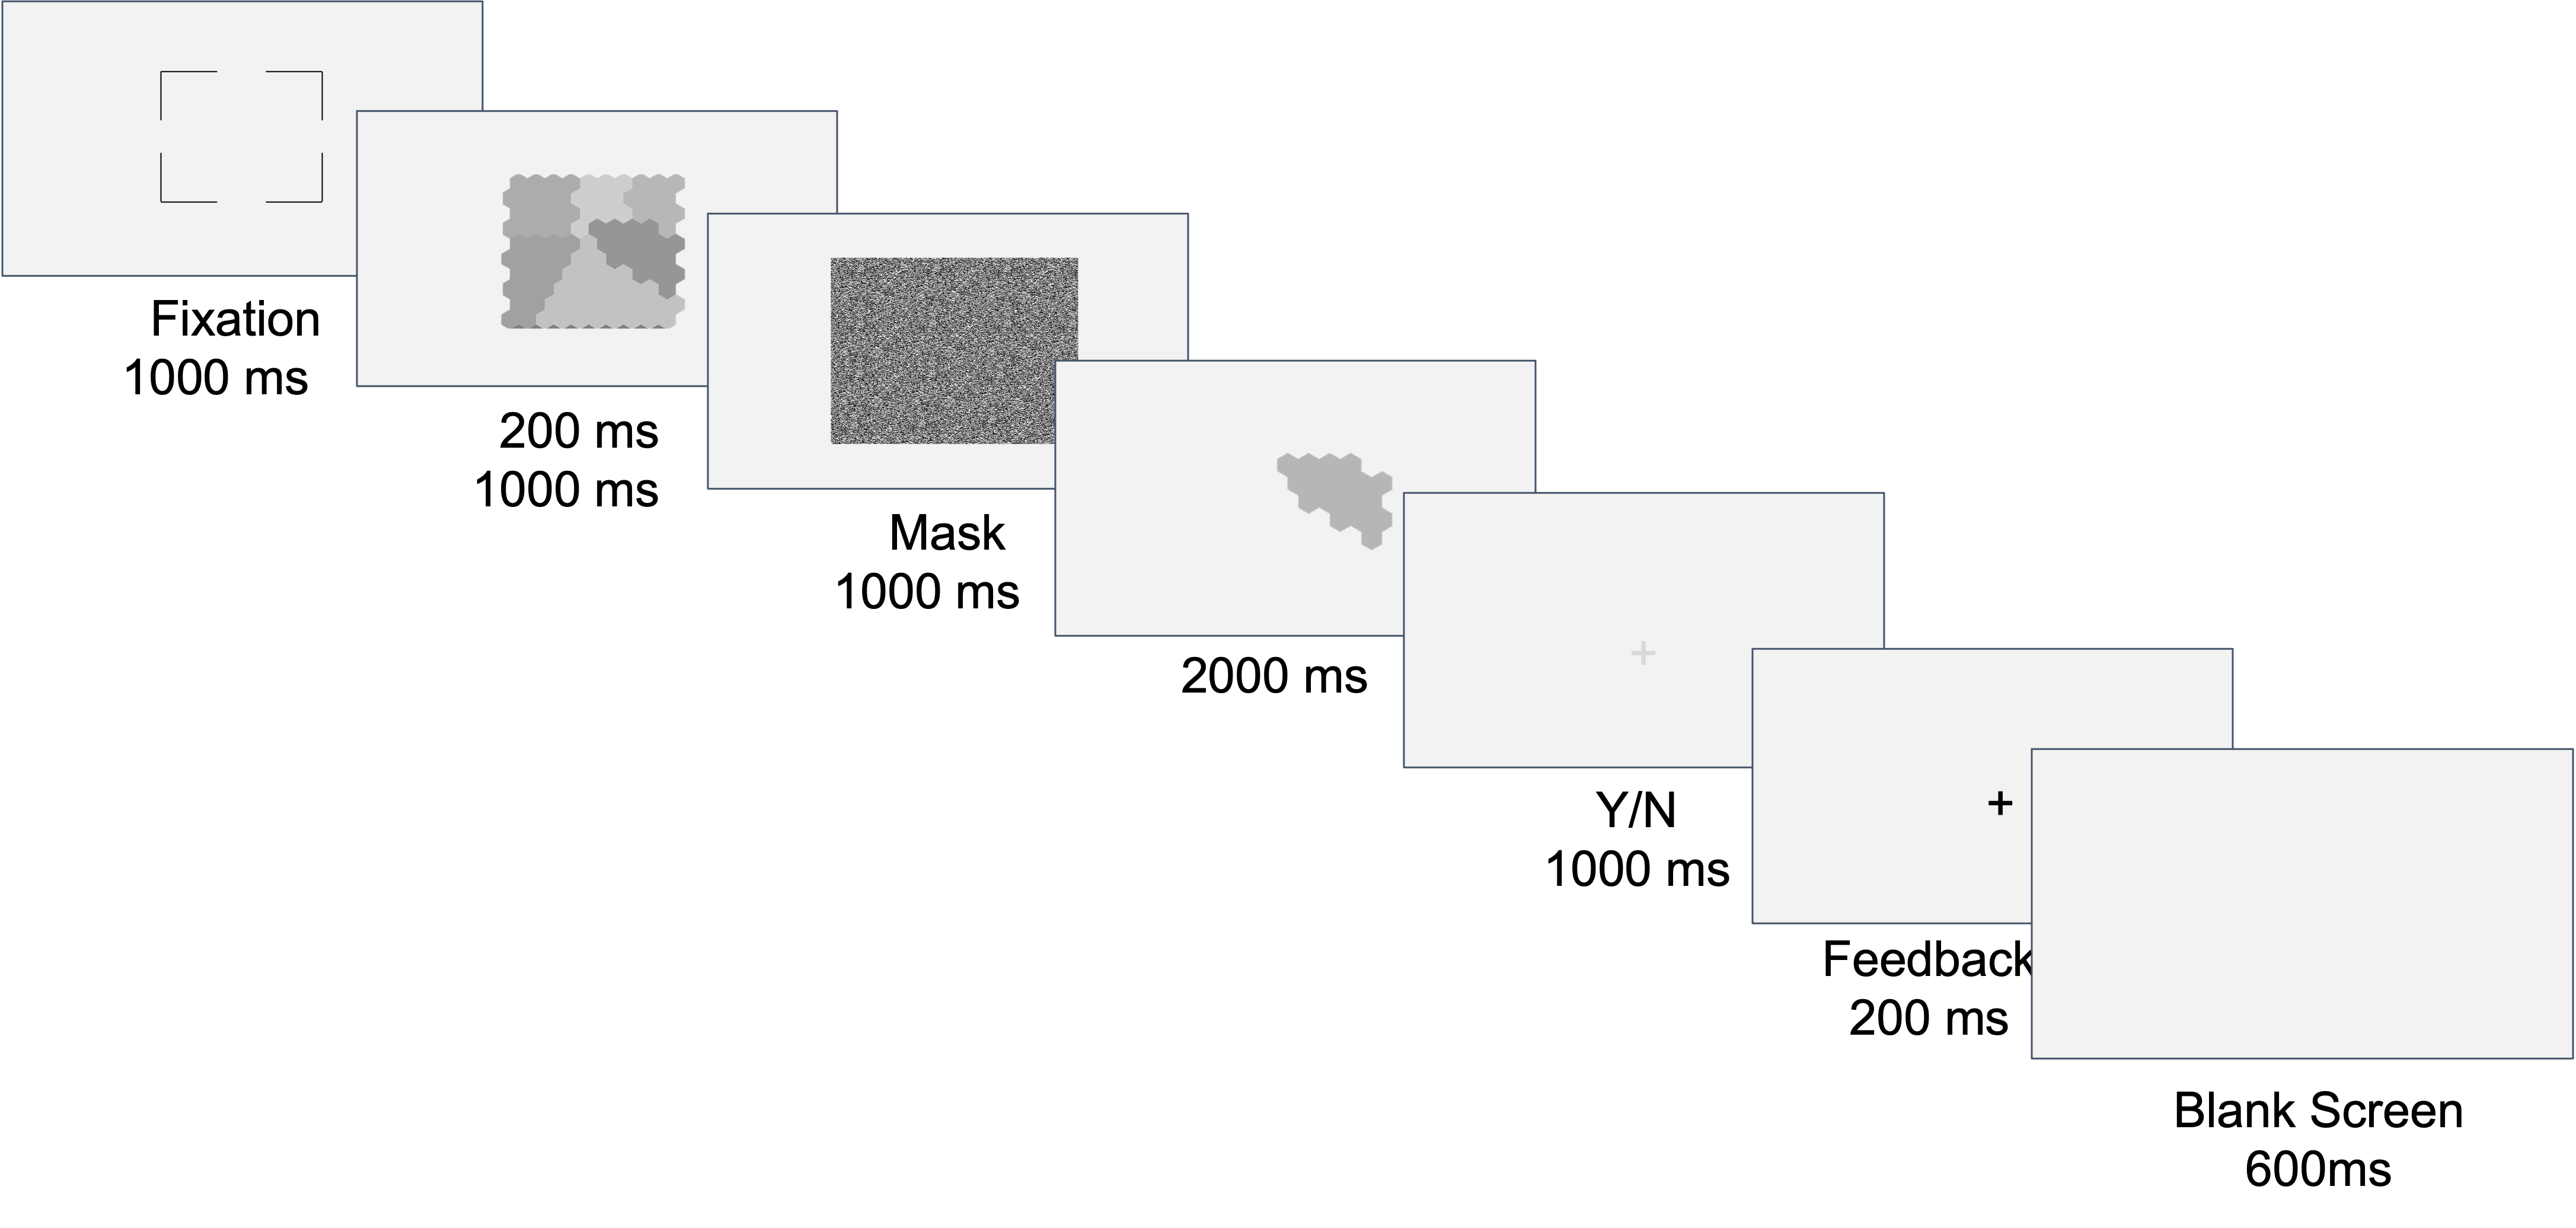
\includegraphics[width = \textwidth]{pictures/ExperimentalProcedure.png}   
\caption{\footnotesize Experimental Procedure}
\end{figure}

\begin{itemize}
    \footnotesize
    \item Present 10x10 grid pattern with six different intensities assigned randomly to each of groups 
    \item Present segments in average intensity value of the image
    \item Ask "Did you see the presented segment in the previously shown image?" (Y/N)
\end{itemize}
\end{frame}

\begin{frame}[standout]
\begin{figure}
    \begin{tikzpicture}
        %% Upper left
        \draw[thick] (-5,-5) -- (-4,-5);
        \draw[thick] (-5,-5) -- (-5,-6);
        %% Upper Right
        \draw[thick] (-2,-5) -- (-1,-5);
        \draw[thick] (-1,-5) -- (-1,-6);
        %% Bottom Left
        \draw[thick] (-5,-9) -- (-4,-9);
        \draw[thick] (-5,-9) -- (-5,-8);
        %% Bottom Right
        \draw[thick] (-2,-9) -- (-1,-9);
        \draw[thick] (-1,-9) -- (-1,-8);

    \end{tikzpicture}
\end{figure}
\end{frame}

\begin{frame}[standout]
\begin{figure}
    \centering
    
\includegraphics[width=0.45\textwidth]{pictures/grid_init4.png}
    \label{fig:exp_Img}
\end{figure}
\end{frame}

\begin{frame}[standout]
\begin{figure}
    \centering
    
\includegraphics[width=0.45\textwidth]{pictures/mask.png}
\end{figure}
\end{frame}

\begin{frame}[standout]
\begin{figure}
    \centering
    
\includegraphics[width=0.45\textwidth]{pictures/seg_9_cut4.png}
    \label{fig:exp_Seg}
\end{figure}
\end{frame}

\begin{frame}[standout]
+
\end{frame}

\begin{frame}[standout]
\color{black} +
\end{frame}

\begin{frame}[standout]
\end{frame}



\begin{frame}[standout]{Correct Answer - \textit{Cut Order 1}}
    \begin{figure}
        \centering
        \begin{subfigure}{0.4\textwidth}
        \centering
            
\includegraphics[width=0.8\textwidth]{pictures/grid_init4.png}
        \end{subfigure}
        \hfill
        \begin{subfigure}{0.4\textwidth}
            \centering
            
\includegraphics[width=0.8\textwidth]{pictures/seg_2_cut1.png}
        \end{subfigure}
    \end{figure}
\end{frame}


\begin{frame}[standout]{Correct Answer - \textit{Cut Order 3}}
    \begin{figure}
        \centering
        \begin{subfigure}{0.4\textwidth}
        \centering
            
\includegraphics[width=0.8\textwidth]{pictures/grid_init4.png}
        \end{subfigure}
        \hfill
        \begin{subfigure}{0.4\textwidth}
            \centering
            
\includegraphics[width=0.8\textwidth]{pictures/seg_7_cut3.png}
        \end{subfigure}
    \end{figure}
\end{frame}

\begin{frame}{Control Condition}
    \begin{itemize}
        \item Randomly choose a segment matching the cut order, from the pre-generated image set.
        \item Rotate  $90^\circ$, $180^\circ$, or $270^\circ$. 
        \item Do cross correlation with the borders.
        \item Check if the foil borders overlap with any of the segments from the original image.  
        \item If the overlap exceeds threshold, find another segment from another trial.
    \end{itemize}
\end{frame}

\begin{frame}[standout]{Control Condition - \textit{Cut Order 3}}
    \begin{figure}
        \centering
        \begin{subfigure}{0.4\textwidth}
        \centering
            
\includegraphics[width=0.8\textwidth]{pictures/grid_init4.png}
        \end{subfigure}
        \hfill
        \begin{subfigure}{0.4\textwidth}
            \centering 
            \rotatebox[origin=c]{180}{
\includegraphics[width=0.8\textwidth]{pictures/seg_control.png}}
        \end{subfigure}
    \end{figure}
\end{frame}

\begin{frame}{Design}
    \begin{itemize}
        \item 5 (Cut Order) x 2 (Exposure Time) x 2 (Control) Conditions
        \item 25 Blocks and 2000 Trials in total.
        \item Show average accuracy in the end of the blocks
        \item Experiment duration $\approx$ 4 hours
    \end{itemize}
\end{frame}


\begin{frame}{Exposure Times - Segmentation}
\begin{figure}
    \centering
    \hspace*{-0.85cm} 
    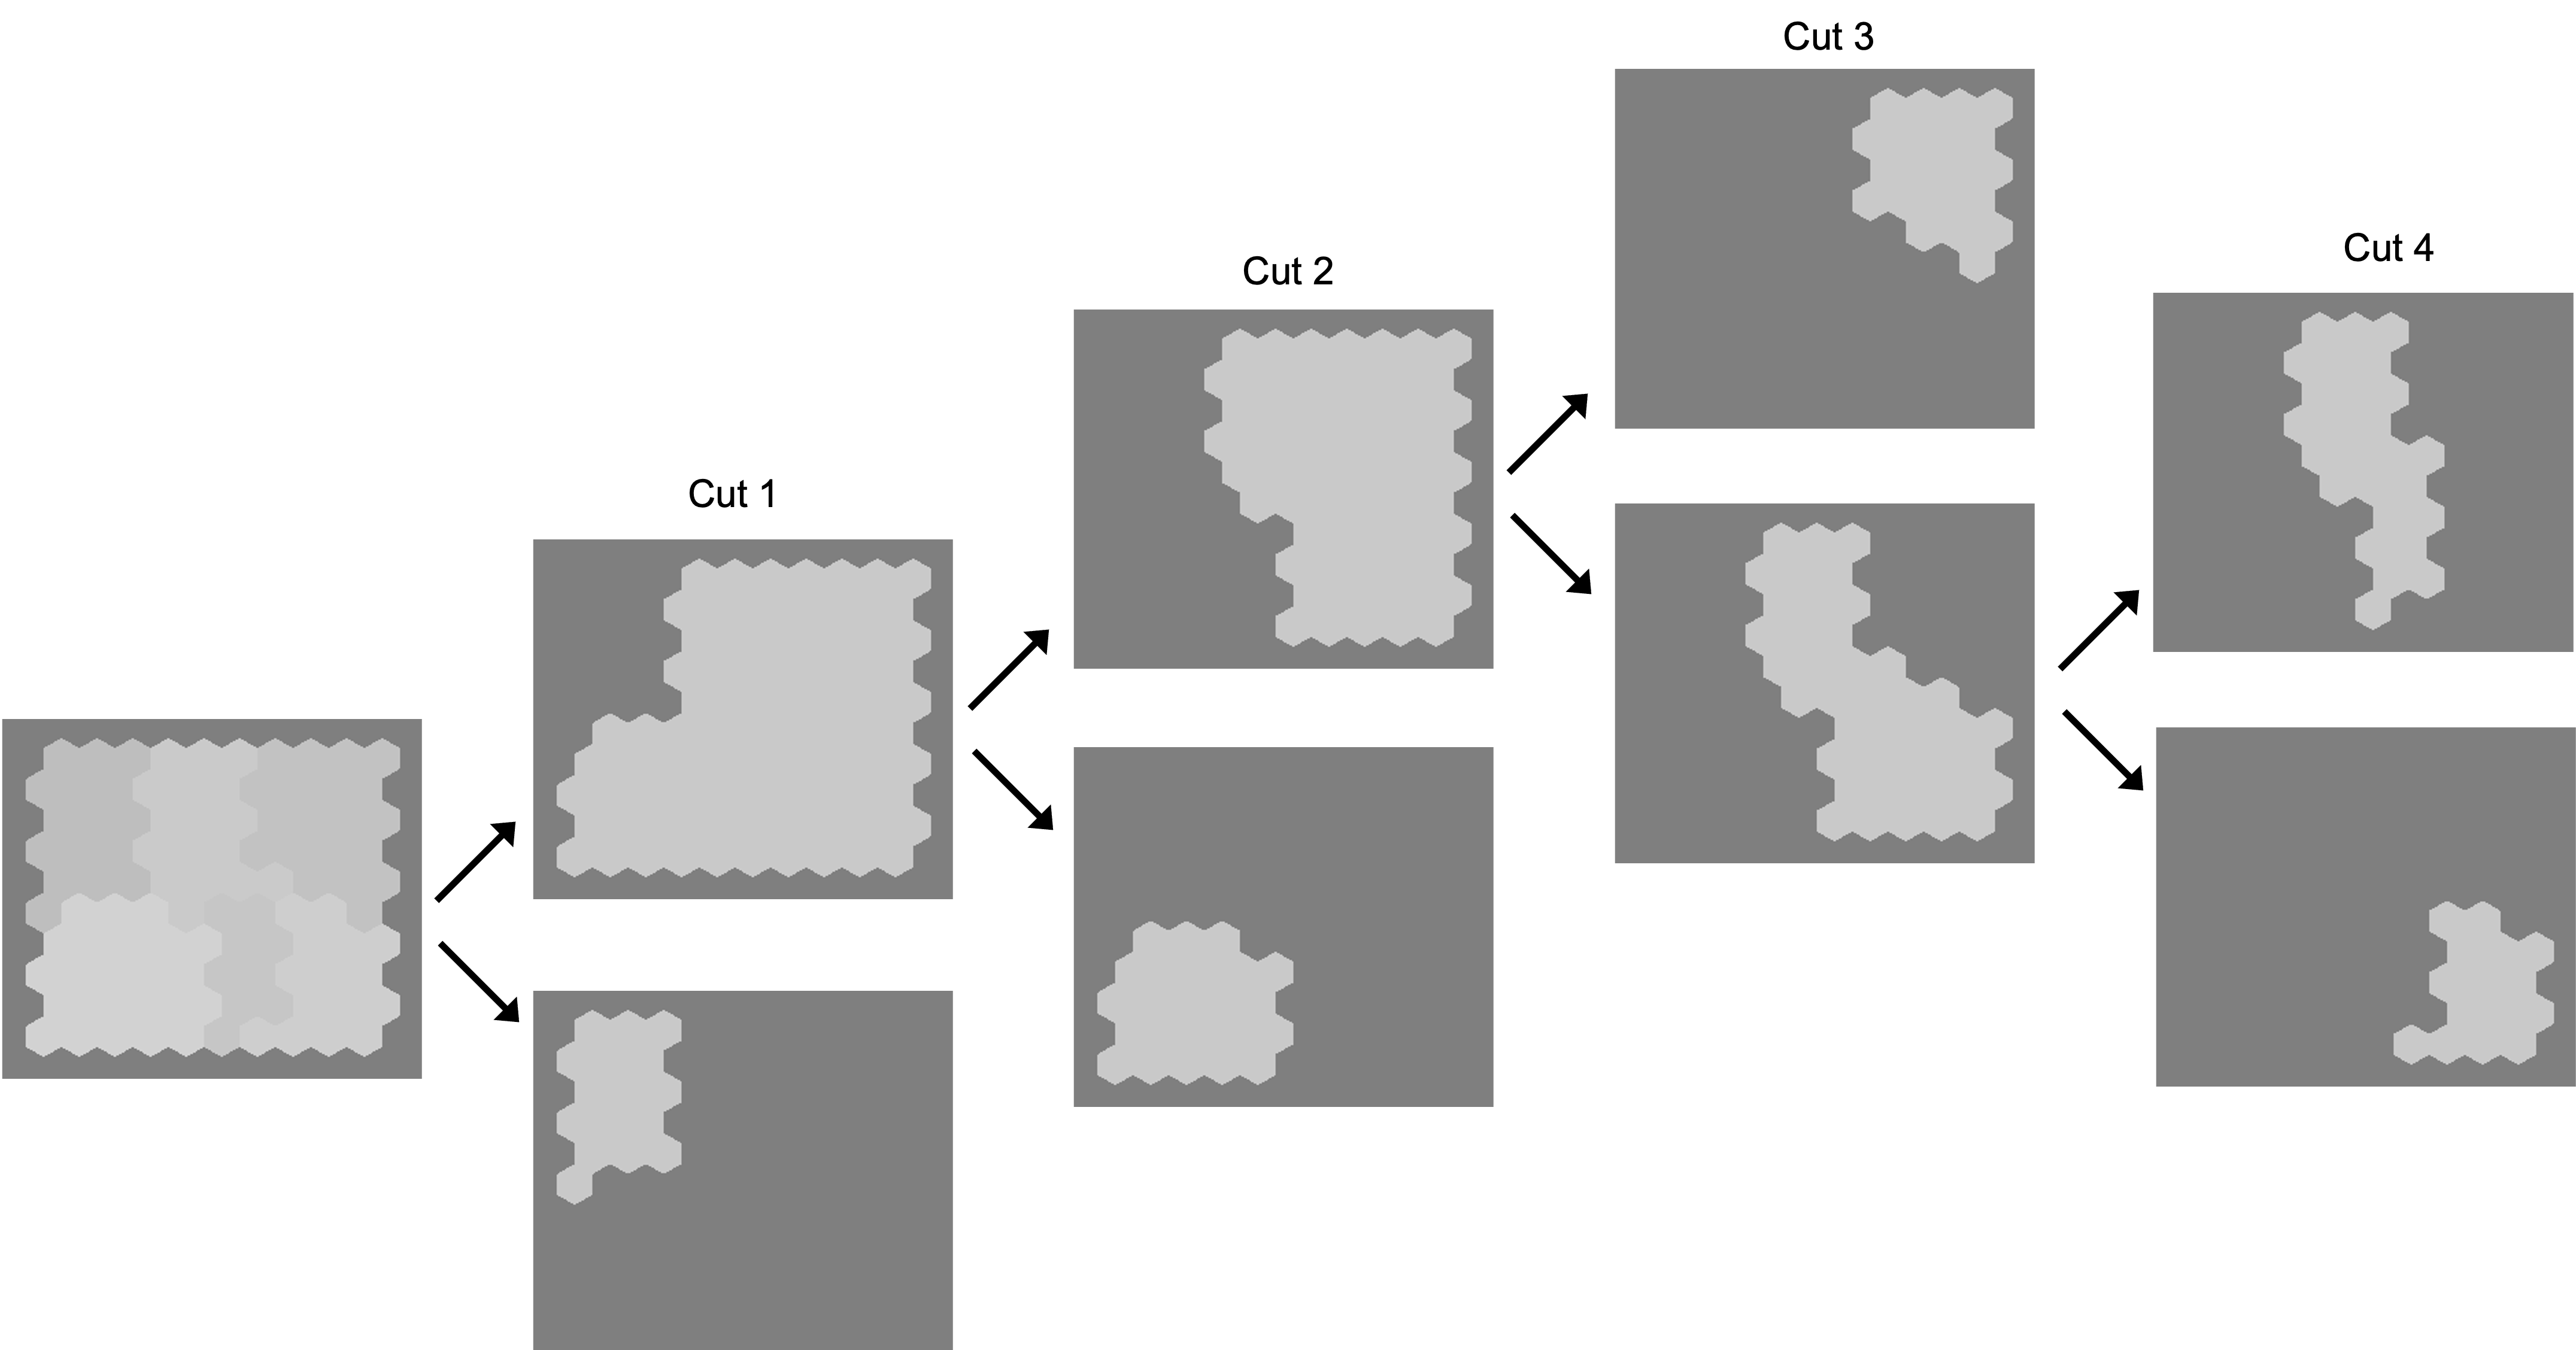
\includegraphics[width=1.1\textwidth]{pictures/segmentation_example1.png}
    \caption{First four steps of segmentation}
    \label{fig:segmentationExample1}
\end{figure}
\end{frame}

\begin{frame}{Exposure Times - Segmentation}
\begin{figure}
    \centering
    \hspace*{-0.85cm} 
    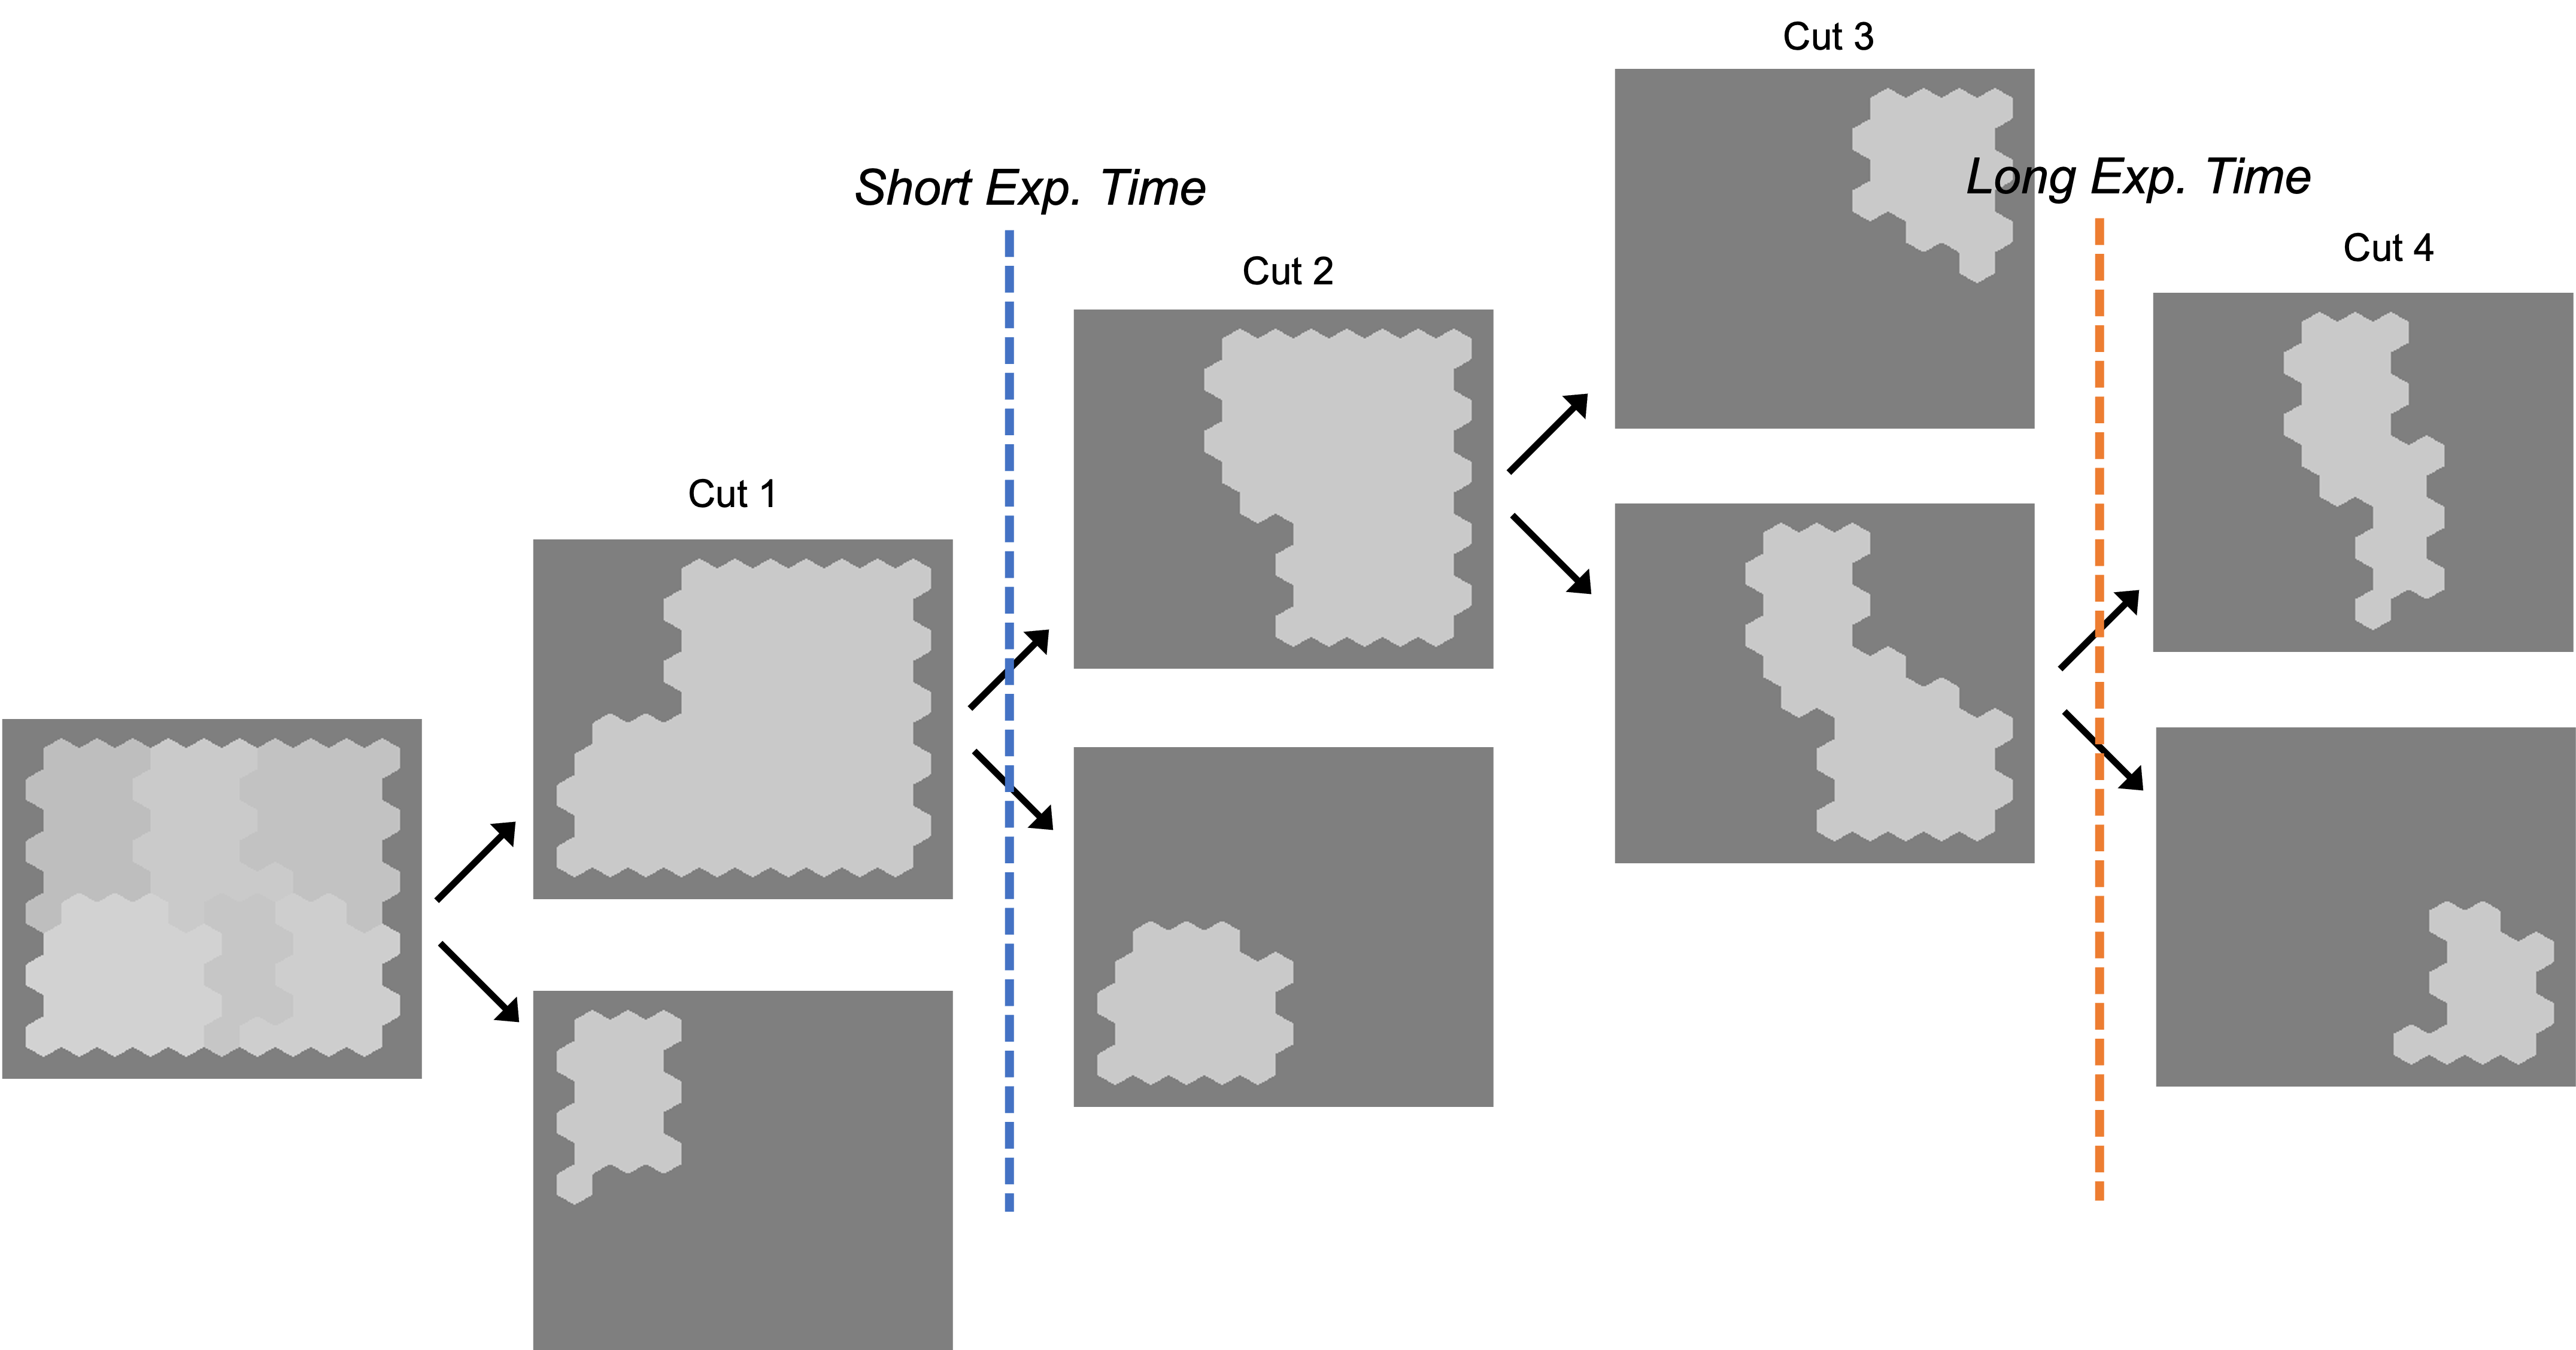
\includegraphics[width=1.1\textwidth]{pictures/segmentation_example2.png}
    \caption{First four steps of segmentation with exposure time}
    \label{fig:segmentationExample1}
\end{figure}
\end{frame}


%%%%%%%%%%%%%%%%%%%%%%%%%%%%%%%%%%%%%%%%%%%%%%%%%%
\section{Initial Results}
\begin{frame}{Small Sample Size \footnote{\footfullcite{smith2018small}}}
    \begin{itemize}
        \item Investigate systematic and functional relationship at individual participant level.
        \item Individual participant as the replication unit.
        \item Effective control of error variance
    \end{itemize}
\end{frame}

\begin{frame}{SW - Results}
    \begin{figure}
        \hspace*{-1cm} 
        \centering
        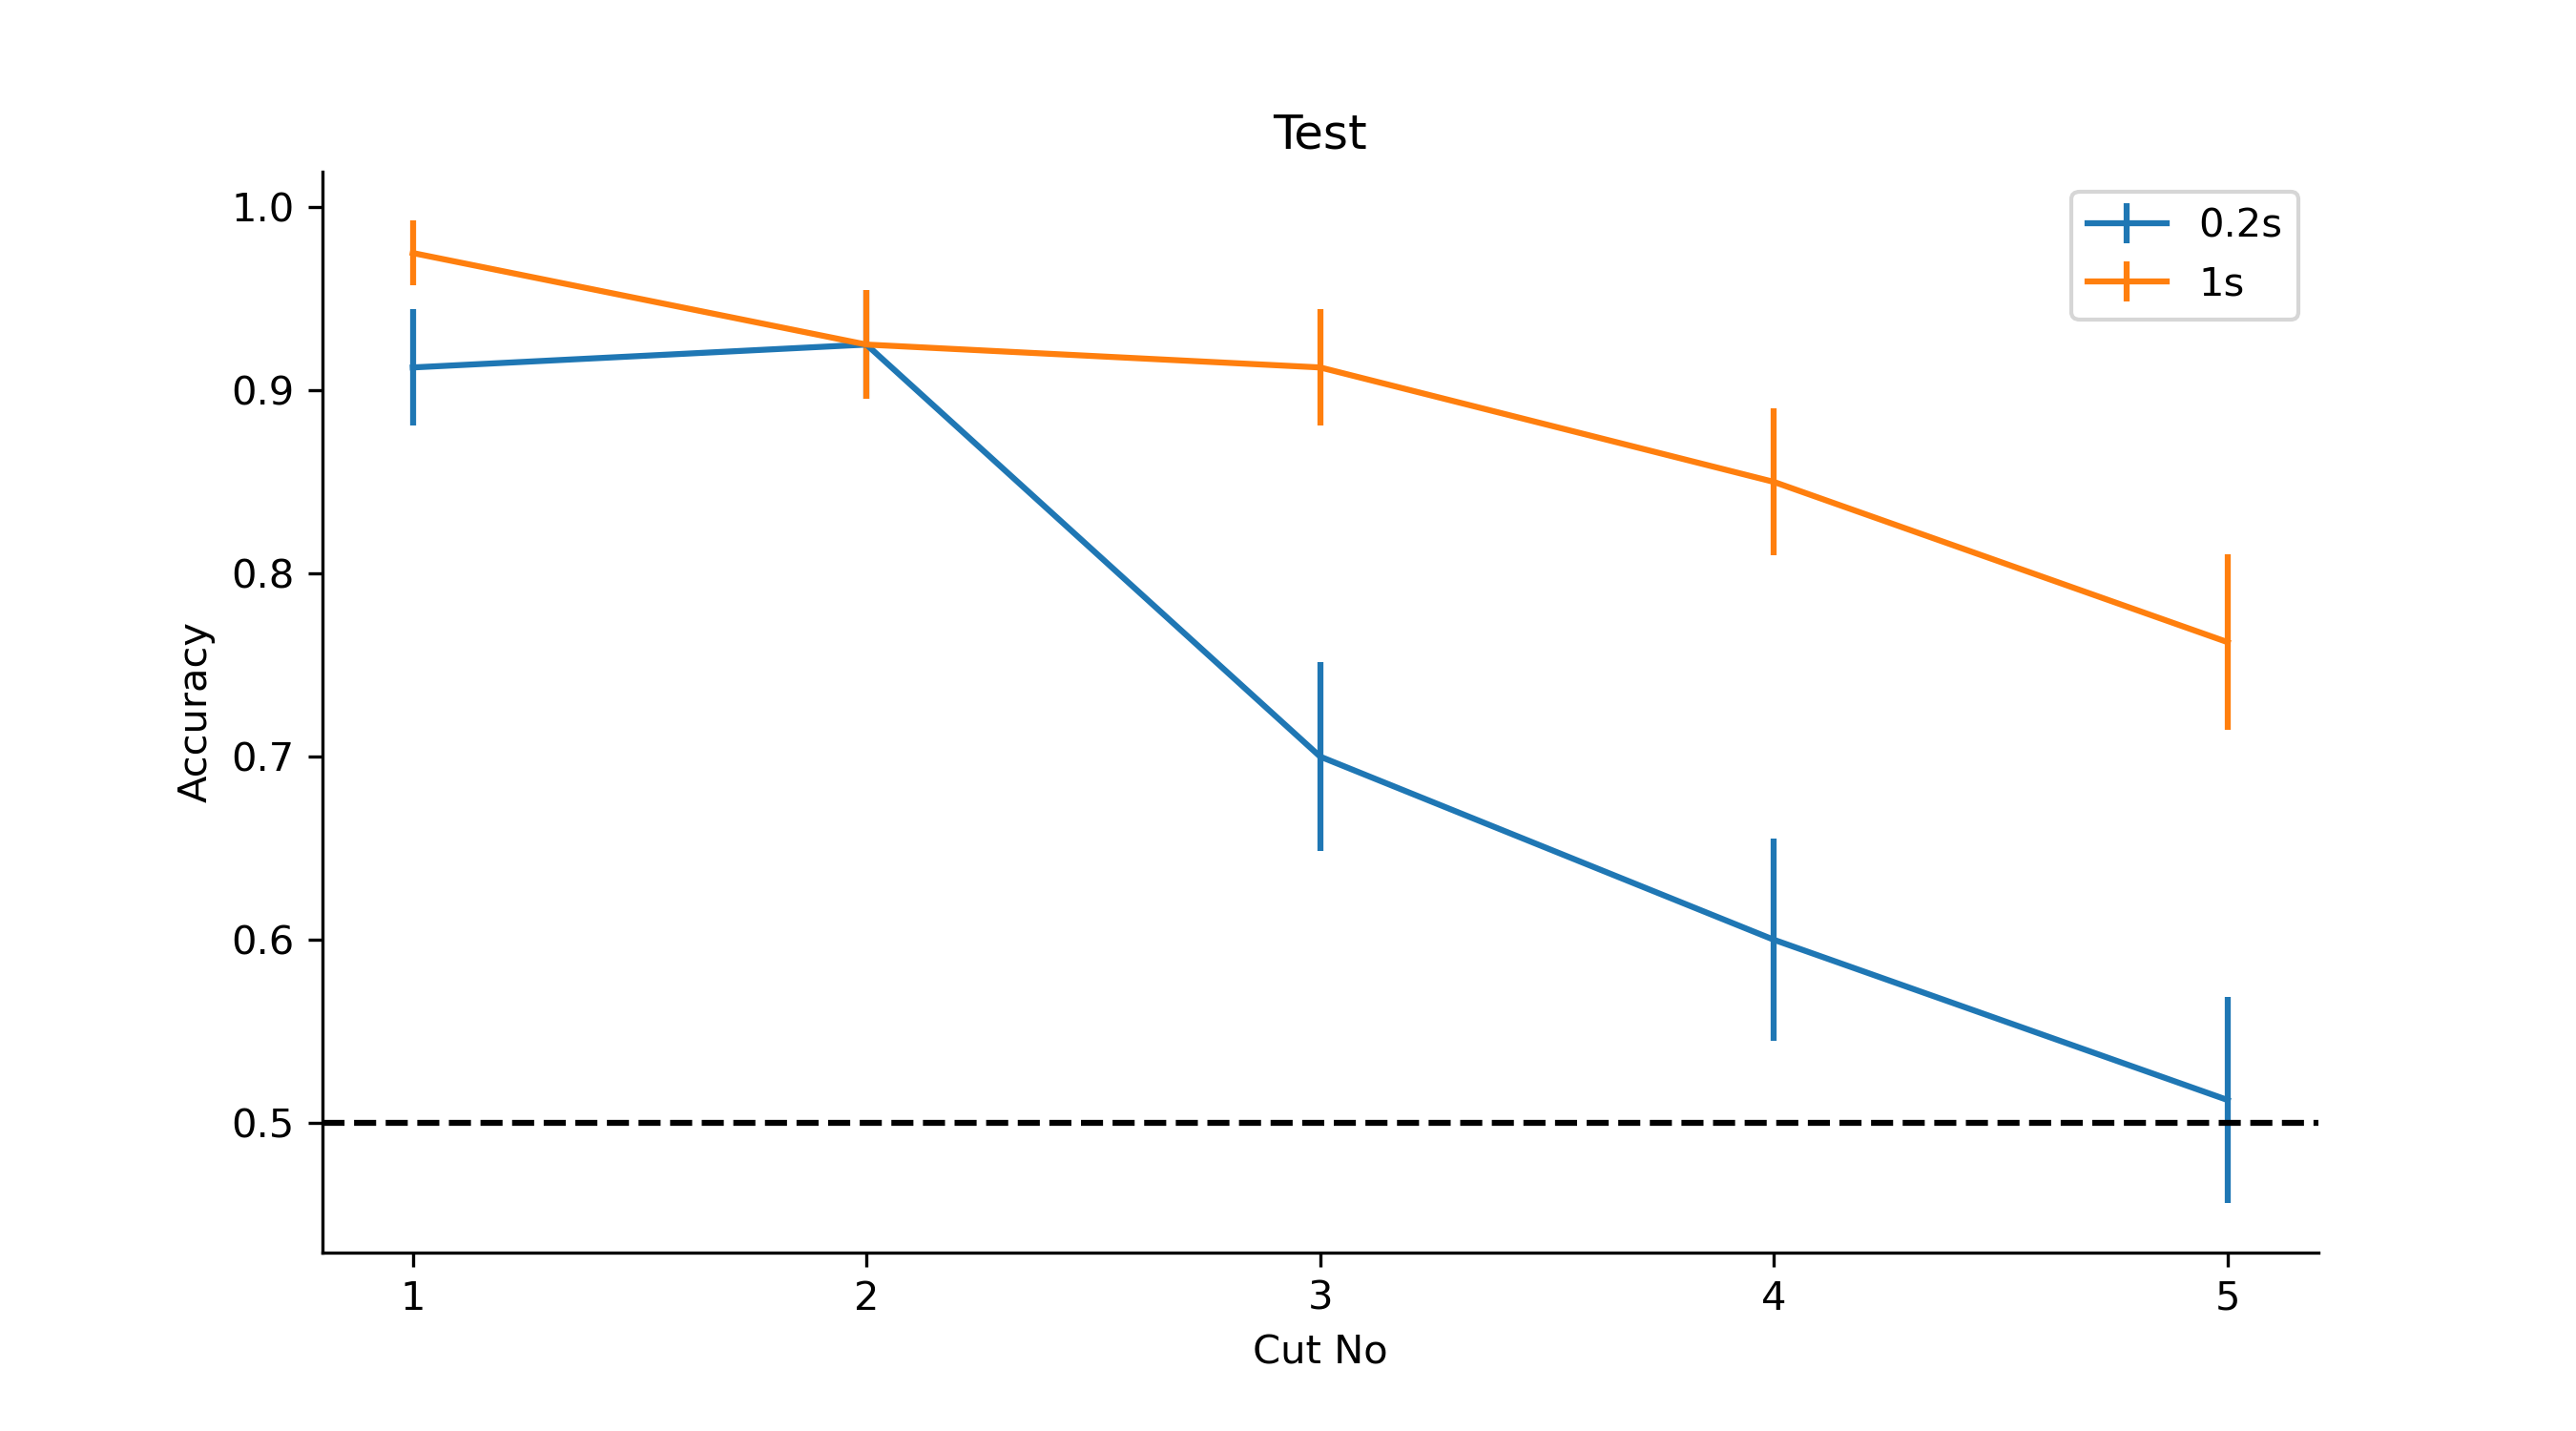
\includegraphics[width = 1.1\textwidth]{pictures/sw_test.png}
        \caption{Accuracy over cut numbers in test trials}
        \label{fig:sw_test_acc}
    \end{figure}
\end{frame}

\begin{frame}{SW - Results}
    \begin{figure}
        \hspace*{-1cm} 
        \centering
        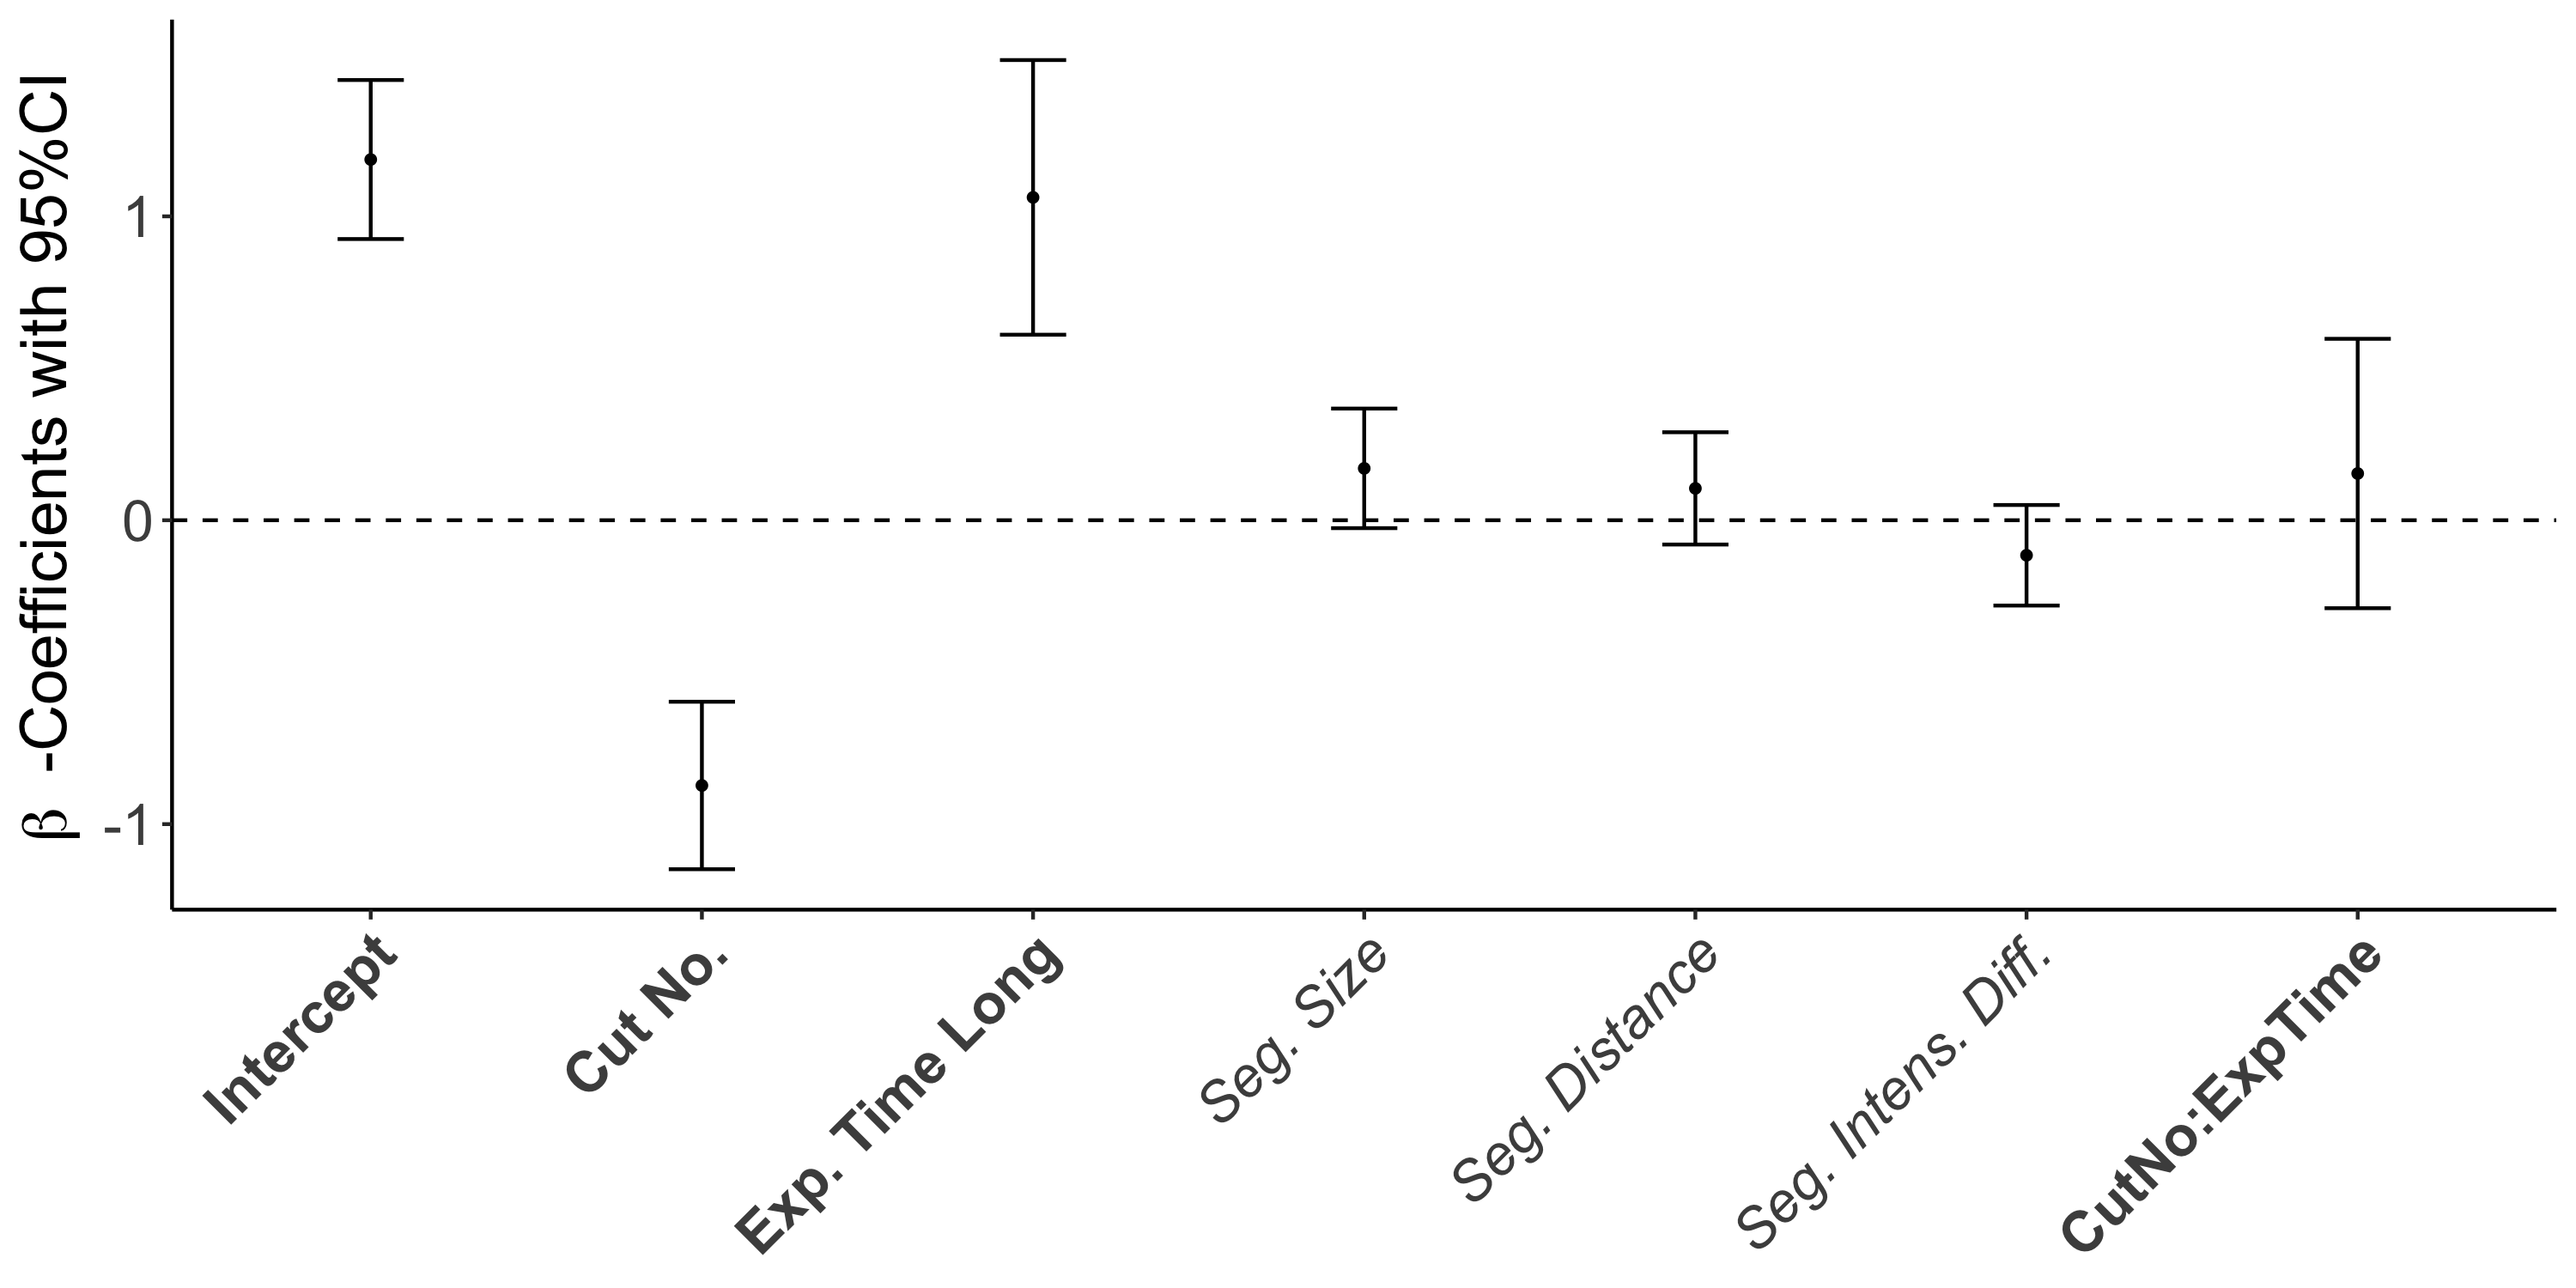
\includegraphics[width = \textwidth]{pictures/sw_test_coefficients_othrs_tgthr.png}
        \caption{Logistic regression on answers}
        \label{fig:sw_coefficients_test_othr}
    \end{figure}
\end{frame}


\begin{frame}{MY - Results}
    \begin{figure}
        \hspace*{-1cm} 
        \centering
        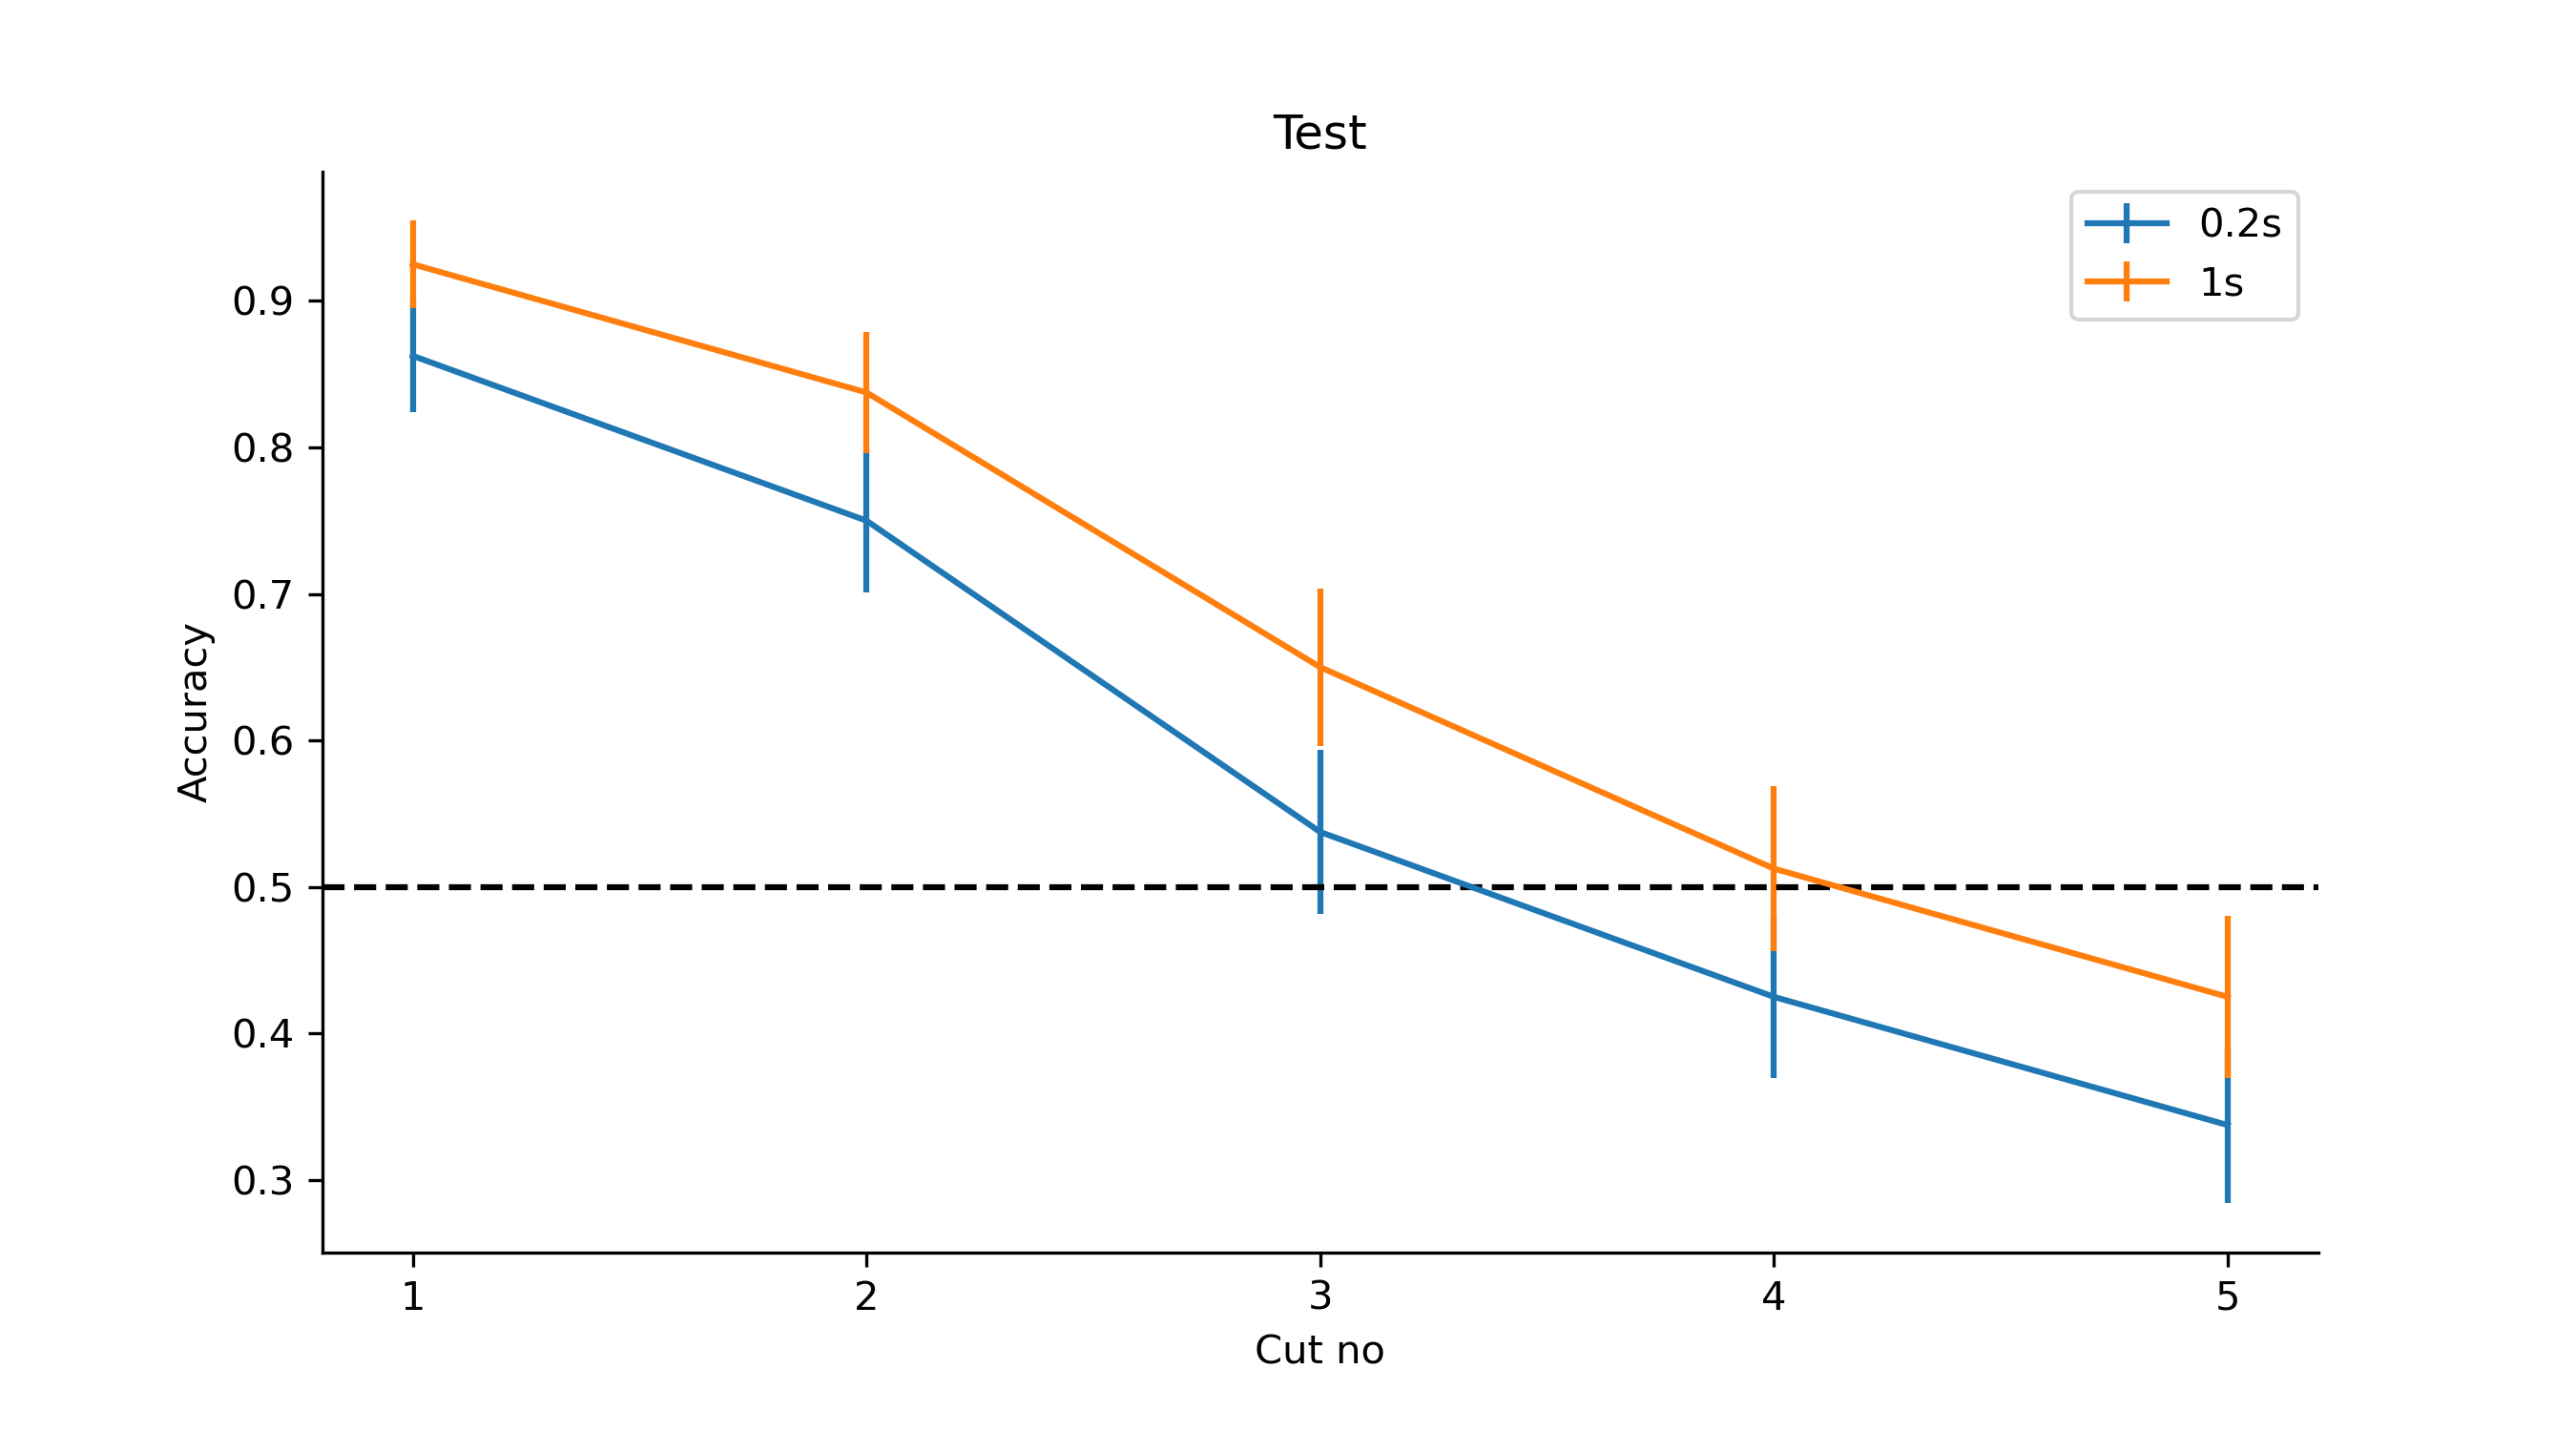
\includegraphics[width = 1.2\textwidth]{pictures/my_test.png}
        \caption{Accuracy over cut number in test trials}
        \label{fig:my_test}
    \end{figure}    
\end{frame}

\begin{frame}{MY - Results}
    \begin{figure}
        \hspace*{-1cm} 
        \centering
        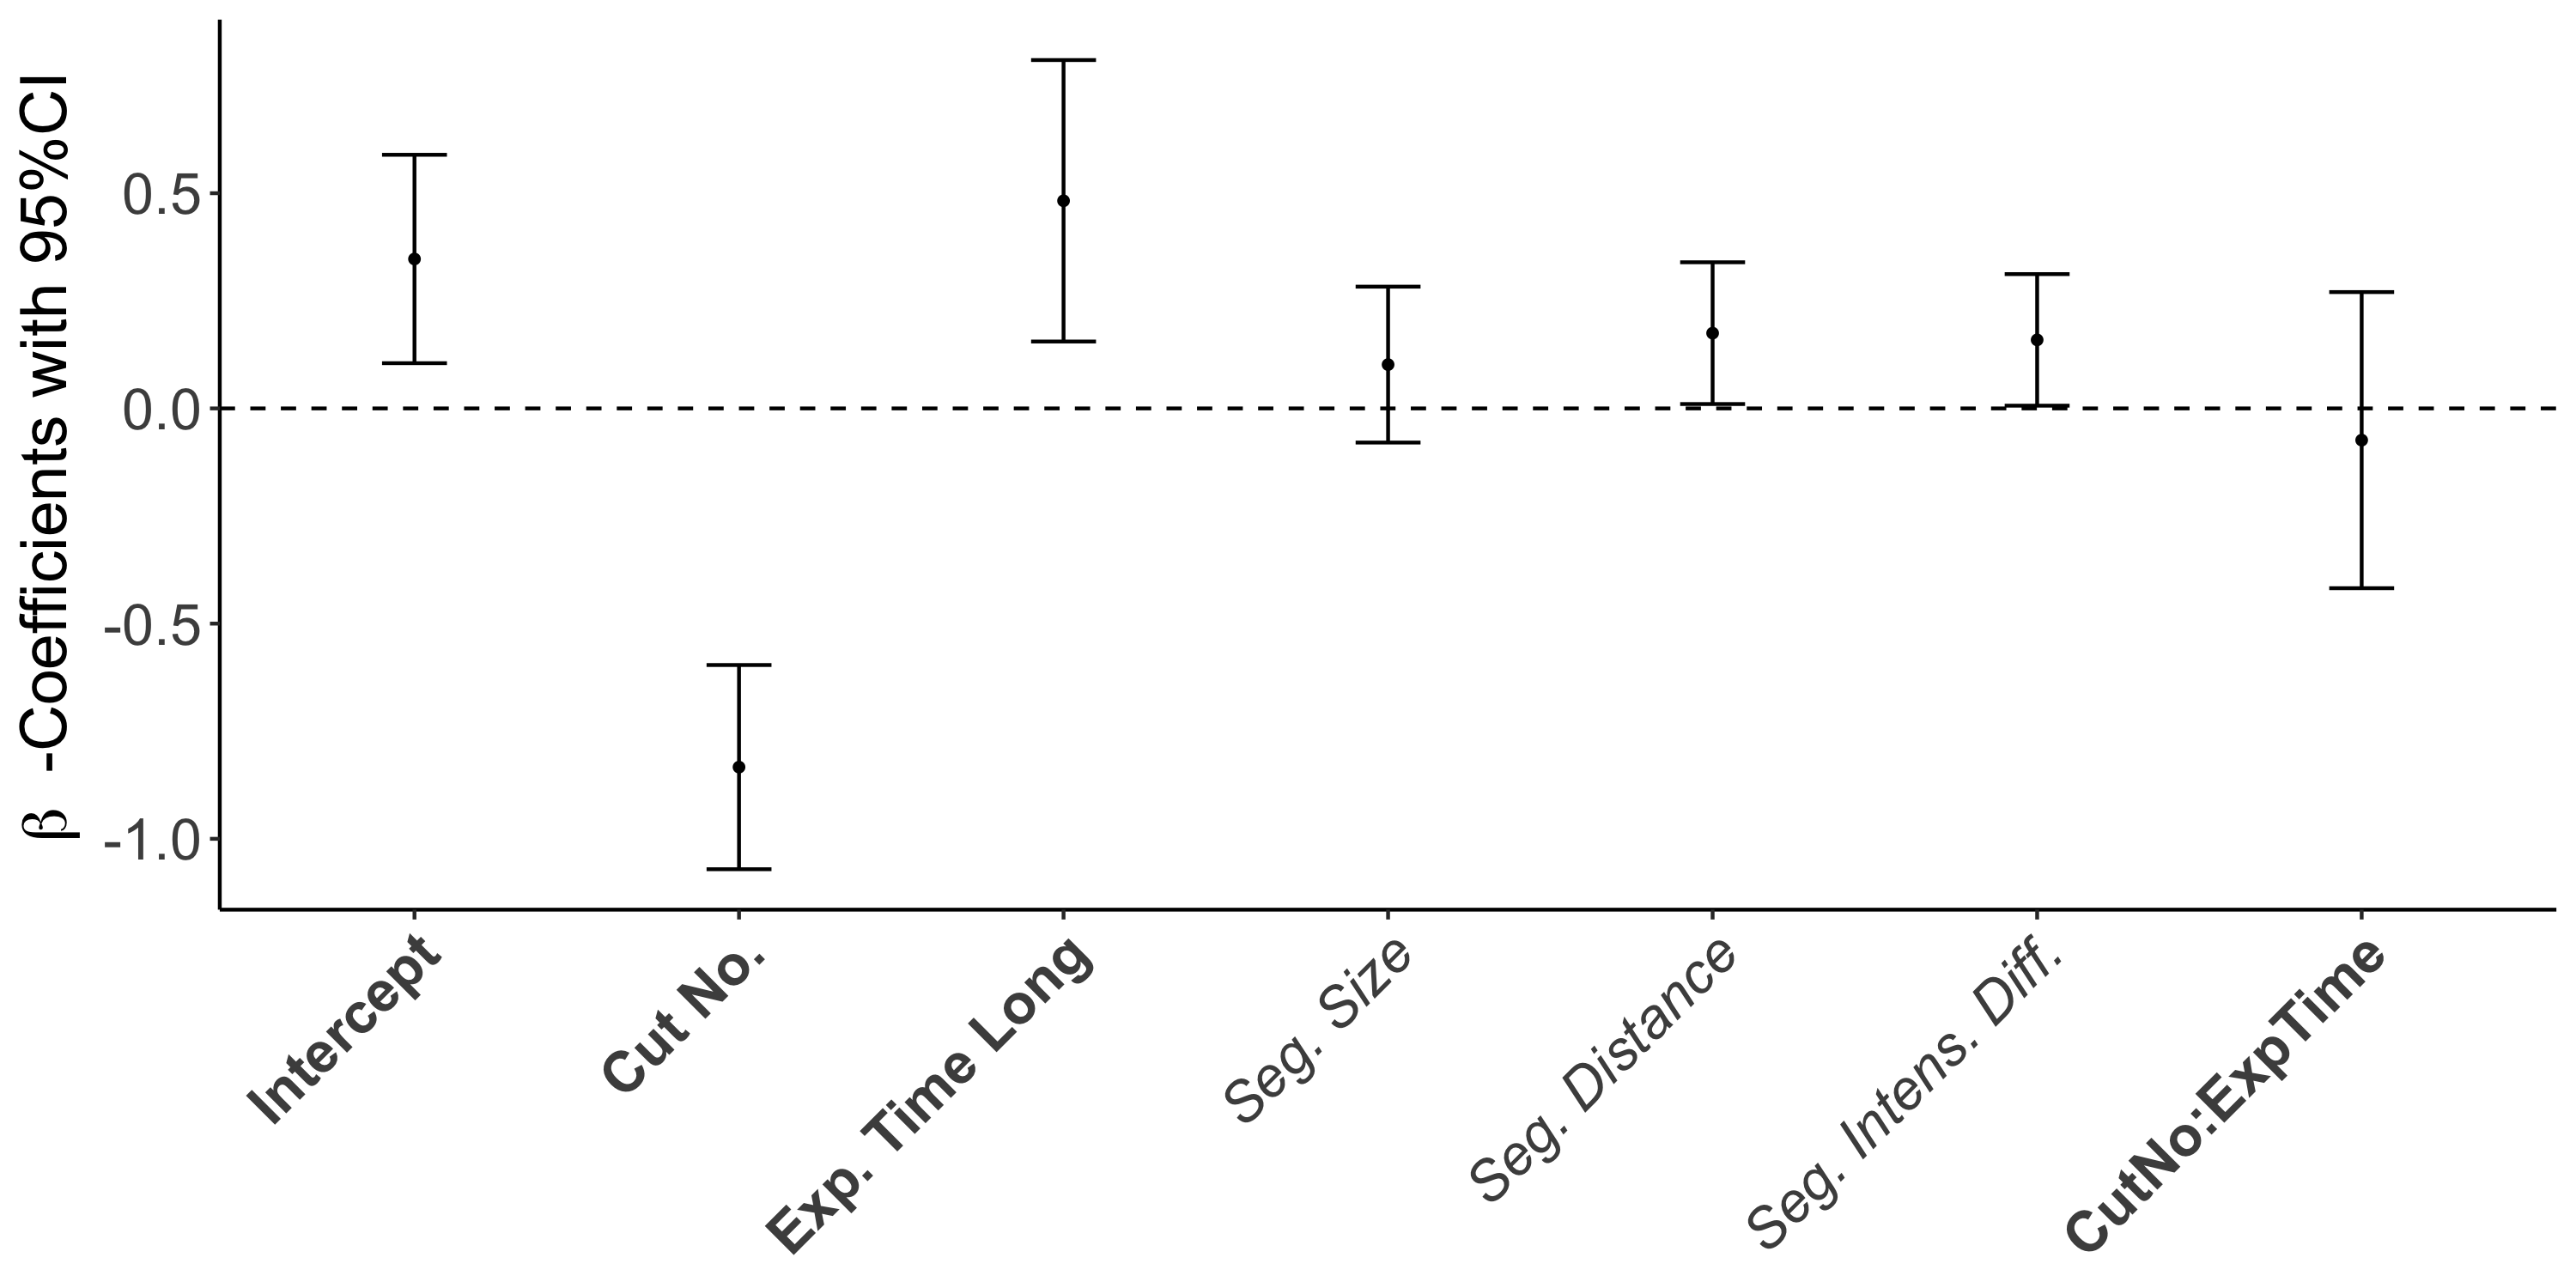
\includegraphics[width = 1.1\textwidth]{pictures/my_test_coefficients_othrs_tgthr.png}
        \caption{Logistic regression on answers}
        \label{fig:my_test_coeffs_othrs}
    \end{figure}    
\end{frame}

%%%%%%%%%%%%%%%%%%%%%%%%%%%%%%%%%%%%%%%%%%%%%%%%%%
\section{Summary and Further Directions}
\begin{frame}{Summary}
    \metroset{block=fill}
    \begin{exampleblock}{\textsc{Hypothesis}}
        As more computational resources are allocated, perceptual grouping behavior gets refined and finer segments can be detected.
    \end{exampleblock}

    \begin{itemize}
        \item Evidence for hierarchical segmentation
        \item Finding finer structures requires more resources
        \item We found exposure time has positive effect on finding finer segments in the image
    \end{itemize}
\end{frame}

\begin{frame}{Further Directions}
    \begin{itemize}
        \item Collect data from naïve participants
        \item Modelling responses for control trials
        \item Modelling errors using similarity
        \begin{enumerate}
            \item Intensity difference
            \item Cut order
            \item Border similarity
        \end{enumerate}
    \end{itemize}
\end{frame}


\begin{frame}{Questions}
    \centering
    \huge Thank You! \\
    \huge Questions?
\end{frame}

\begin{frame}{Representing Images with Graph Networks}
\begin{itemize}
    \item Assign weights to each edge.
    \item The weights represent the similarity of two pixels.
\end{itemize}
\begin{align}
w_{ij} = e^{\dfrac{-||F_{(i)} - F_{(j)}||_2^2}{\sigma_I^2}}
*
    \begin{cases}
    e^\dfrac{-||X_{(i)} - X_{(j)}||_2^2}{\sigma_X^2}, &  \text{if } ||X_{(i)} - X_{(j)}||_2 < r\\
    0,                                               &  \text{otherwise}
    \end{cases}
\end{align}
\\
  \pause
  -   $F$ is feature vector based on \textbf{brightness}, color, texture, or motion information. \\
  \pause
  -   $r$ is distance between two pixel nodes $i$ and $j$. \\ 
  -   $w_{ij} = 0$ when $i$ and $j$ are apart more than $r$ \\
  -   As $\sigma_I$ gets larger, the differences between the weights decrease \\
\end{frame}

\begin{frame}{Generating Images}
\begin{columns}
    \column{0.6\textwidth}
    \vspace{-1cm}
    \begin{enumerate}
        \item 10 x 10 grid pattern made of hexagons.
        \vspace{1.5cm}
        \item Assign 6 equally distant seed on the grid. 
        \vspace{1.5cm}
        \item Sample a variance from a normal distribution and add to the seed coordinates.
    \end{enumerate}
    \column{0.4\textwidth}
    \vspace{-0.25cm}
    \begin{figure}
        \centering
        
\includegraphics[width=0.8\textwidth]{pictures/img3_cut0.png}
    \end{figure}
    \vspace{-0.7cm}
    \begin{figure}
        \centering
        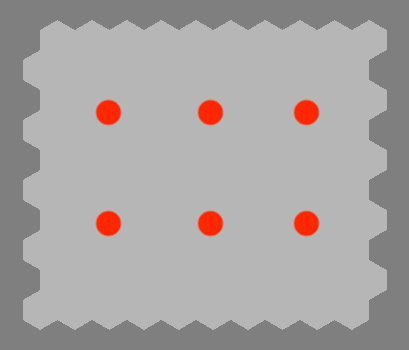
\includegraphics[width=0.8\textwidth]{pictures/img3_cut0_seeds.png}
    \end{figure}
    \vspace{-0.7cm}
    \begin{figure}
        \centering
        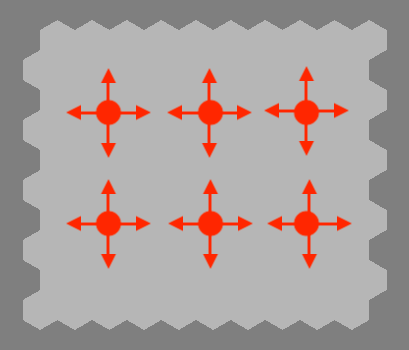
\includegraphics[width=0.8\textwidth]{pictures/img3_cut0_seeds_var.png}
    \end{figure}
\end{columns}
\end{frame}

\begin{frame}{Generating Images}
\begin{columns}
    \column{0.6\textwidth}
    \begin{enumerate}
        \setcounter{enumi}{3}
        \vspace{-0.5cm}
        \item Establish regions for each one of the seeds using Voronoi Diagram.
        \vspace{2cm}
        \item Map each of the groups to intensity values.
    \end{enumerate}
    \column{0.4\textwidth}
    \begin{figure}
        \centering
        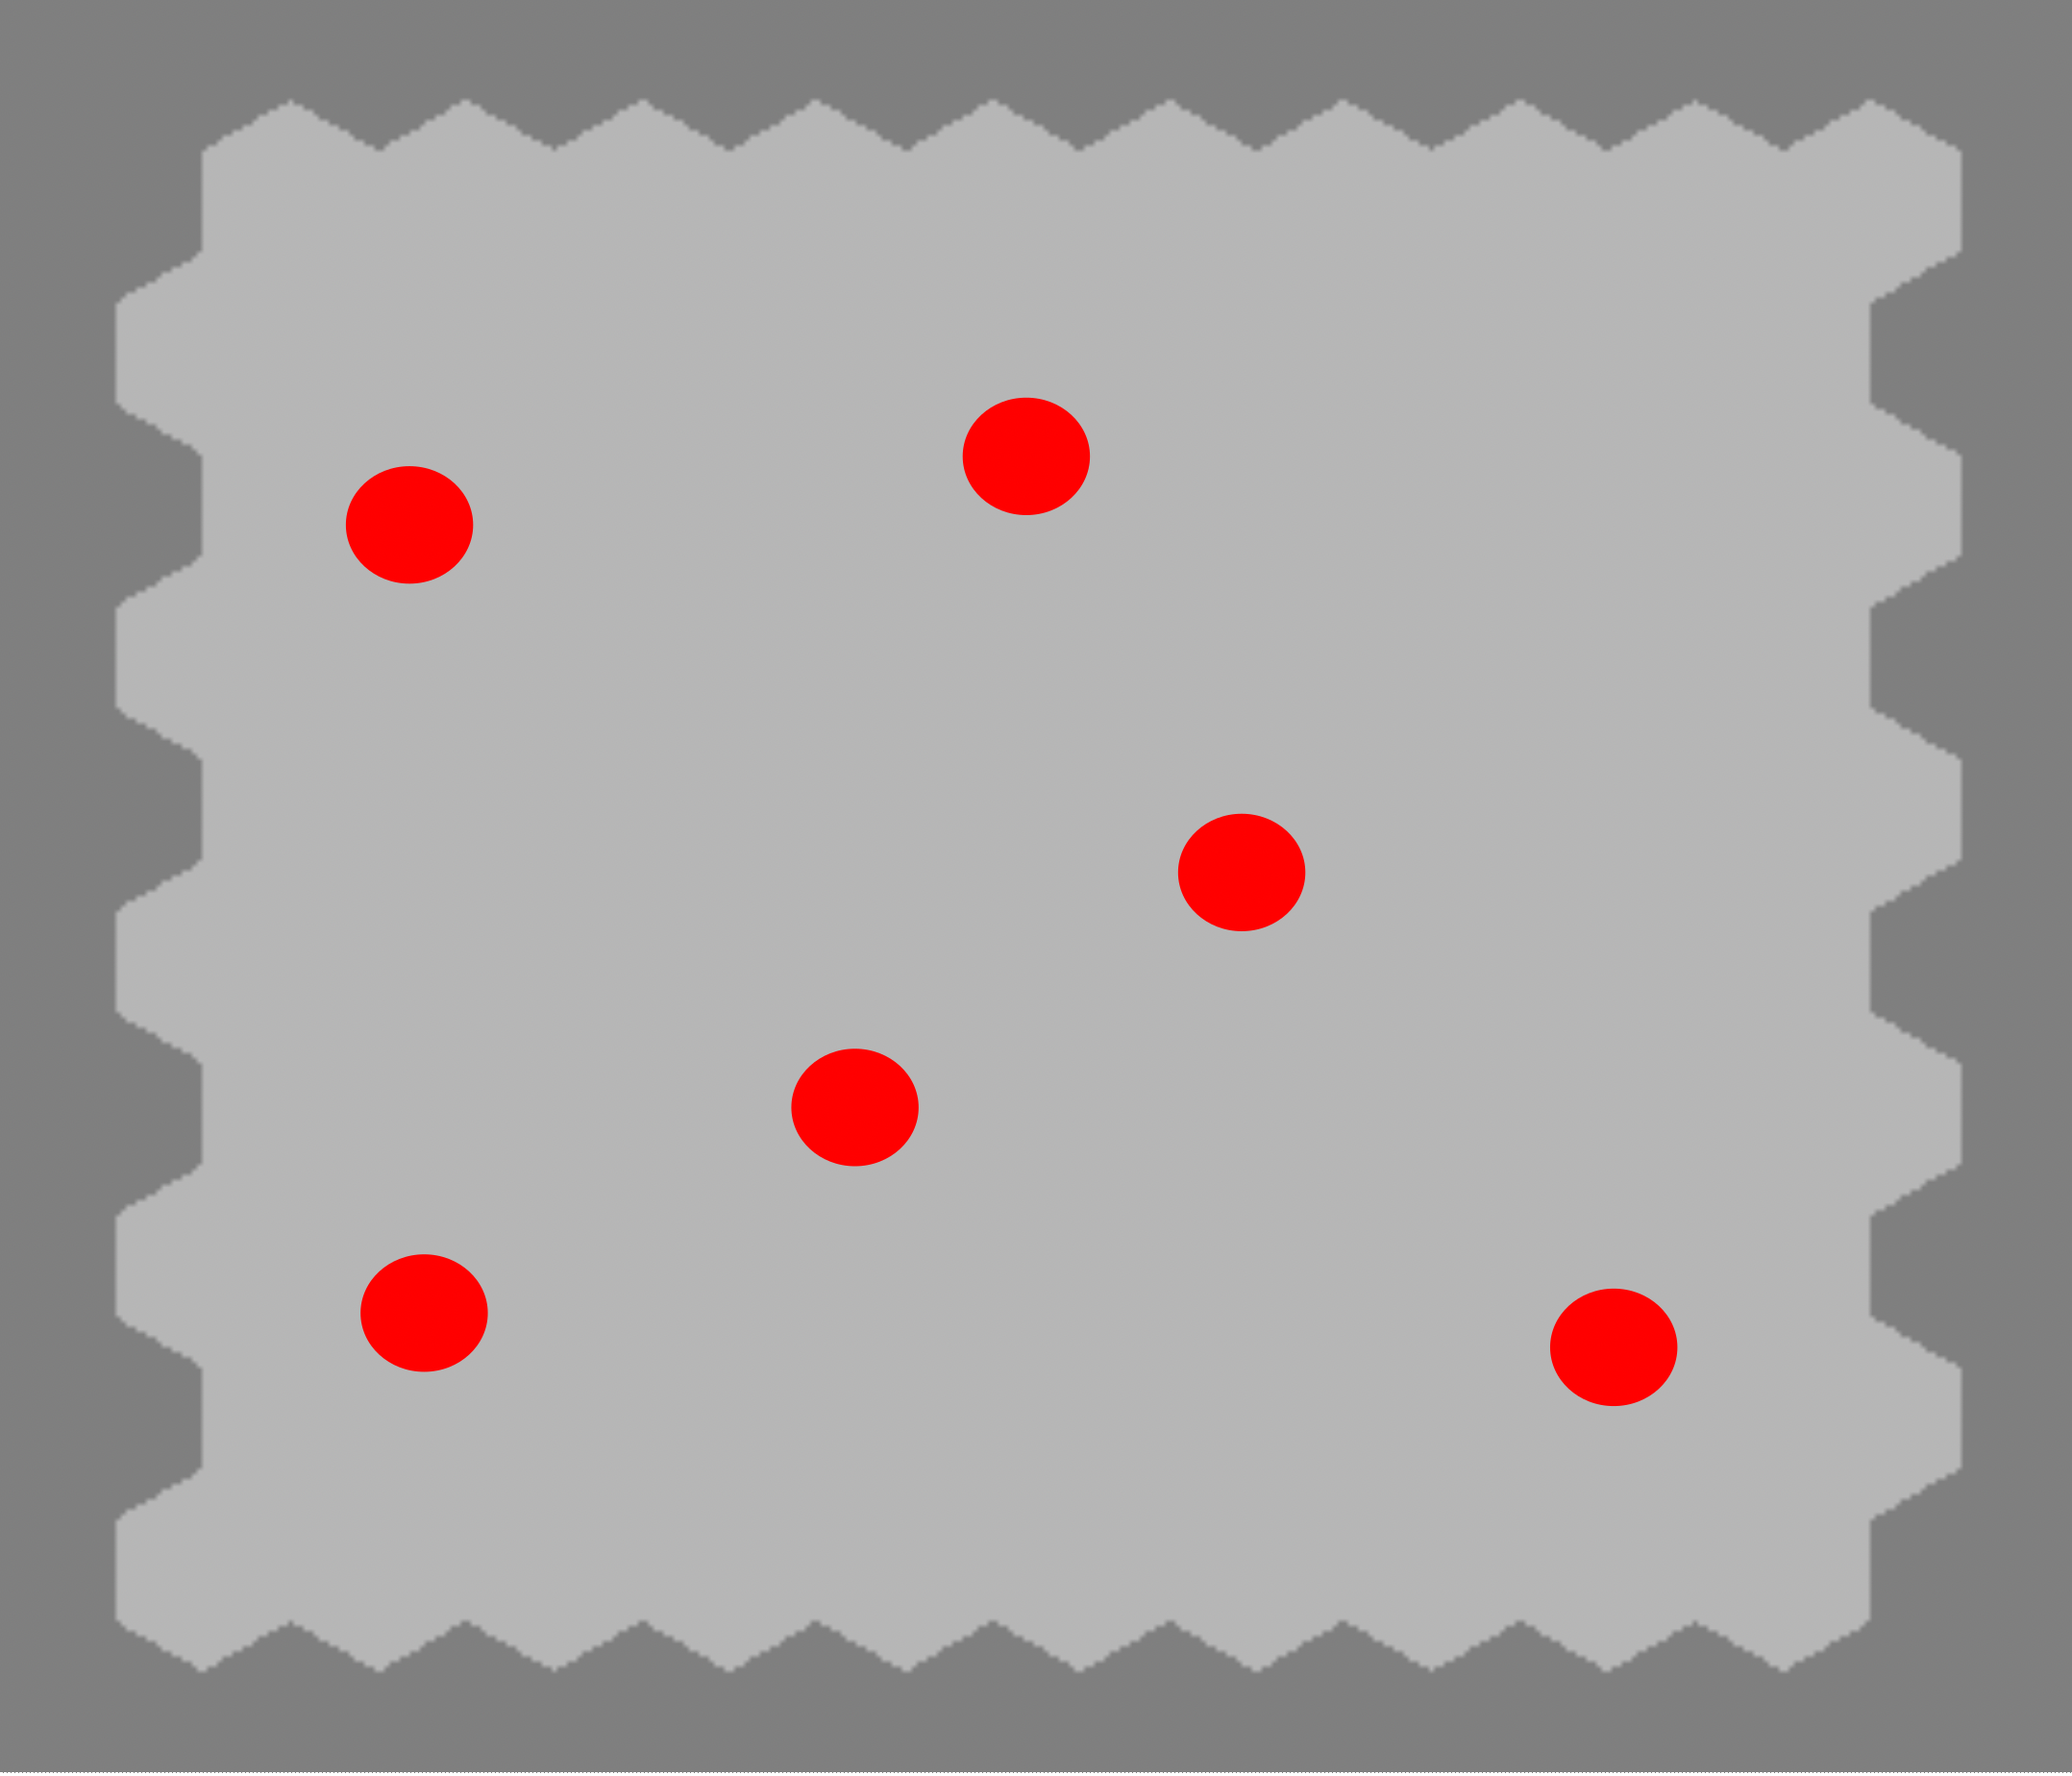
\includegraphics[width=0.8\textwidth]{pictures/img3_cut0_seed_final.png}
    \end{figure}
    \vspace{-0.62cm}
    \begin{figure}
        \centering
        
\includegraphics[width=0.8\textwidth]{pictures/intensities.png}
    \end{figure}
    \vspace{-0.6cm}
    \begin{figure}
        \centering
        
\includegraphics[width=0.8\textwidth]{pictures/grid_init3.png}
    \end{figure}
\end{columns}
\end{frame}

\begin{frame}{Getting Segments}
        We need to find an algorithm that:
        \begin{itemize}
            \item Detects global segments prior to local segments.
            \item Has hierarchical structure.
            \item Represents the computational resources spent on the segmentation process.
        \end{itemize}
\end{frame}

\begin{frame}{Pilot - Exposure Times}
    \begin{figure} 
        \hspace*{-0.5cm}
        \centering
        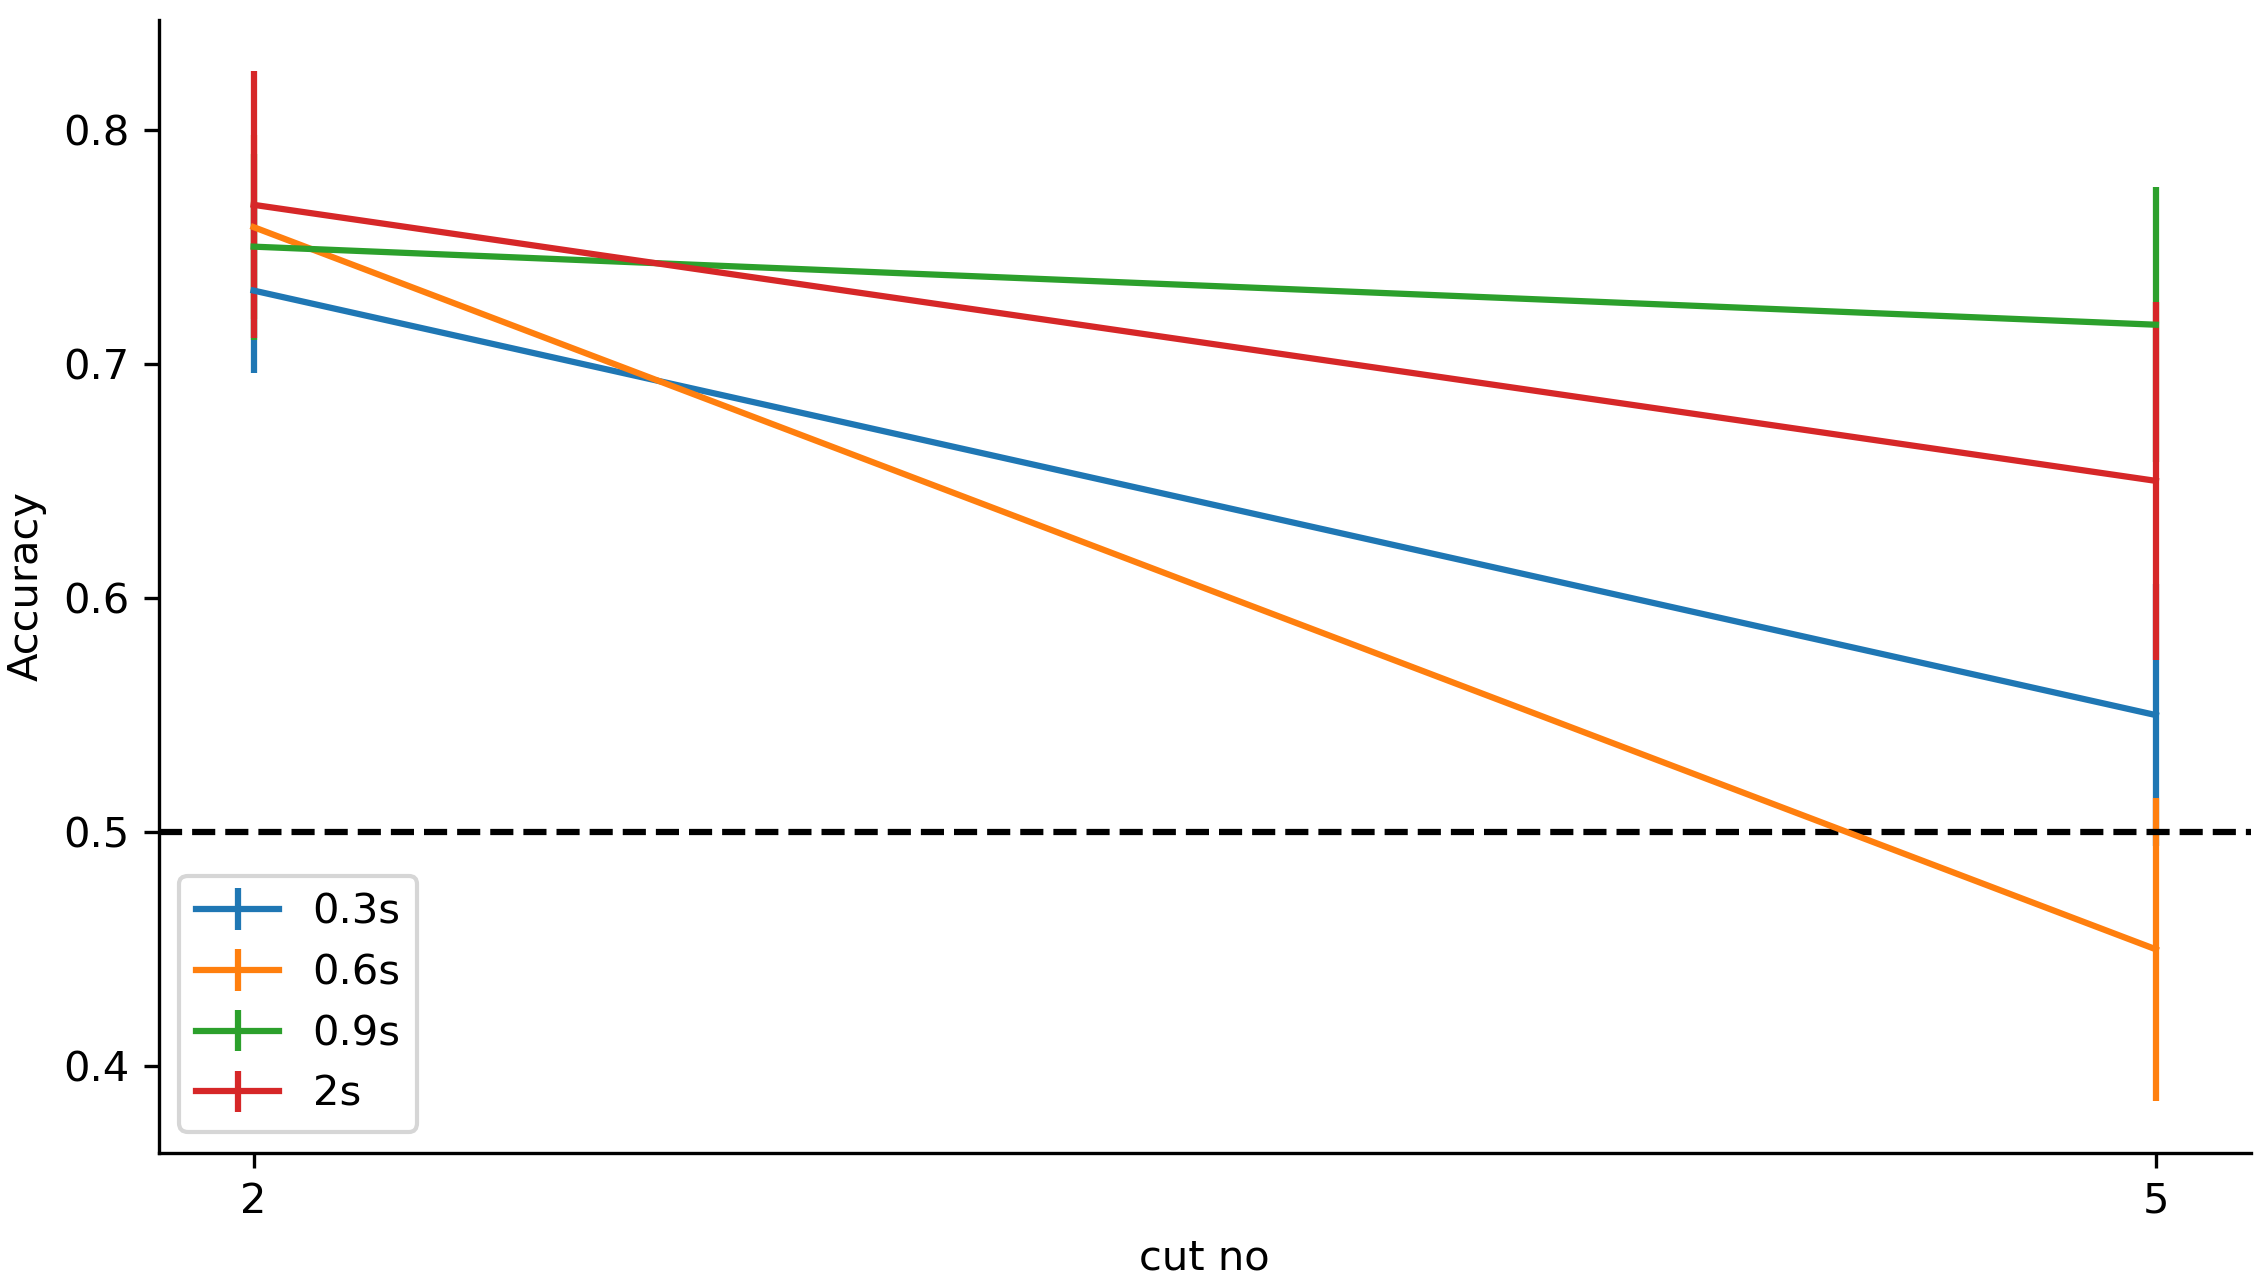
\includegraphics[width=0.9\textwidth]{pictures/ExpTimeComparison.png}
        \caption{Comparison of different exposure times}
        \label{fig:comp_exposure_times}
    \end{figure}
    
    \begin{itemize}
        \item We can detect first two segments in 300 ms
        \item After 900ms, performance decreases in cut no 5
    \end{itemize}
\end{frame}


\begin{frame}{SW - Control Results}
    \begin{figure}
        \hspace*{-1cm} 
        \centering
        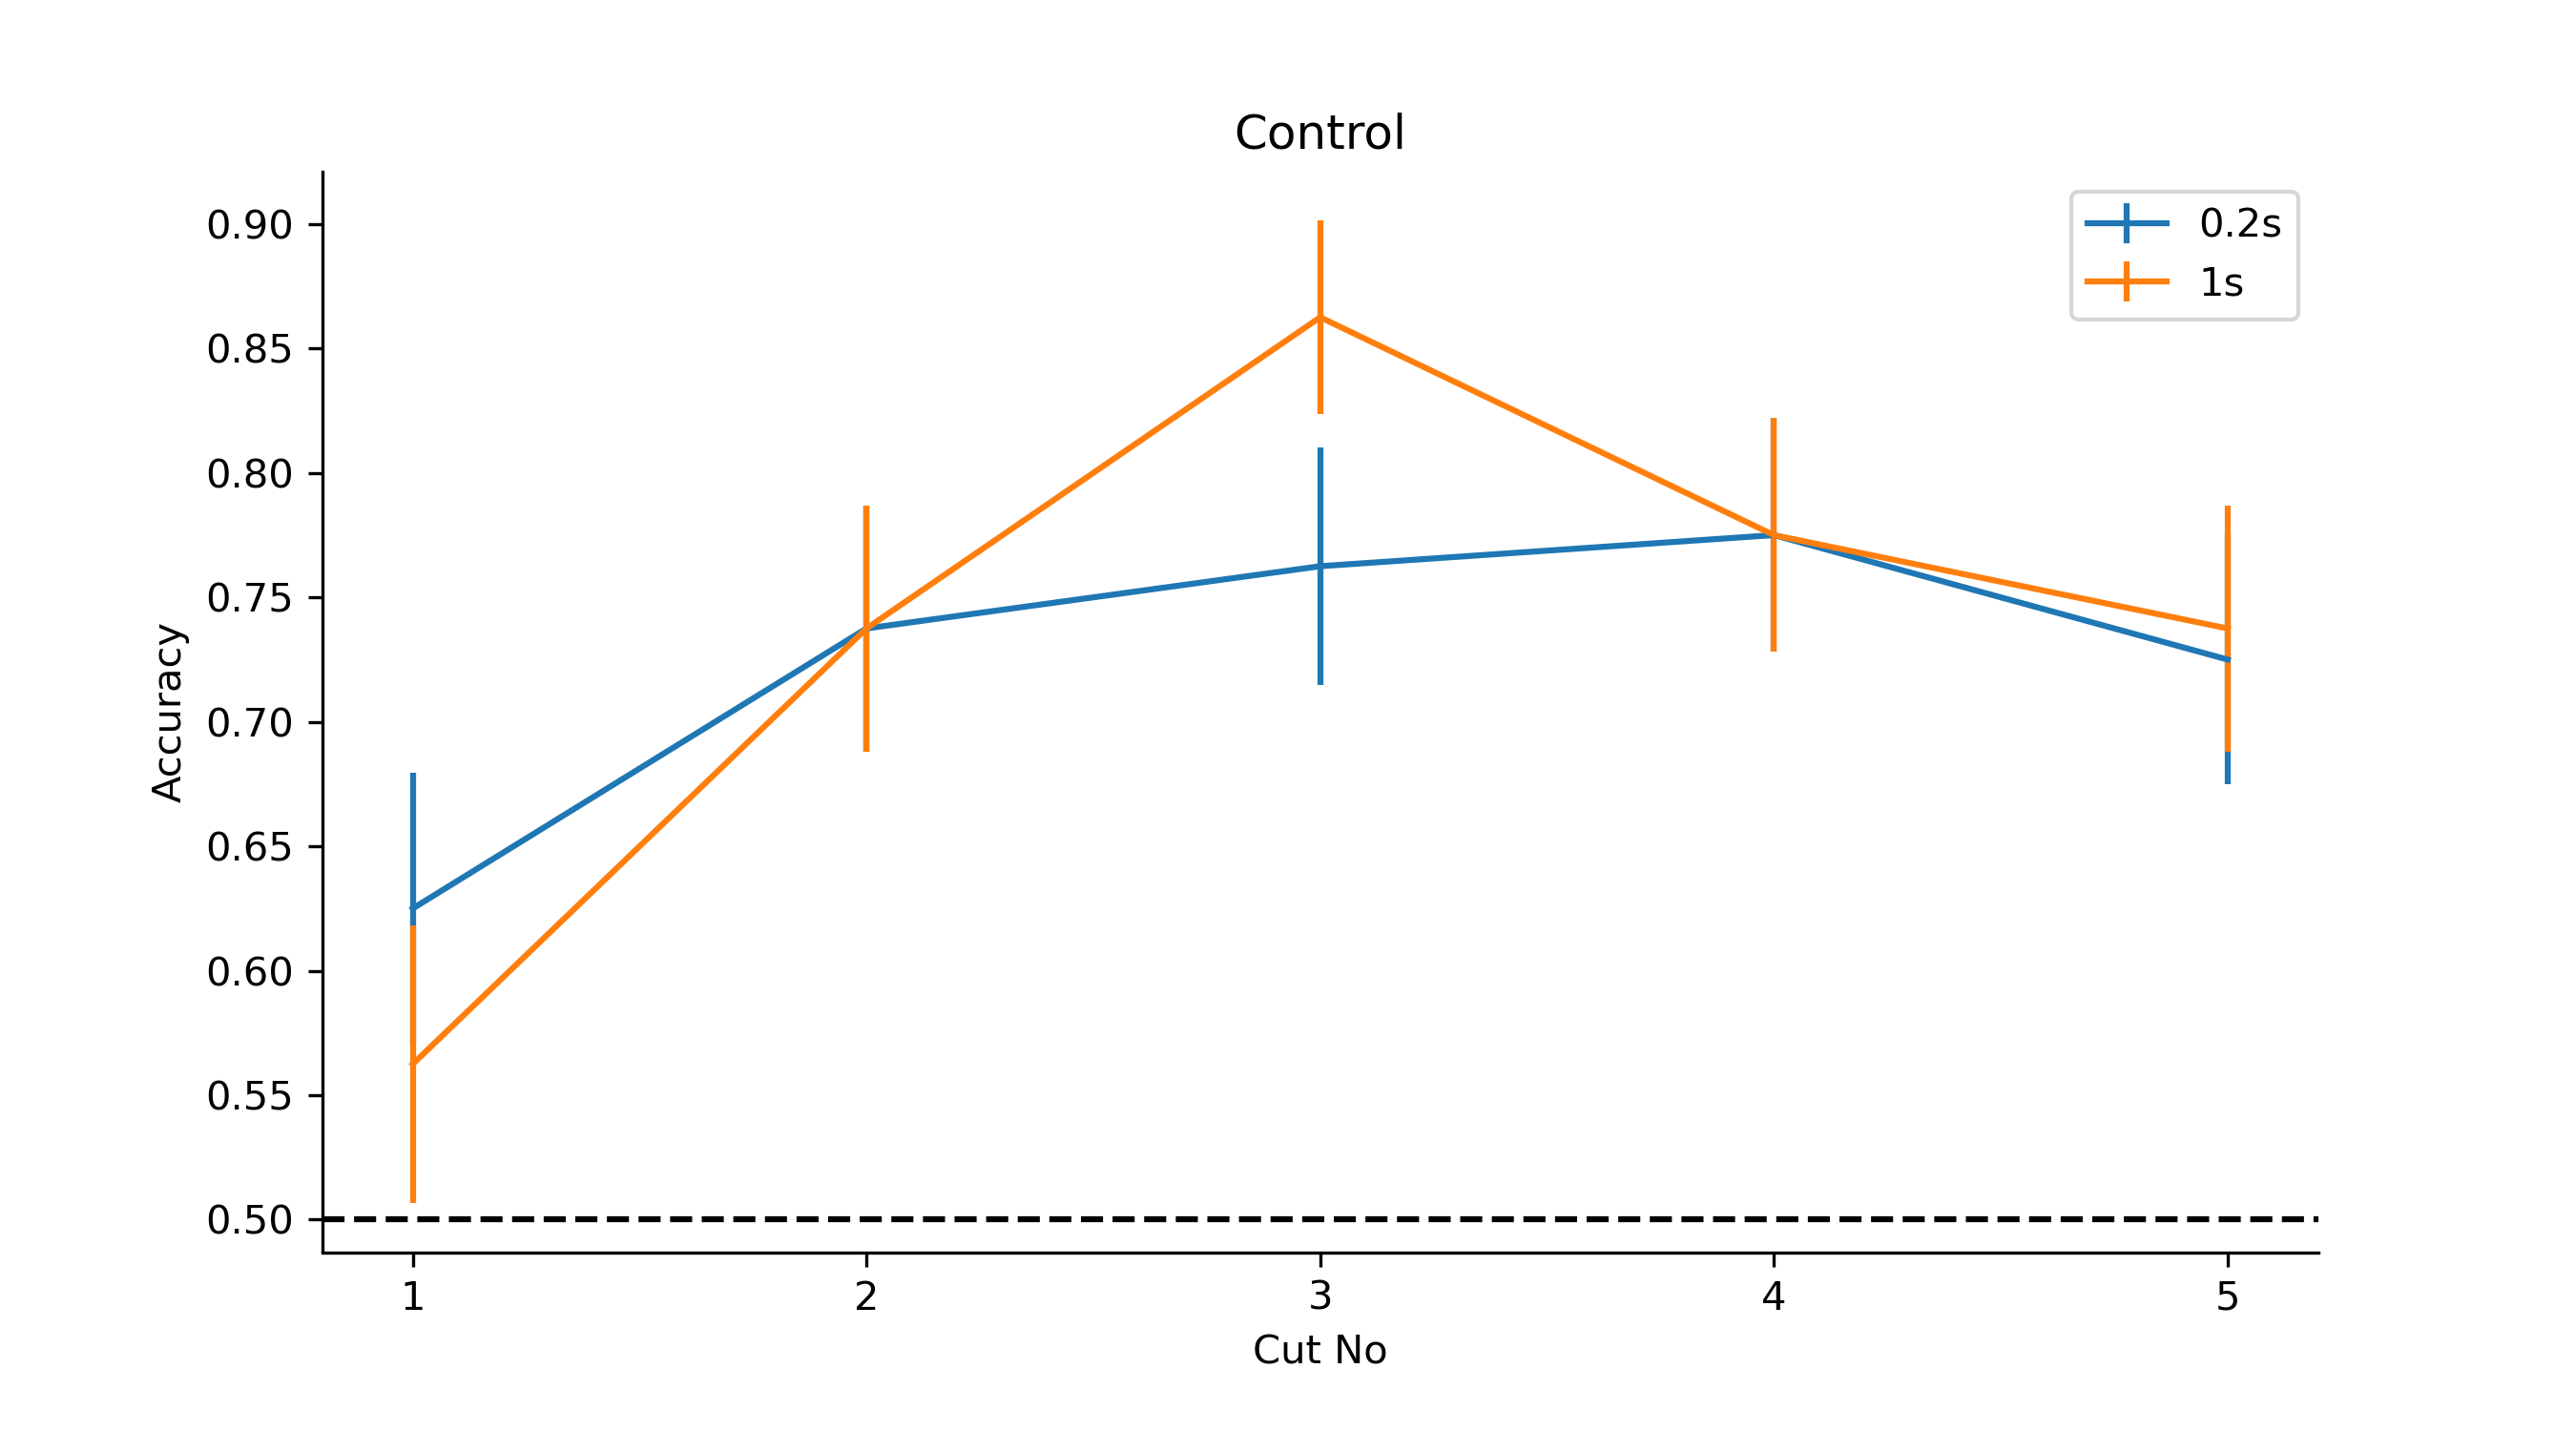
\includegraphics[width = 1.1\textwidth]{pictures/sw_control.png}
        \caption{Accuracy over cut numbers in control trials}
        \label{fig:sw_cont_acc}
    \end{figure}
\end{frame}

\begin{frame}{SW - Control Results}
    \begin{figure}
        \hspace*{-1cm} 
        \centering
        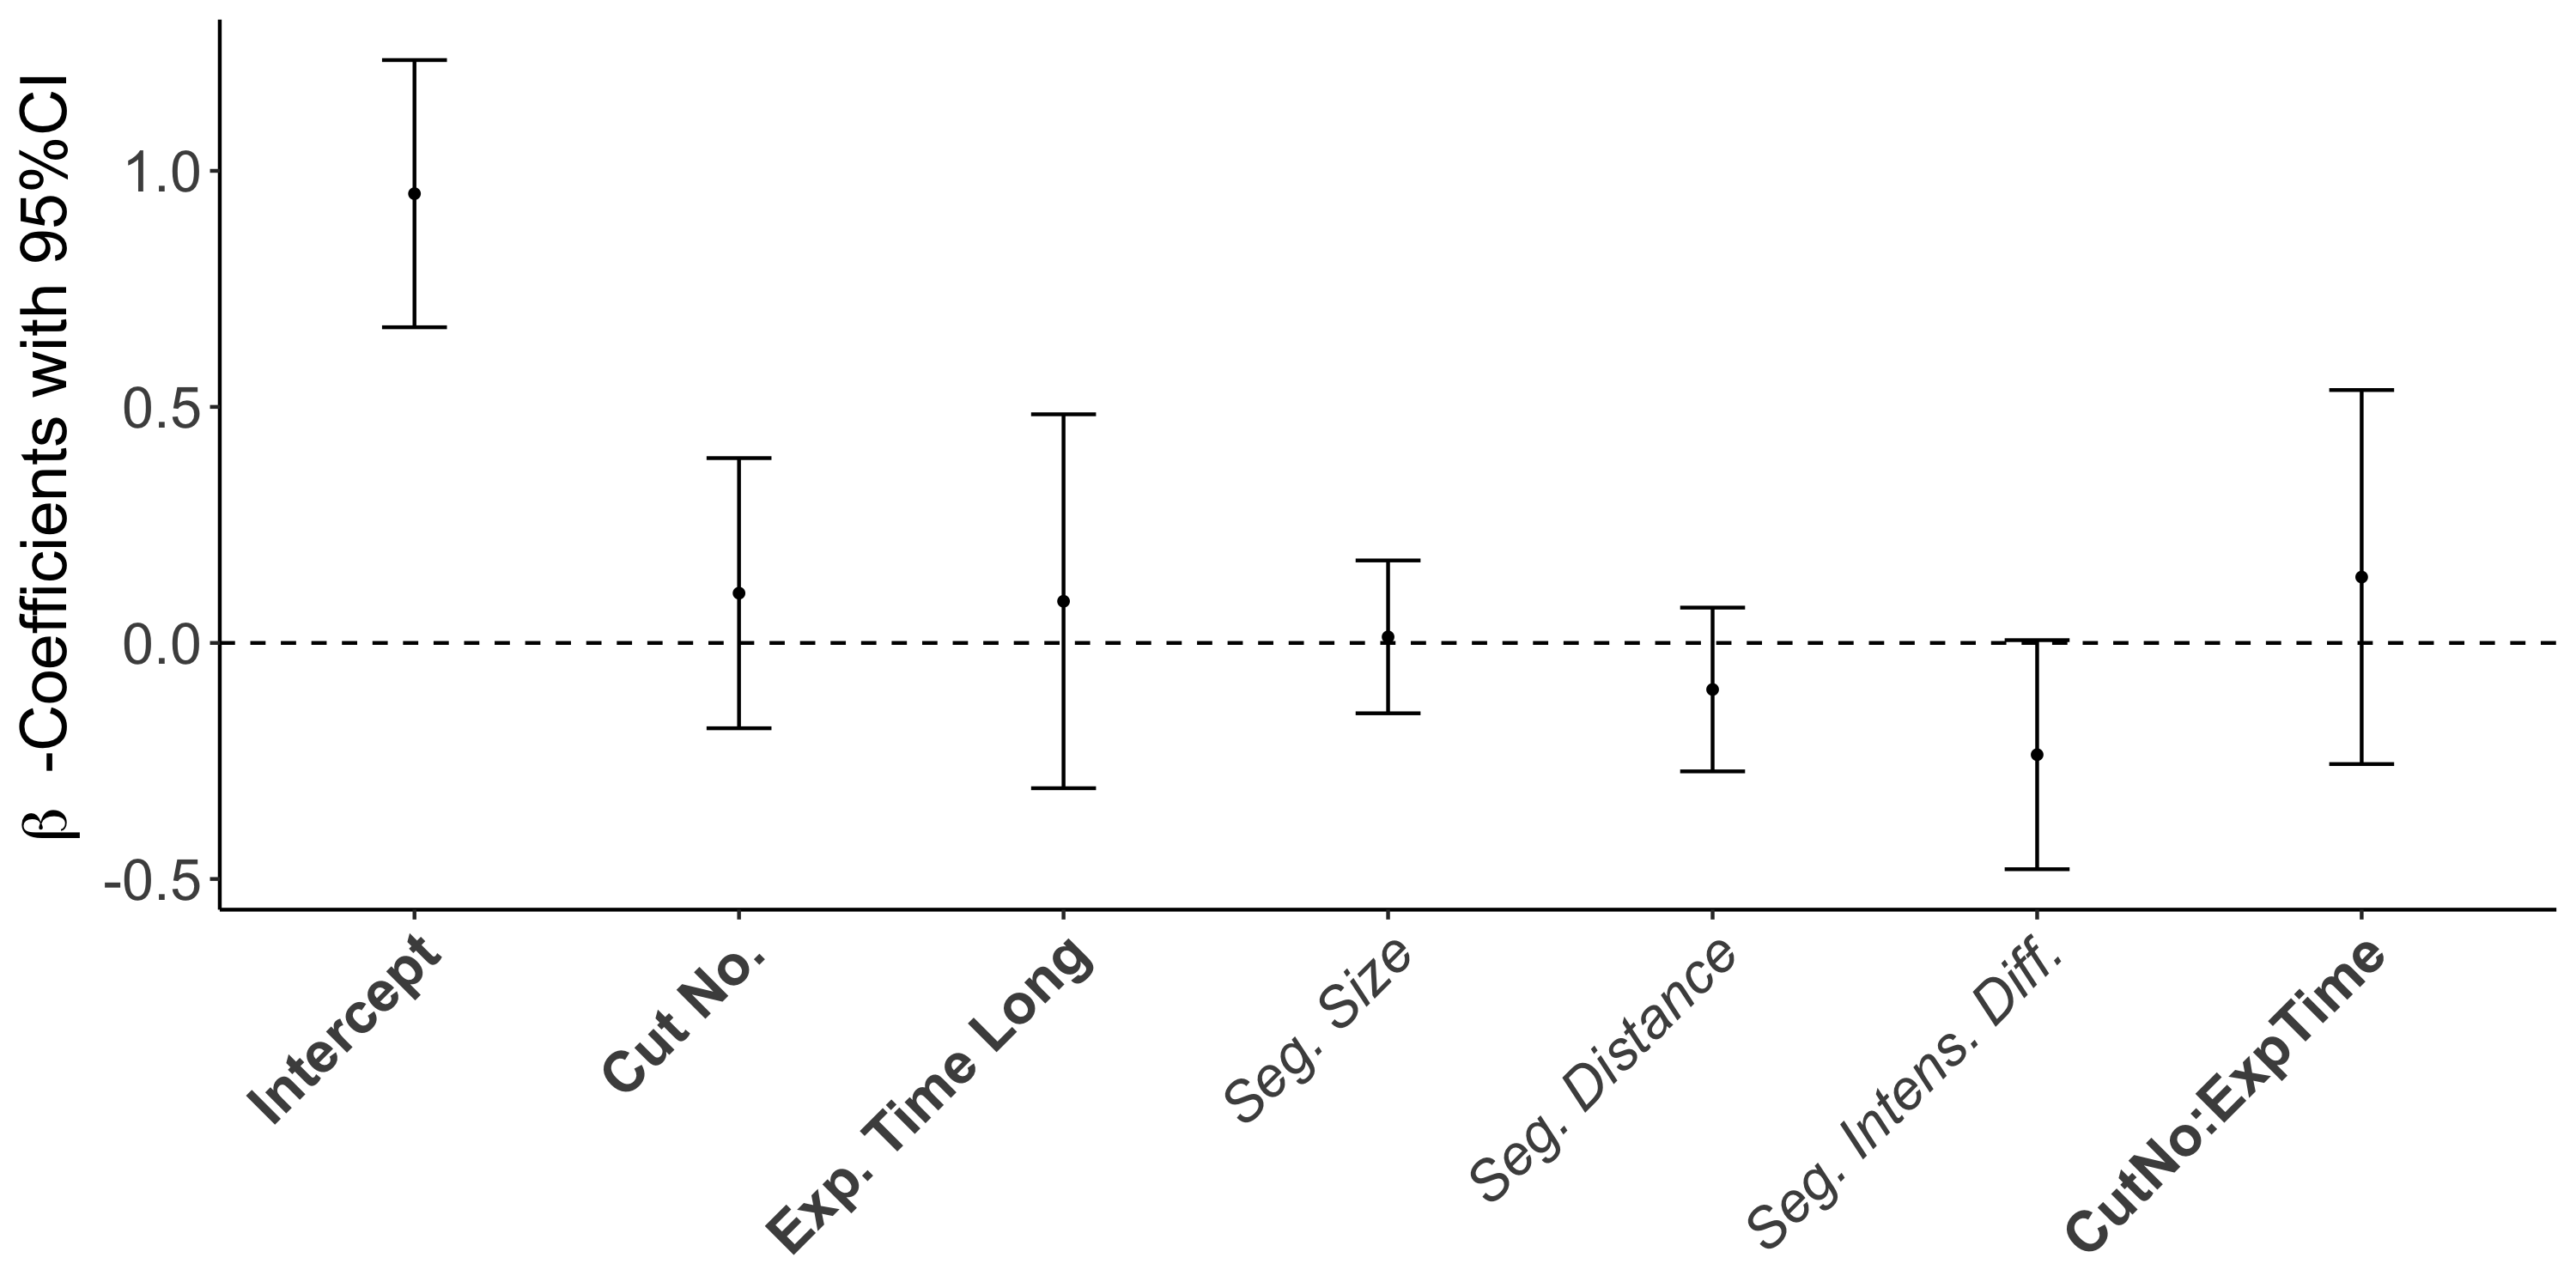
\includegraphics[width = \textwidth]{pictures/sw_cont_coefficients_othrs_tgthr.png}
        \caption{Effect of main predictors in control condition}
        \label{fig:sw_coefficients_con_main}
    \end{figure}
\end{frame}

\begin{frame}{MY - Control Results}
    \begin{figure}
        \hspace*{-1cm} 
        \centering
        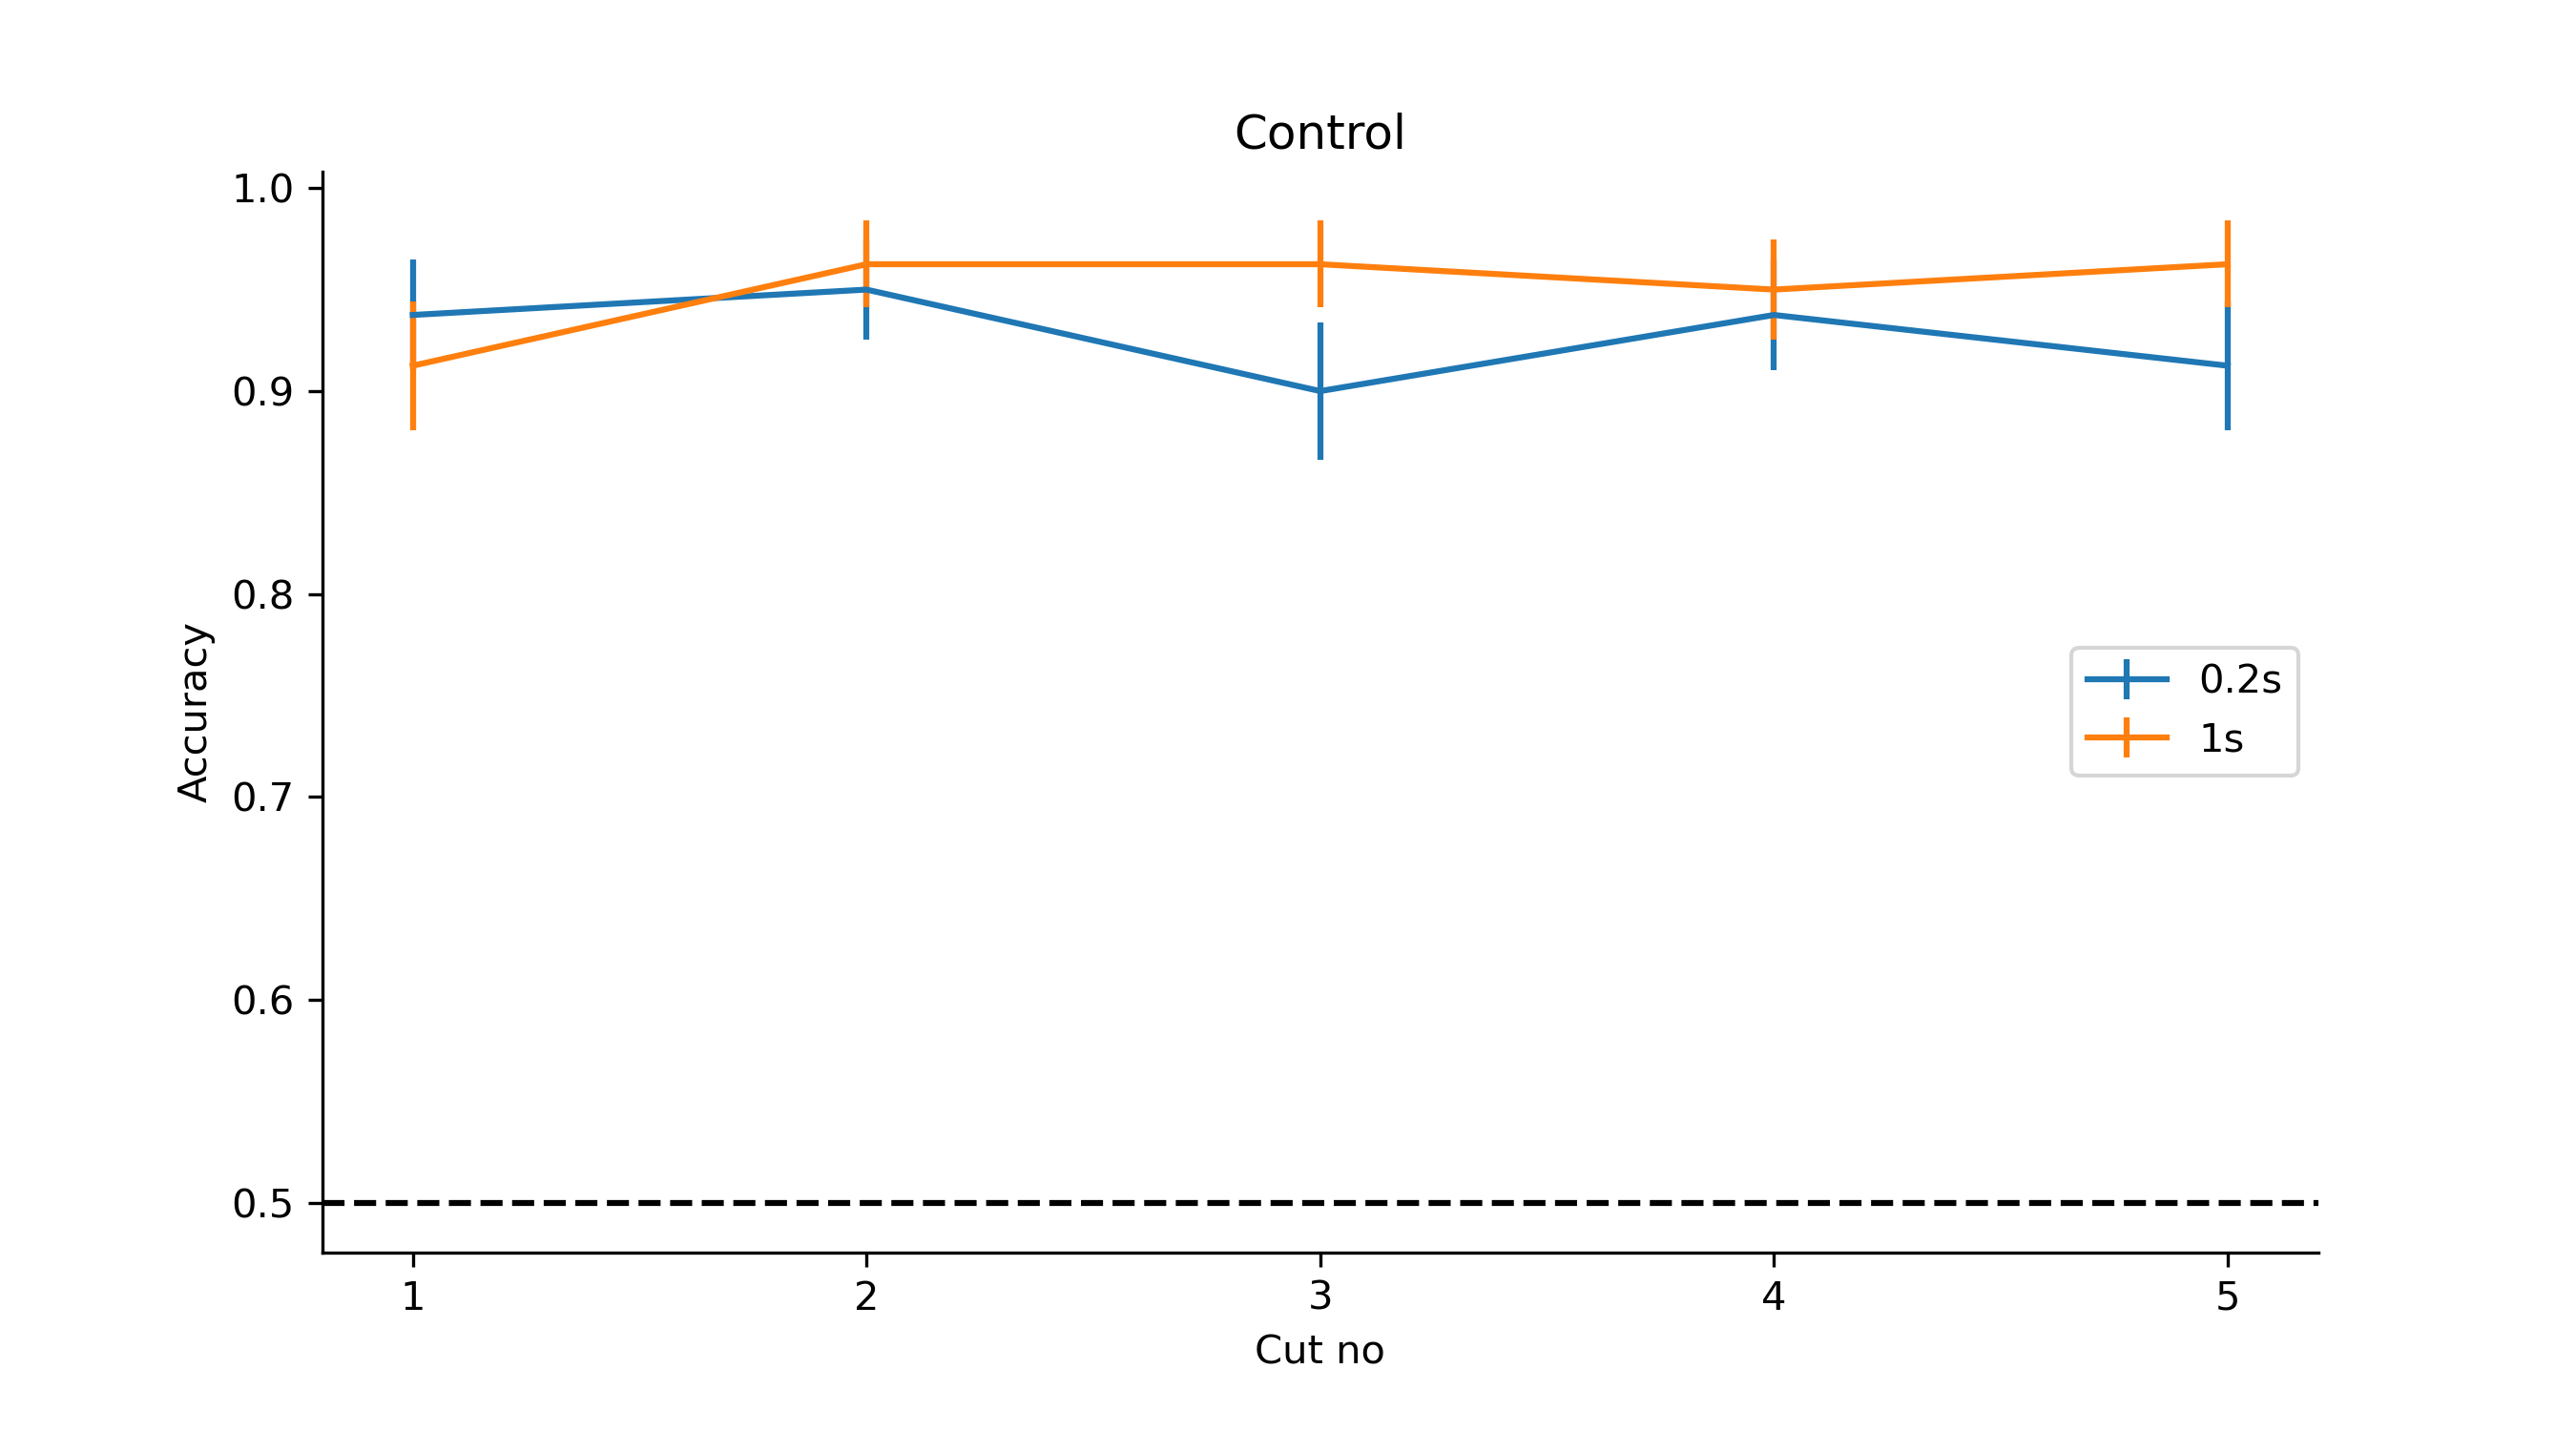
\includegraphics[width = 1.1\textwidth]{pictures/my_control.png}
        \caption{Accuracy over cut number in control trials}
        \label{fig:my_cont}
    \end{figure}    
\end{frame}



\begin{frame}{MY - Coefficients}
    \begin{figure}
        \hspace*{-1cm} 
        \centering
        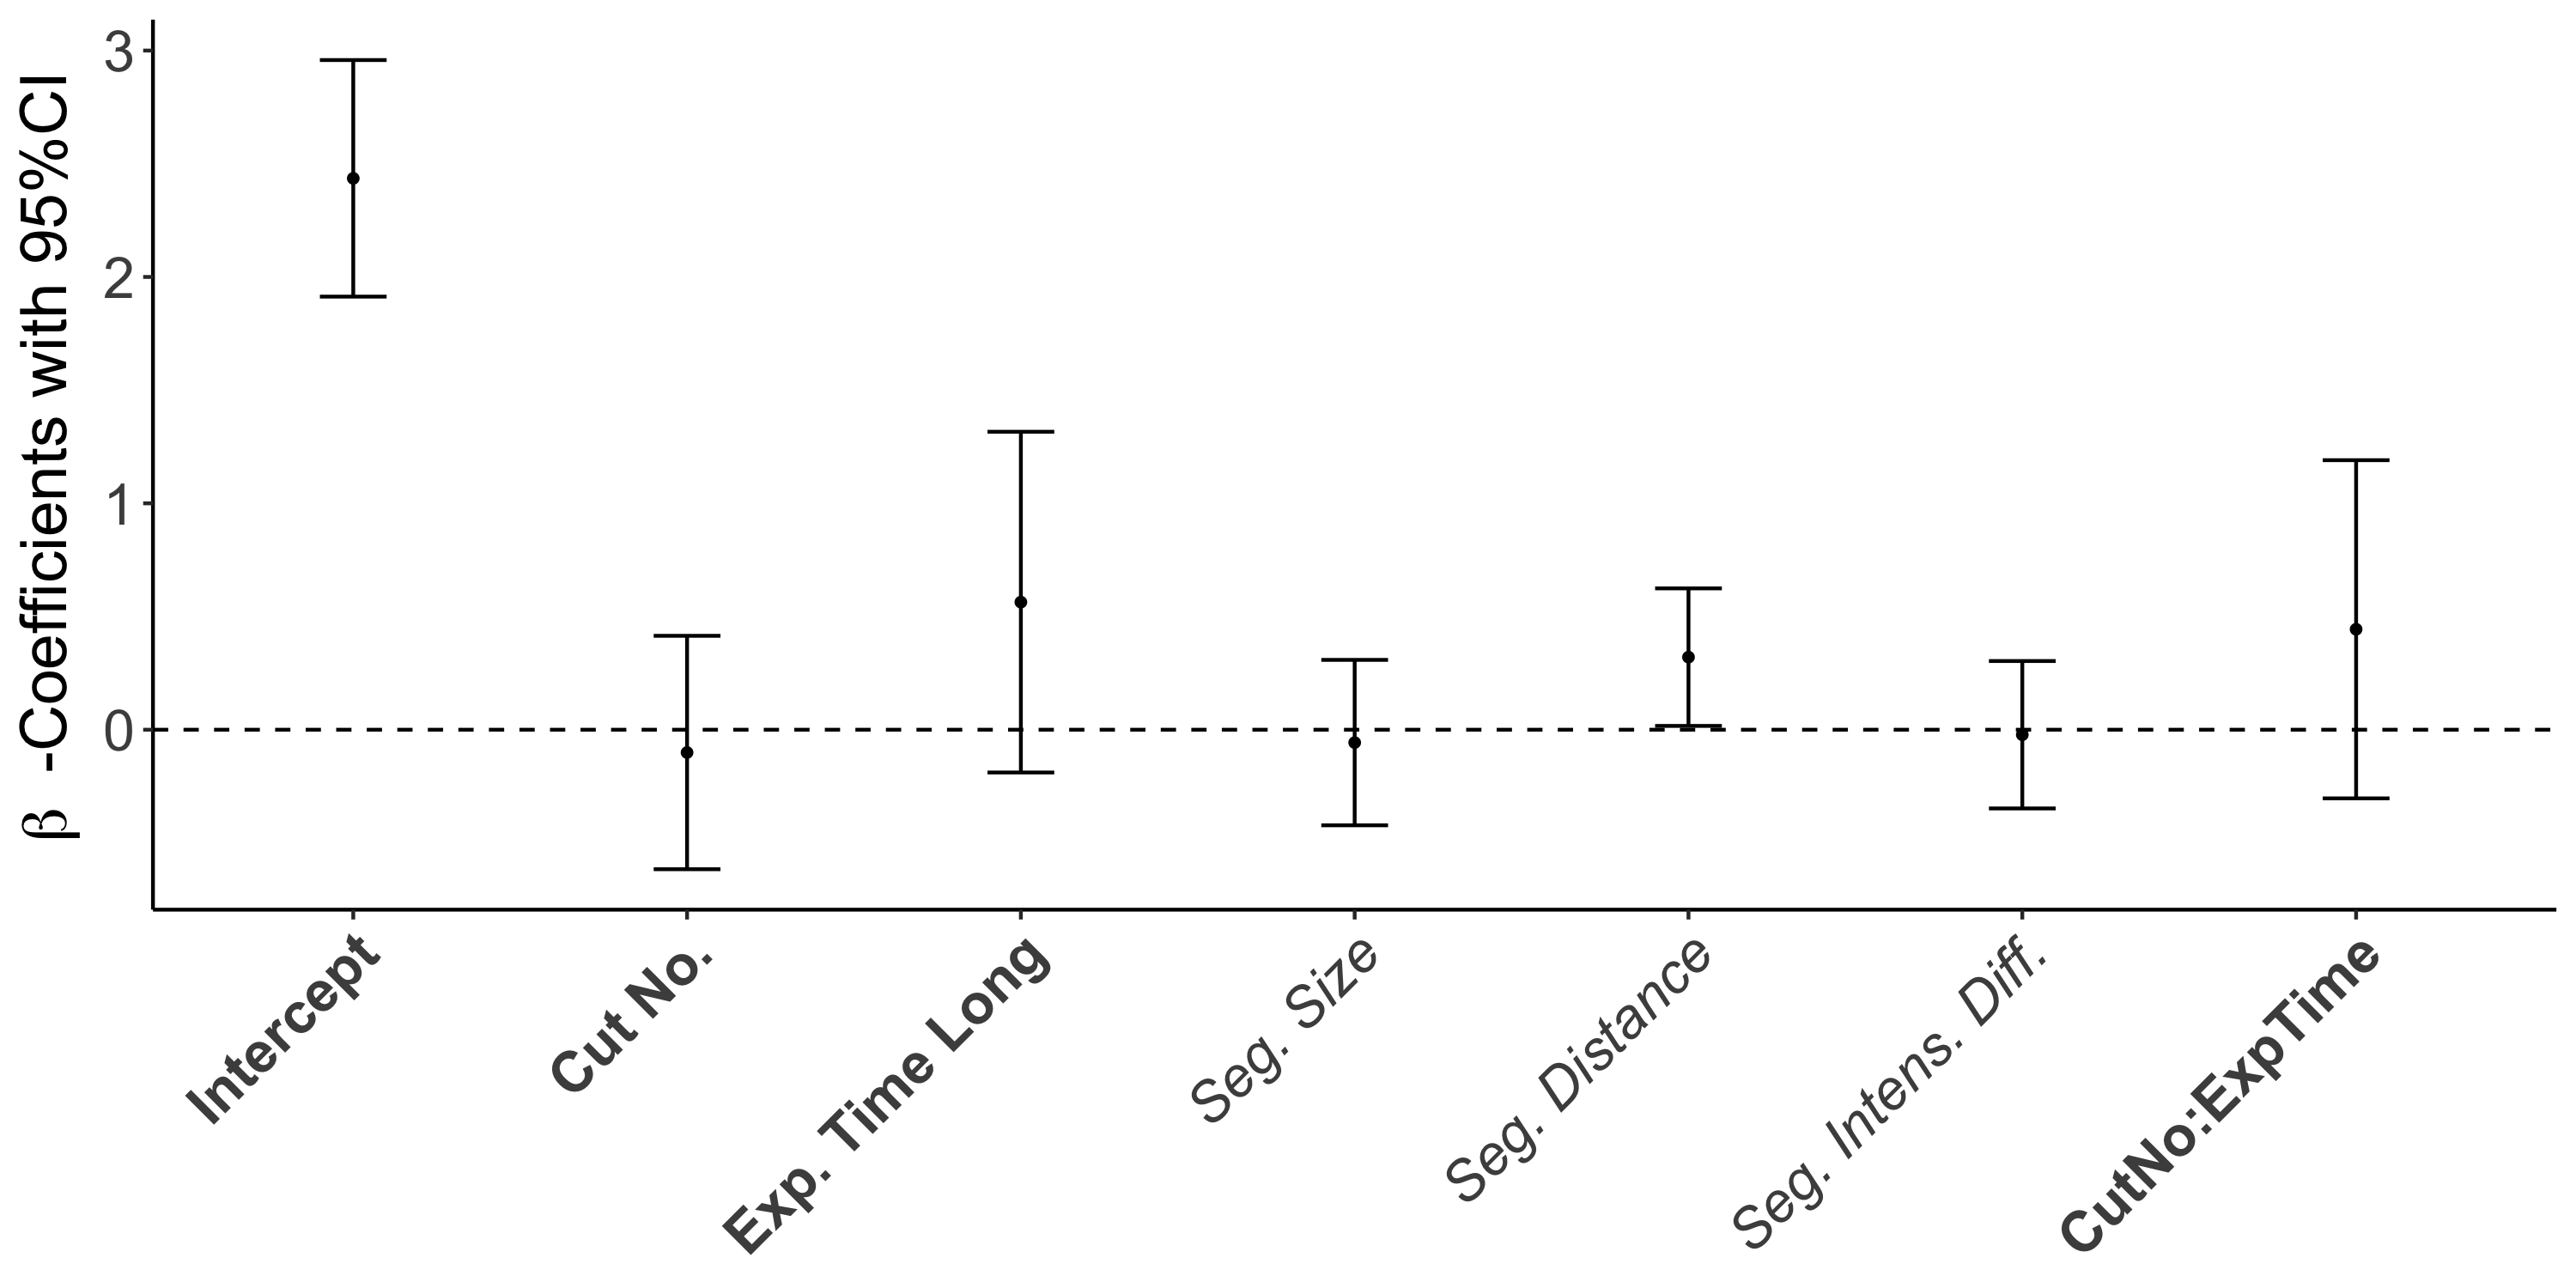
\includegraphics[width = 1.1\textwidth]{pictures/my_cont_coefficients_othrs_tgthr.png}
        \caption{Effect of alternative predictors in control condition}
        \label{fig:my_cont_coeffs_othrs}
    \end{figure}    
\end{frame}

\end{document}
